%%%%%%%%%%%%%%
%% Run LaTeX on this file several times to get Table of Contents,
%% cross-references, and citations.

%% If you have font problems, you may edit the w-bookps.sty file
%% to customize the font names to match those on your system.

%% w-bksamp.tex. Current Version: Feb 16, 2012
%%%%%%%%%%%%%%%%%%%%%%%%%%%%%%%%%%%%%%%%%%%%%%%%%%%%%%%%%%%%%%%%
%
%  Sample file for
%  Wiley Book Style, Design No.: SD 001B, 7x10
%  Wiley Book Style, Design No.: SD 004B, 6x9
%
%
%  Prepared by Amy Hendrickson, TeXnology Inc.
%  http://www.texnology.com
%%%%%%%%%%%%%%%%%%%%%%%%%%%%%%%%%%%%%%%%%%%%%%%%%%%%%%%%%%%%%%%%

%%%%%%%%%%%%%
% 7x10
%\documentclass{wileySev}

% 6x9
\documentclass{wileySix}

\usepackage{graphicx}
\usepackage{listings}
\usepackage{float}

\usepackage{color}

\definecolor{codegreen}{rgb}{0,0.6,0}
\definecolor{codegray}{rgb}{0.5,0.5,0.5}
\definecolor{codepurple}{rgb}{0.58,0,0.82}
\definecolor{backcolour}{rgb}{0.95,0.95,0.92}

\lstdefinestyle{mystyle}{
    backgroundcolor=\color{backcolour},
    commentstyle=\color{codegreen},
    keywordstyle=\color{magenta},
    numberstyle=\tiny\color{codegray},
    stringstyle=\color{codepurple},
    basicstyle=\footnotesize,
    breakatwhitespace=false,
    breaklines=true,
    captionpos=b,
    keepspaces=true,
    numbers=left,
    numbersep=5pt,
    showspaces=false,
    showstringspaces=false,
    showtabs=false,
    tabsize=2,
    language=sh
}

\lstset{style=mystyle}

%%%%%%%
%% for times math: However, this package disables bold math (!)
%% \mathbf{x} will still work, but you will not have bold math
%% in section heads or chapter titles. If you don't use math
%% in those environments, mathptmx might be a good choice.

% \usepackage{mathptmx}

% For PostScript text
\usepackage{w-bookps}

%%%%%%%%%%%%%%%%%%%%%%%%%%%%%%%%%%%%%%%%%%%%%%%%%%%%%%%%%%%%%%%%
%% Other packages you might want to use:

% for chapter bibliography made with BibTeX
% \usepackage{chapterbib}

% for multiple indices
% \usepackage{multind}

% for answers to problems
% \usepackage{answers}

%%%%%%%%%%%%%%%%%%%%%%%%%%%%%%
%% Change options here if you want:
%%
%% How many levels of section head would you like numbered?
%% 0= no section numbers, 1= section, 2= subsection, 3= subsubsection
%%==>>
\setcounter{secnumdepth}{3}

%% How many levels of section head would you like to appear in the
%% Table of Contents?
%% 0= chapter titles, 1= section titles, 2= subsection titles,
%% 3= subsubsection titles.
%%==>>
\setcounter{tocdepth}{2}

%% Cropmarks? good for final page makeup
%% \docropmarks

%%%%%%%%%%%%%%%%%%%%%%%%%%%%%%
%
% DRAFT
%
% Uncomment to get double spacing between lines, current date and time
% printed at bottom of page.
% \draft
% (If you want to keep tables from becoming double spaced also uncomment
% this):
% \renewcommand{\arraystretch}{0.6}
%%%%%%%%%%%%%%%%%%%%%%%%%%%%%%

%%%%%%% Demo of section head containing sample macro:
%% To get a macro to expand correctly in a section head, with upper and
%% lower case math, put the definition and set the box
%% before \begin{document}, so that when it appears in the
%% table of contents it will also work:

\newcommand{\VT}[1]{\ensuremath{{V_{T#1}}}}

%% use a box to expand the macro before we put it into the section head:

\newbox\sectsavebox
\setbox\sectsavebox=\hbox{\boldmath\VT{xyz}}

%%%%%%%%%%%%%%%%% End Demo


\begin{document}


\booktitle{Cerdas Menguasai Python}
\subtitle{Dalam 24 Jam}

\authors{Rolly M. Awangga\\
\affil{Informatics Research Center}
%Floyd J. Fowler, Jr.\\
%\affil{University of New Mexico}
}

\offprintinfo{Cerdas Menguasai Python, First Edition}{Rolly M. Awangga}

%% Can use \\ if title, and edition are too wide, ie,
%% \offprintinfo{Survey Methodology,\\ Second Edition}{Robert M. Groves}

%%%%%%%%%%%%%%%%%%%%%%%%%%%%%%
%%
\halftitlepage

%\titlepage


\begin{copyrightpage}{2019}
%Survey Methodology / Robert M. Groves . . . [et al.].
%\       p. cm.---(Wiley series in survey methodology)
%\    ``Wiley-Interscience."
%\    Includes bibliographical references and index.
%\    ISBN 0-471-48348-6 (pbk.)
%\    1. Surveys---Methodology.  2. Social 
%\  sciences---Research---Statistical methods.  I. Groves, Robert M.  II. %
%Series.\\
%
%HA31.2.S873 2007
%001.4'33---dc22                                             2004044064
\end{copyrightpage}

\dedication{`Jika Kamu tidak dapat menahan lelahnya belajar,
Maka kamu harus sanggup menahan perihnya Kebodohan.'
~Imam Syafi'i~}

\begin{contributors}
\name{Rolly Maulana Awangga,} Informatics Research Center., Politeknik Pos Indonesia, Bandung,
Indonesia



\end{contributors}

\contentsinbrief
\tableofcontents
\listoffigures
\listoftables
\lstlistoflistings


\begin{foreword}
Sepatah kata dari Kaprodi, Kabag Kemahasiswaan dan Mahasiswa
\end{foreword}

\begin{preface}
Buku ini diciptakan bagi yang awam dengan flask sekalipun.

\prefaceauthor{R. M. Awangga}
\where{Bandung, Jawa Barat\\
Februari, 2019}
\end{preface}


\begin{acknowledgments}
Terima kasih atas semua masukan dari para mahasiswa agar bisa membuat buku ini 
lebih baik dan lebih mudah dimengerti.

Terima kasih ini juga ditujukan khusus untuk team IRC yang 
telah fokus untuk belajar dan memahami bagaimana buku ini mendampingi proses 
Intership.
\authorinitials{R. M. A.}
\end{acknowledgments}

\begin{acronyms}
\acro{ACGIH}{American Conference of Governmental Industrial Hygienists}
\acro{AEC}{Atomic Energy Commission}
\acro{OSHA}{Occupational Health and Safety Commission}
\acro{SAMA}{Scientific Apparatus Makers Association}
\end{acronyms}

\begin{glossary}
\term{git}Merupakan manajemen sumber kode yang dibuat oleh linus torvald.

\term{bash}Merupakan bahasa sistem operasi berbasiskan *NIX.

\term{linux}Sistem operasi berbasis sumber kode terbuka yang dibuat oleh Linus Torvald
\end{glossary}

\begin{symbols}
\term{A}Amplitude

\term{\hbox{\&}}Propositional logic symbol 

\term{a}Filter Coefficient

\bigskip

\term{\mathcal{B}}Number of Beats
\end{symbols}

\begin{introduction}

%% optional, but if you want to list author:

\introauthor{Rolly Maulana Awangga, S.T., M.T.}
{Informatics Research Center\\
Bandung, Jawa Barat, Indonesia}

Pada era disruptif  \index{disruptif}\index{disruptif!modern} 
saat ini. git merupakan sebuah kebutuhan dalam sebuah organisasi pengembangan perangkat lunak.
Buku ini diharapkan bisa menjadi penghantar para programmer, analis, IT Operation dan Project Manajer.
Dalam melakukan implementasi git pada diri dan organisasinya.

Rumusnya cuman sebagai contoh aja biar keren\cite{awangga2018sampeu}.

\begin{equation}
ABC {\cal DEF} \alpha\beta\Gamma\Delta\sum^{abc}_{def}
\end{equation}

\end{introduction}

%%%%%%%%%%%%%%%%%%Isi Buku_
%TEORI
%\chapter{Judul Bagian Pertama}
%\section{Arjun Yuda Firwanda}
\subsection{Soal 1}
Isi jawaban soal ke-1

Kalau mau dibikin paragrap \textbf{cukup enter aja}, tidak usah pakai \verb|par| dsb

%\subsection{Soal 2}
%Isi jawaban soal ke-2

%\subsection{Soal 3}
%Isi jawaban soal ke-3

\section{Dwi Yulianingsih}
\subsection{Soal 1}
Isi jawaban soal ke-1

Kalau mau dibikin paragrap \textbf{cukup enter aja}, tidak usah pakai \verb|par| dsb

%\subsection{Soal 2}
%Isi jawaban soal ke-2

%\subsection{Soal 3}
%Isi jawaban soal ke-3

\section{Harun Ar-Rasyid}
\subsection{Soal 1}
Isi jawaban soal ke-1

Kalau mau dibikin paragrap \textbf{cukup enter aja}, tidak usah pakai \verb|par| dsb

%\subsection{Soal 2}
%Isi jawaban soal ke-2

%\subsection{Soal 3}
%Isi jawaban soal ke-3

\section{Sri Rahayu}
\subsection{Soal 1}
Isi jawaban soal ke-1

Kalau mau dibikin paragrap \textbf{cukup enter aja}, tidak usah pakai \verb|par| dsb

%\subsection{Soal 2}
%Isi jawaban soal ke-2

%\subsection{Soal 3}
%Isi jawaban soal ke-3

\section{Doli Jonviter}
\subsection{Soal 1}
Isi jawaban soal ke-1

Kalau mau dibikin paragrap \textbf{cukup enter aja}, tidak usah pakai \verb|par| dsb

%\subsection{Soal 2}
%Isi jawaban soal ke-2

%\subsection{Soal 3}
%Isi jawaban soal ke-3

\section{Rahmatul Ridha}
\subsection{Soal 1}
Isi jawaban soal ke-1

Kalau mau dibikin paragrap \textbf{cukup enter aja}, tidak usah pakai \verb|par| dsb

%\subsection{Soal 2}
%Isi jawaban soal ke-2

%\subsection{Soal 3}
%Isi jawaban soal ke-3

\section{Tomy Prawoto}
\subsection{Soal 1}
Isi jawaban soal ke-1

Kalau mau dibikin paragrap \textbf{cukup enter aja}, tidak usah pakai \verb|par| dsb

%\subsection{Soal 2}
%Isi jawaban soal ke-2

%\subsection{Soal 3}
%Isi jawaban soal ke-3

%PRAKTEK
%\chapter{Judul Bagian Pertama}
%\section{Arjun Yuda Firwanda}
\subsection{Soal 1}
Isi jawaban soal ke-1

Kalau mau dibikin paragrap \textbf{cukup enter aja}, tidak usah pakai \verb|par| dsb

%\subsection{Soal 2}
%Isi jawaban soal ke-2

%\subsection{Soal 3}
%Isi jawaban soal ke-3

\section{Dwi Yulianingsih}
\subsection{Soal 1}
Isi jawaban soal ke-1

Kalau mau dibikin paragrap \textbf{cukup enter aja}, tidak usah pakai \verb|par| dsb

%\subsection{Soal 2}
%Isi jawaban soal ke-2

%\subsection{Soal 3}
%Isi jawaban soal ke-3

\section{Harun Ar-Rasyid}
\subsection{Soal 1}
Isi jawaban soal ke-1

Kalau mau dibikin paragrap \textbf{cukup enter aja}, tidak usah pakai \verb|par| dsb

%\subsection{Soal 2}
%Isi jawaban soal ke-2

%\subsection{Soal 3}
%Isi jawaban soal ke-3

\section{Sri Rahayu}
\subsection{Soal 1}
Isi jawaban soal ke-1

Kalau mau dibikin paragrap \textbf{cukup enter aja}, tidak usah pakai \verb|par| dsb

%\subsection{Soal 2}
%Isi jawaban soal ke-2

%\subsection{Soal 3}
%Isi jawaban soal ke-3

\section{Doli Jonviter}
\subsection{Soal 1}
Isi jawaban soal ke-1

Kalau mau dibikin paragrap \textbf{cukup enter aja}, tidak usah pakai \verb|par| dsb

%\subsection{Soal 2}
%Isi jawaban soal ke-2

%\subsection{Soal 3}
%Isi jawaban soal ke-3

\section{Rahmatul Ridha}
\subsection{Soal 1}
Isi jawaban soal ke-1

Kalau mau dibikin paragrap \textbf{cukup enter aja}, tidak usah pakai \verb|par| dsb

%\subsection{Soal 2}
%Isi jawaban soal ke-2

%\subsection{Soal 3}
%Isi jawaban soal ke-3

\section{Tomy Prawoto}
\subsection{Soal 1}
Isi jawaban soal ke-1

Kalau mau dibikin paragrap \textbf{cukup enter aja}, tidak usah pakai \verb|par| dsb

%\subsection{Soal 2}
%Isi jawaban soal ke-2

%\subsection{Soal 3}
%Isi jawaban soal ke-3


%TEORI
%\chapter{Judul Bagian Pertama}
%\section{Arjun Yuda Firwanda}
\subsection{Soal 1}
Isi jawaban soal ke-1

Kalau mau dibikin paragrap \textbf{cukup enter aja}, tidak usah pakai \verb|par| dsb

%\subsection{Soal 2}
%Isi jawaban soal ke-2

%\subsection{Soal 3}
%Isi jawaban soal ke-3

\section{Dwi Yulianingsih}
\subsection{Soal 1}
Isi jawaban soal ke-1

Kalau mau dibikin paragrap \textbf{cukup enter aja}, tidak usah pakai \verb|par| dsb

%\subsection{Soal 2}
%Isi jawaban soal ke-2

%\subsection{Soal 3}
%Isi jawaban soal ke-3

\section{Harun Ar-Rasyid}
\subsection{Soal 1}
Isi jawaban soal ke-1

Kalau mau dibikin paragrap \textbf{cukup enter aja}, tidak usah pakai \verb|par| dsb

%\subsection{Soal 2}
%Isi jawaban soal ke-2

%\subsection{Soal 3}
%Isi jawaban soal ke-3

\section{Sri Rahayu}
\subsection{Soal 1}
Isi jawaban soal ke-1

Kalau mau dibikin paragrap \textbf{cukup enter aja}, tidak usah pakai \verb|par| dsb

%\subsection{Soal 2}
%Isi jawaban soal ke-2

%\subsection{Soal 3}
%Isi jawaban soal ke-3

\section{Doli Jonviter}
\subsection{Soal 1}
Isi jawaban soal ke-1

Kalau mau dibikin paragrap \textbf{cukup enter aja}, tidak usah pakai \verb|par| dsb

%\subsection{Soal 2}
%Isi jawaban soal ke-2

%\subsection{Soal 3}
%Isi jawaban soal ke-3

\section{Rahmatul Ridha}
\subsection{Soal 1}
Isi jawaban soal ke-1

Kalau mau dibikin paragrap \textbf{cukup enter aja}, tidak usah pakai \verb|par| dsb

%\subsection{Soal 2}
%Isi jawaban soal ke-2

%\subsection{Soal 3}
%Isi jawaban soal ke-3

\section{Tomy Prawoto}
\subsection{Soal 1}
Isi jawaban soal ke-1

Kalau mau dibikin paragrap \textbf{cukup enter aja}, tidak usah pakai \verb|par| dsb

%\subsection{Soal 2}
%Isi jawaban soal ke-2

%\subsection{Soal 3}
%Isi jawaban soal ke-3

%PRAKTEK
%\chapter{Judul Bagian Pertama}
%\section{Arjun Yuda Firwanda}
\subsection{Soal 1}
Isi jawaban soal ke-1

Kalau mau dibikin paragrap \textbf{cukup enter aja}, tidak usah pakai \verb|par| dsb

%\subsection{Soal 2}
%Isi jawaban soal ke-2

%\subsection{Soal 3}
%Isi jawaban soal ke-3

\section{Dwi Yulianingsih}
\subsection{Soal 1}
Isi jawaban soal ke-1

Kalau mau dibikin paragrap \textbf{cukup enter aja}, tidak usah pakai \verb|par| dsb

%\subsection{Soal 2}
%Isi jawaban soal ke-2

%\subsection{Soal 3}
%Isi jawaban soal ke-3

\section{Harun Ar-Rasyid}
\subsection{Soal 1}
Isi jawaban soal ke-1

Kalau mau dibikin paragrap \textbf{cukup enter aja}, tidak usah pakai \verb|par| dsb

%\subsection{Soal 2}
%Isi jawaban soal ke-2

%\subsection{Soal 3}
%Isi jawaban soal ke-3

\section{Sri Rahayu}
\subsection{Soal 1}
Isi jawaban soal ke-1

Kalau mau dibikin paragrap \textbf{cukup enter aja}, tidak usah pakai \verb|par| dsb

%\subsection{Soal 2}
%Isi jawaban soal ke-2

%\subsection{Soal 3}
%Isi jawaban soal ke-3

\section{Doli Jonviter}
\subsection{Soal 1}
Isi jawaban soal ke-1

Kalau mau dibikin paragrap \textbf{cukup enter aja}, tidak usah pakai \verb|par| dsb

%\subsection{Soal 2}
%Isi jawaban soal ke-2

%\subsection{Soal 3}
%Isi jawaban soal ke-3

\section{Rahmatul Ridha}
\subsection{Soal 1}
Isi jawaban soal ke-1

Kalau mau dibikin paragrap \textbf{cukup enter aja}, tidak usah pakai \verb|par| dsb

%\subsection{Soal 2}
%Isi jawaban soal ke-2

%\subsection{Soal 3}
%Isi jawaban soal ke-3

\section{Tomy Prawoto}
\subsection{Soal 1}
Isi jawaban soal ke-1

Kalau mau dibikin paragrap \textbf{cukup enter aja}, tidak usah pakai \verb|par| dsb

%\subsection{Soal 2}
%Isi jawaban soal ke-2

%\subsection{Soal 3}
%Isi jawaban soal ke-3


%TEORI
%\chapter{Judul Bagian Pertama}
%\section{Arjun Yuda Firwanda}
\subsection{Soal 1}
Isi jawaban soal ke-1

Kalau mau dibikin paragrap \textbf{cukup enter aja}, tidak usah pakai \verb|par| dsb

%\subsection{Soal 2}
%Isi jawaban soal ke-2

%\subsection{Soal 3}
%Isi jawaban soal ke-3

\section{Dwi Yulianingsih}
\subsection{Soal 1}
Isi jawaban soal ke-1

Kalau mau dibikin paragrap \textbf{cukup enter aja}, tidak usah pakai \verb|par| dsb

%\subsection{Soal 2}
%Isi jawaban soal ke-2

%\subsection{Soal 3}
%Isi jawaban soal ke-3

\section{Harun Ar-Rasyid}
\subsection{Soal 1}
Isi jawaban soal ke-1

Kalau mau dibikin paragrap \textbf{cukup enter aja}, tidak usah pakai \verb|par| dsb

%\subsection{Soal 2}
%Isi jawaban soal ke-2

%\subsection{Soal 3}
%Isi jawaban soal ke-3

\section{Sri Rahayu}
\subsection{Soal 1}
Isi jawaban soal ke-1

Kalau mau dibikin paragrap \textbf{cukup enter aja}, tidak usah pakai \verb|par| dsb

%\subsection{Soal 2}
%Isi jawaban soal ke-2

%\subsection{Soal 3}
%Isi jawaban soal ke-3

\section{Doli Jonviter}
\subsection{Soal 1}
Isi jawaban soal ke-1

Kalau mau dibikin paragrap \textbf{cukup enter aja}, tidak usah pakai \verb|par| dsb

%\subsection{Soal 2}
%Isi jawaban soal ke-2

%\subsection{Soal 3}
%Isi jawaban soal ke-3

\section{Rahmatul Ridha}
\subsection{Soal 1}
Isi jawaban soal ke-1

Kalau mau dibikin paragrap \textbf{cukup enter aja}, tidak usah pakai \verb|par| dsb

%\subsection{Soal 2}
%Isi jawaban soal ke-2

%\subsection{Soal 3}
%Isi jawaban soal ke-3

\section{Tomy Prawoto}
\subsection{Soal 1}
Isi jawaban soal ke-1

Kalau mau dibikin paragrap \textbf{cukup enter aja}, tidak usah pakai \verb|par| dsb

%\subsection{Soal 2}
%Isi jawaban soal ke-2

%\subsection{Soal 3}
%Isi jawaban soal ke-3

%PRAKTEK
%\chapter{Judul Bagian Pertama}
%\section{Arjun Yuda Firwanda}
\subsection{Soal 1}
Isi jawaban soal ke-1

Kalau mau dibikin paragrap \textbf{cukup enter aja}, tidak usah pakai \verb|par| dsb

%\subsection{Soal 2}
%Isi jawaban soal ke-2

%\subsection{Soal 3}
%Isi jawaban soal ke-3

\section{Dwi Yulianingsih}
\subsection{Soal 1}
Isi jawaban soal ke-1

Kalau mau dibikin paragrap \textbf{cukup enter aja}, tidak usah pakai \verb|par| dsb

%\subsection{Soal 2}
%Isi jawaban soal ke-2

%\subsection{Soal 3}
%Isi jawaban soal ke-3

\section{Harun Ar-Rasyid}
\subsection{Soal 1}
Isi jawaban soal ke-1

Kalau mau dibikin paragrap \textbf{cukup enter aja}, tidak usah pakai \verb|par| dsb

%\subsection{Soal 2}
%Isi jawaban soal ke-2

%\subsection{Soal 3}
%Isi jawaban soal ke-3

\section{Sri Rahayu}
\subsection{Soal 1}
Isi jawaban soal ke-1

Kalau mau dibikin paragrap \textbf{cukup enter aja}, tidak usah pakai \verb|par| dsb

%\subsection{Soal 2}
%Isi jawaban soal ke-2

%\subsection{Soal 3}
%Isi jawaban soal ke-3

\section{Doli Jonviter}
\subsection{Soal 1}
Isi jawaban soal ke-1

Kalau mau dibikin paragrap \textbf{cukup enter aja}, tidak usah pakai \verb|par| dsb

%\subsection{Soal 2}
%Isi jawaban soal ke-2

%\subsection{Soal 3}
%Isi jawaban soal ke-3

\section{Rahmatul Ridha}
\subsection{Soal 1}
Isi jawaban soal ke-1

Kalau mau dibikin paragrap \textbf{cukup enter aja}, tidak usah pakai \verb|par| dsb

%\subsection{Soal 2}
%Isi jawaban soal ke-2

%\subsection{Soal 3}
%Isi jawaban soal ke-3

\section{Tomy Prawoto}
\subsection{Soal 1}
Isi jawaban soal ke-1

Kalau mau dibikin paragrap \textbf{cukup enter aja}, tidak usah pakai \verb|par| dsb

%\subsection{Soal 2}
%Isi jawaban soal ke-2

%\subsection{Soal 3}
%Isi jawaban soal ke-3


%TEORI
\chapter{Library CSV dan Pandas}
%\section{Kadek Diva Krishna Murti}
\subsection{Soal 1}
\textbf{Pengenalan CSV}

Comma Separated Values (CSV) adalah suatu format data yang di mana setiap bagian data dipisahkan dengan tanda koma (,). Format CSV biasanya berfungsi untuk menukar atau mengonversi data ke format lainnya 
%\cite{shafranovich2005common}.

\textbf{Sejarah Format CSV}

IBM Fortran (level H extended) compiler di bawah OS/360 mendukung format CSV pada tahun 1972. FORTRAN 77 mendefinisakan penulisannya dimana input atau output penulisannya menggunakan tanda koma atau spasi untuk pembatas antar data dan penulisan tersebut telah disetujui pada tahun 1978.

Osborne Executive computer yang mengembangkan SuperCalc spreadsheet pada tahun 1983 membuat konvensi kutipan CSV yang memungkinkan string mengandung koma.

Inisiatif standardisasi utama - mentransformasikan "definisi fuzzy de facto" menjadi definisi yang lebih tepat dan de jure - adalah pada tahun 2005, dengan RFC4180, mendefinisikan CSV sebagai Tipe Konten MIME. Kemudian, pada 2013, beberapa kekurangan RFC4180 ditangani oleh rekomendasi W3C.

Pada 2014 IETF menerbitkan RFC7111 yang menjelaskan aplikasi fragmen URI pada dokumen CSV. RFC7111 menentukan bagaimana rentang baris, kolom, dan sel dapat dipilih dari dokumen CSV menggunakan indeks posisi.

Pada 2015 W3C, dalam upaya meningkatkan CSV dengan semantik formal, mempublikasikan draft rekomendasi pertama untuk standar metadata CSV, yang dimulai sebagai rekomendasi pada bulan Desember tahun yang sama.

\textbf{Contoh penggunaan format CSV}

\lstinputlisting[caption = Contoh penggunaan format CSV., firstline=1, lastline=3]{src/4/1174006/Teori/teori.csv}

\subsection{Soal 2}
Aplikasi-aplikasi yang dapat menciptkan file csv, yaitu:

\begin{enumerate}
	\item Editor teks (Notepad, Sublime, Atom, dan lain-lain)
	\item Spreadsheet (Microsoft Excel dan lain-lain)
\end{enumerate}

\subsection{Soal 3}
Cara menulis dan membaca file csv di excel atau spreadsheet, sebagai berikut:

\textbf{Menulis File CSV}

\begin{enumerate}
	\item Pertama silahkan buka aplikasi Excel dengan cara klik ''Start'', cari Excel, kemudian tekan Enter.
	
	\begin{figure}[H]
		\includegraphics[width=9cm]{figures/4/1174006/Teori/t1.png}
		\centering
	\end{figure}
	
	\item Setelah aplikasi terbuka silahkan klik ''Blank Workbook''.
	
	\begin{figure}[H]
		\includegraphics[width=10cm]{figures/4/1174006/Teori/t2.png}
		\centering
	\end{figure}
	
	\item Kemudian isi sesuai dengan data yang ingin dibuat.
	
	\begin{figure}[H]
		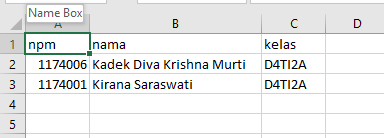
\includegraphics[width=10cm]{figures/4/1174006/Teori/t3.png}
		\centering
	\end{figure}
	
	\item Setelah selesai dibuat, silahkan simpan file tersebut dengan cara mengklik ''File'', lalu klik ''Save''.
	
	\begin{figure}[H]
		\includegraphics[width=10cm]{figures/4/1174006/Teori/t4.png}
		\centering
	\end{figure}
	
	\item Kemudian isi kolom ''File name'' dengan nama file anda dan kolom ''Save as type'' pilih yang berekstensi .csv.
	
	\begin{figure}[H]
		\includegraphics[width=9cm]{figures/4/1174006/Teori/t5.png}
		\centering
	\end{figure}
	
	\item Lalu tinggal klik ''Yes''.
	
	\begin{figure}[H]
		\includegraphics[width=7cm]{figures/4/1174006/Teori/t6.png}
		\centering
	\end{figure}
	
	\item Kemudian file yang Anda telah terbuat tadi tersimpan dengan ekstensi .csv. Untuk melihat isi filenya tinggal klik dua kali pada file tersebut.
	
	\begin{figure}[H]
		
\includegraphics[width=10cm]{figures/4/1174006/Teori/t8.png}
		\centering
	\end{figure}
	
	\item Berikut ini adalah isi dari file yang tadi Anda buat.
	
	\begin{figure}[H]
		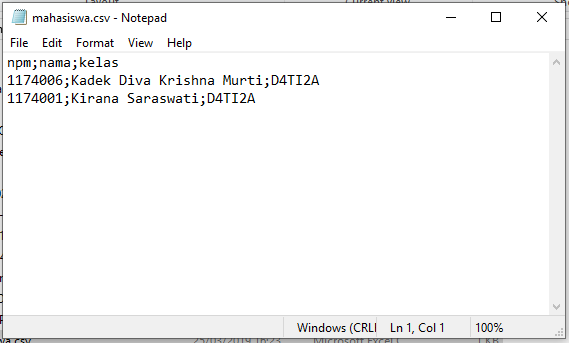
\includegraphics[width=8cm]{figures/4/1174006/Teori/t7.png}
		\centering
	\end{figure}
\end{enumerate}

\textbf{Melihat File CSV di Excel atau Spreadsheet}

\begin{enumerate}
	\item Pertama klik dua kali pada file yang yang berekstensi CSV.
	
	\begin{figure}[H]
		
\includegraphics[width=10cm]{figures/4/1174006/Teori/t8.png}
		\centering
	\end{figure}
	
	\item Kemudian file akan terbuka secara otomatis di aplikasi Excel atau spreadsheet.
	
	\begin{figure}[H]
		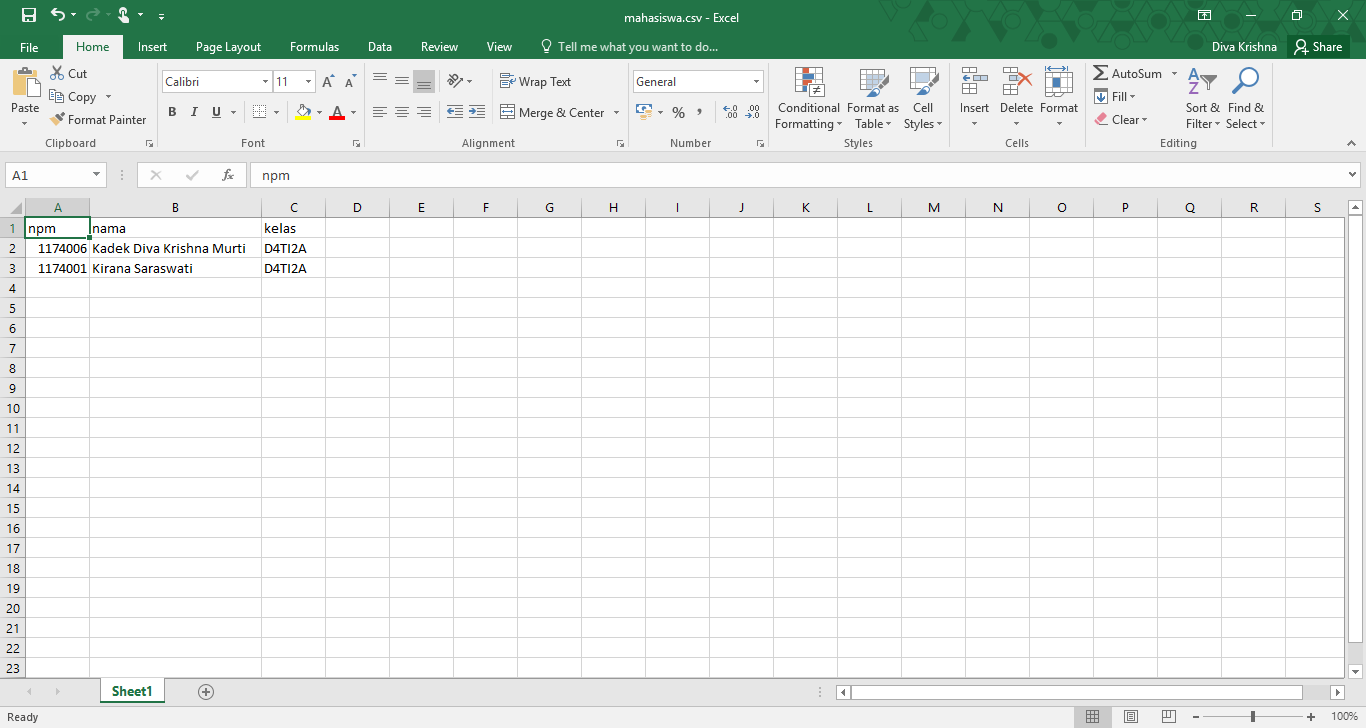
\includegraphics[width=10cm]{figures/4/1174006/Teori/t9.png}
		\centering
	\end{figure}
\end{enumerate}

\subsection{Soal 4}
Sejarah library csv

Library csv mengimplementasikan kelas untuk membaca dan menulis data tabular dalam format CSV. Hal ini memungkinkan programmer untuk mengatakan, "tulis data ini dalam format yang disukai oleh Excel," atau "baca data dari file ini yang dihasilkan oleh Excel," tanpa mengetahui detail yang tepat dari format CSV yang digunakan oleh Excel. Pemrogram juga dapat menggambarkan format CSV yang dipahami oleh aplikasi lain atau menentukan format CSV tujuan khusus mereka sendiri.

\subsection{Soal 5}
Sejarah library pandas

Pada 2008, pengembangan pandas dimulai di AQR Capital Management. Pada akhir 2009 telah menjadi open source, dan secara aktif didukung hari ini oleh komunitas individu yang berpikiran sama di seluruh dunia yang menyumbangkan waktu dan energi berharga mereka untuk membantu membuat panda open source menjadi mungkin.

Sejak 2015, pandas adalah proyek yang disponsori NumFOCUS. Ini akan membantu memastikan keberhasilan pengembangan panda sebagai proyek sumber terbuka kelas dunia.

\subsection{Soal 6}
Fungsi-fungsi yang terdapat di library csv, yaitu:
\begin{enumerate}
	\item reader
	
	Fungsi ini digunakan untuk membaca isi file berformat CSV dari list.
	
	\lstinputlisting[caption = Membaca file berformat CSV list., firstline=7, lastline=13]{src/4/1174006/Teori/1174006.py}
	
	\item DictReader
	
	Fungsi ini digunakan untuk membaca isi file berformat CSV dari dictionary.
	
	\lstinputlisting[caption =  Membaca file berformat CSV dictionary., firstline=15, lastline=21]{src/4/1174006/Teori/1174006.py}
	
	\item write
	
	Fungsi ini digunakan untuk menulis file berformat CSV dari list.
	
	\lstinputlisting[caption =  Menulis file berformat CSV list., firstline=23, lastline=30]{src/4/1174006/Teori/1174006.py}
	
	\item DictWrite
	
	Fungsi ini digunakan untuk menulis file berformat CSV dari dictionary.
	
	\lstinputlisting[caption =  Menulis file berformat CSV dictionary., firstline=32, lastline=41]{src/4/1174006/Teori/1174006.py}
	
\end{enumerate}

\subsection{Soal 7}
Fungsi-fungsi yang terdapat di library pandas, yaitu:
\begin{enumerate}
	\item read\_csv
	
	Fungsi ini digunakan untuk membaca isi file berformat CSV
	
	\lstinputlisting[caption =  Membaca file berformat CSV pandas., firstline=43, lastline=47]{src/4/1174006/Teori/1174006.py}
	
	\item to\_csv
	
	Fungsi ini digunakan untuk menulis file berformat CSV
	
	\lstinputlisting[caption =  Menulis file berformat CSV pandas., firstline=49, lastline=53]{src/4/1174006/Teori/1174006.py}
	
\end{enumerate}

\subsection{Kode Program Teori}
\begin{figure}[H]
	\includegraphics[width=10cm]{figures/4/1174006/Teori/kode_teori1.png}
	\centering
\end{figure}

\begin{figure}[H]
	\includegraphics[width=10cm]{figures/4/1174006/Teori/kode_teori2.png}
	\centering
\end{figure}

\subsection{Cek Plagiat Teori}

\begin{figure}[H]
	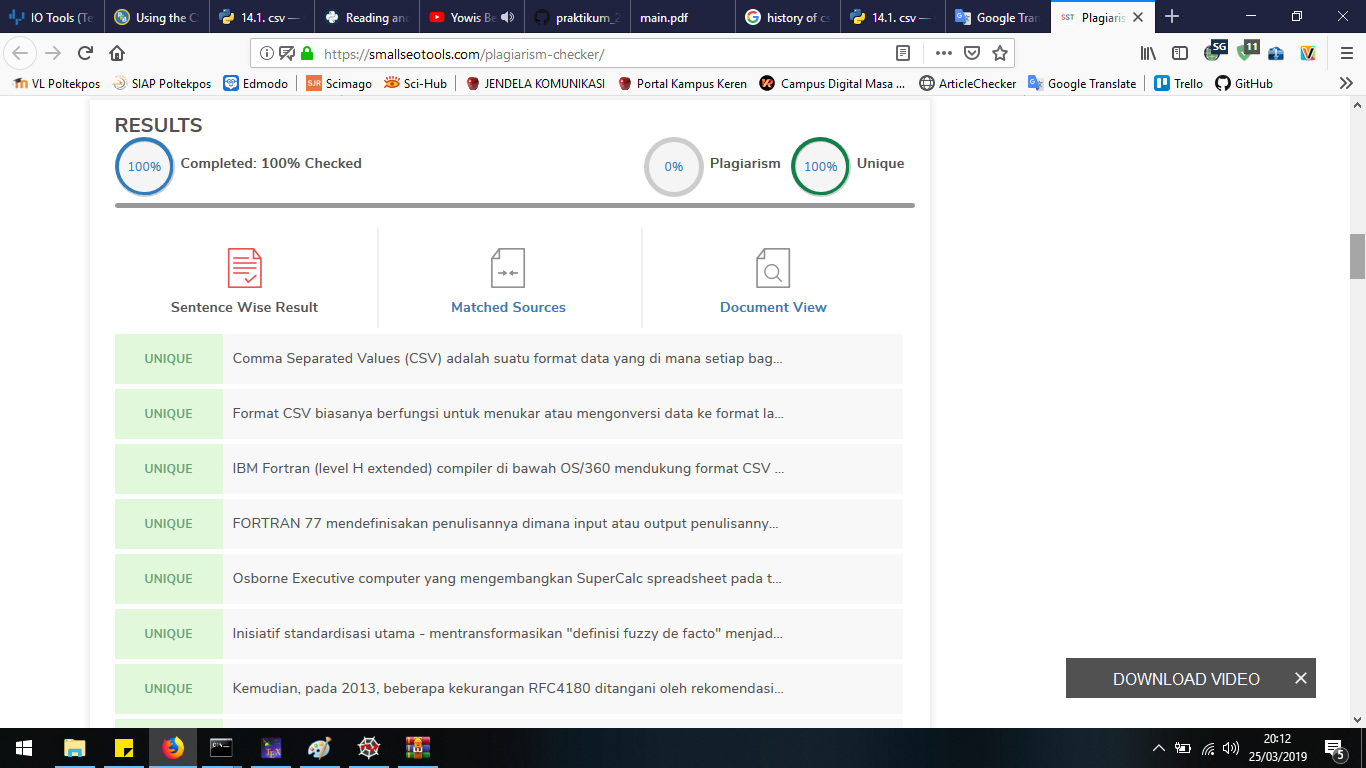
\includegraphics[width=10cm]{figures/4/1174006/Teori/plagiat_teori.png}
	\centering
\end{figure}


\section{Damara Benedikta}
\subsection{Soal 1}
 CSV (Comma Separated Value) merupakan suatu  format basis data sederhana yang dimana setiap record yang ada dipisahkan dengan tanda koma (,) atau titik koma (;). Format data file csv dapat diolah dengan berbagai text editor dengan mudah. Anda tidak perlu (dan Anda tidak akan) membuat pengurai CSV Anda sendiri dari awal. Ada beberapa perpustakaan yang dapat diterima yang dapat Anda gunakan. Pustaka csv Python akan berfungsi untuk sebagian besar kasus. Jika pekerjaan Anda memerlukan banyak data atau analisis numerik, panda library juga memiliki kemampuan penguraian CSV, yang seharusnya menangani sisanya. Dalam bahasa pemrograman Python telah disediakan modul csv yang khusus untuk mengolah data berformat csv.  Untuk memanipulasi data csv dengan python tentunya yang pertama dilakukan adalah mengimport modul csv dengan perintah import csv. File CSV biasanya dibuat oleh program yang menangani sejumlah besar data. Mereka adalah cara yang nyaman untuk mengekspor data dari spreadsheet dan basis data serta mengimpor atau menggunakannya dalam program lain. Misalnya, Anda dapat mengekspor hasil program penambangan data ke file CSV dan kemudian mengimpornya ke dalam spreadsheet untuk menganalisis data, menghasilkan grafik untuk presentasi, atau menyiapkan laporan untuk publikasi. Contoh nya adalah sebagai berikut :

 \lstinputlisting[firstline=8, lastline=20]{src/4/1174012/Teori/damdam.py}

\subsection{Soal 2} 
 Ada beberapa aplikasi yang dapat menciptakan file dengan format csv diantaranya google sheet, number di MacOS dan microsoft excel.

\subsection{Soal 3}
 Cara membuat file csv di excel cukup mudah yaitu :
\begin{itemize}
	\item Buat foldernya
	\item Pilih save as
	\item pilih file dengan format csv
\end{itemize}
Cara membaca file di csv :
\begin{itemize}
	\item Klik data - get external data - form text
	\item Akan muncul Text Import Wizard, arahkan pada file csv yang ingin anda buka lalu Open.
	\item Setelah File terbuka, akan muncul Text Import Wizard.
	\item Pilih Delimited, Kemudian Next (Di sini, bisa juga menentukan baris awal yang akan di import)
	\item Centrang pada Tab dan Comma (Atau sesuai pengaturan File Anda) lalu Next.
	\item Atur Format data pada tiap kolom yang tampil dan klik Finish
\end{itemize}

\subsection{Soal 4}
 CSV digunakan untuk memudahkan data science dan analis karena dinilai terdapat banyak kemudahan yang diperoleh. CSV dapat dimaksimalkan jika dipaduka dengan python karena python adalah bahasa pemrograman yang support ke banyak library termasuk csv. Maka karena itulah perpaduan python dan csv seringkali digunakan oleh perusahaan-perushaan besar dalam mengolah datanya.

\subsection{Soal 5}
Pandas merupakan sebuah tool yang dapat digunakan sebagai alat analisis data dan struktur untuk bahasa pemrograman Python. Pandas dapat mengolah data dengan mudah, salah satu fitur yang ada dalam pandas adalah Dataframe. Fitur dataframe dapat membaca sebuah file dan menjadikannya tabble, juga dapat mengolah suatu data dengan menggunakan operasi seperti join, group by dan teknik lainnya yang terdapat pada SQL. Dalam hal ini pandas tidak jauh beda dengan csv yaitu memiliki keunggulan dalam pengolahan data-data besar dan dapat disupport dengan baik dengan python walaupun mengimport data dalam jumlah banyak.

\subsection{Soal 6}
 Library csv memiliki keunggula-keunggulan dibandingkan format data lainnya merupakah soal kompatibilitas. File csv dapat digunakan, diolah, diekspor/impor, dan dimodifikasi menggunakan berbagai macam perangkat lunak dan bahasa pemrograman. Pada library csv mempunyai fungsi import dan eksport data yang baik dan bisa digunakan dalam jumlah besar.

\subsection{Soal 7}
pandas menyediakan beberapa fungsi operasi untuk mengolah data. Contoh jika menggunakan series bisa mencari nilai max, min, dan mean secara langsung, bahkan juga bisa melakukan operasi perpangkatan pada nilai Series secara langsung.
Pandas dapat mengolah suatu data dan mengolahnya seperti join, distinct, group by, agregasi, dan teknik seperti pada SQL. Hanya saja dilakukan pada tabel yang dimuat dari file ke RAM.


\subsection{bukti bebas plagiarisme}
\begin{figure}[H]
\centering
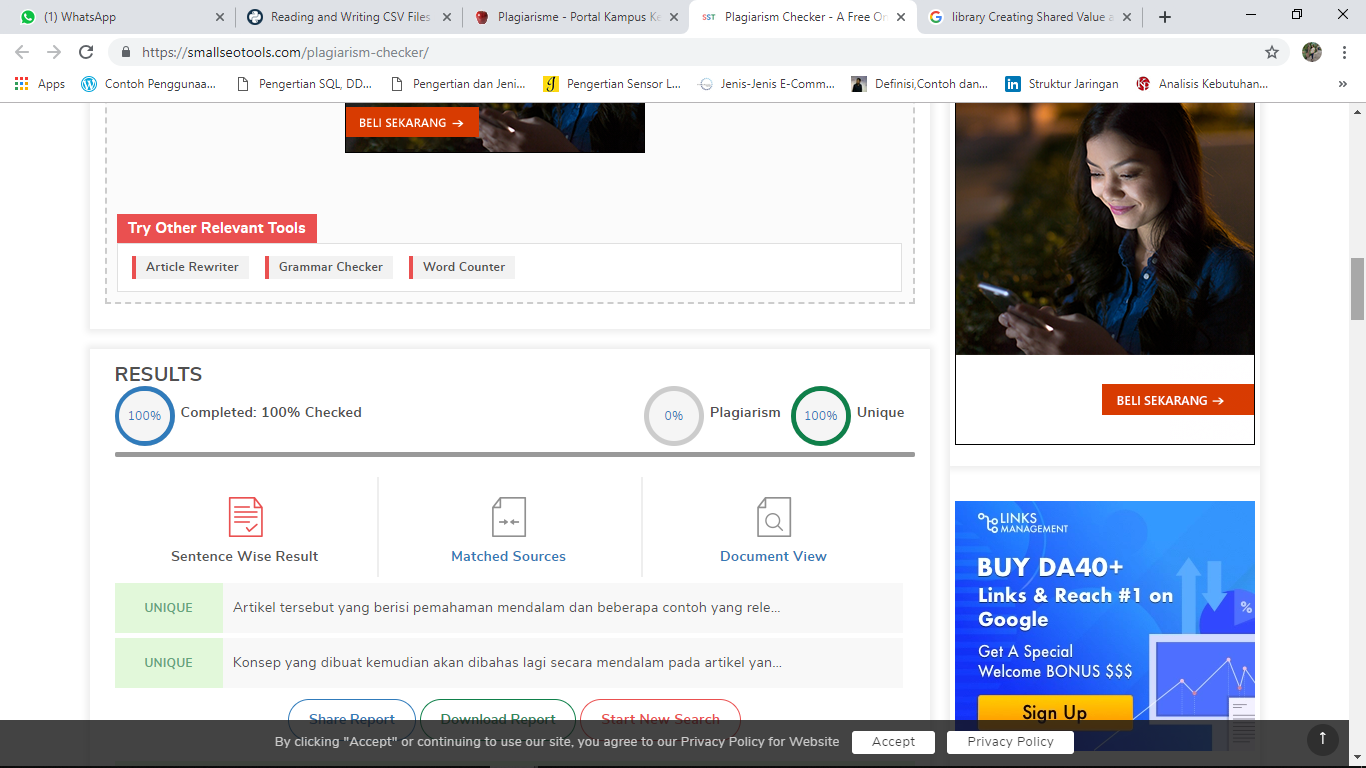
\includegraphics[width=10cm]{figures/4/1174012/Teori/ss1.png}
\caption{SS Bebas Plagiarisme}
\label{damara}
\end{figure}
%%%%%%%%%%%%%%%%%%%%%%%%%%%%%%%%%%%%%%%%%%%%%%
\section{Felix Setiawan Lase}
\subsection{Soal 1}
\textbf{Pengenalan CSV}

File CSV (Nilai Terbatas Koma) adalah jenis file khusus yang dapat Anda buat atau edit di Excel. File CSV menyimpan informasi yang disimpan dengan koma alih-alih menyimpan informasi dalam kolom.

\textbf{Sejarah Format CSV}

Kompiler Fortran IBM (tingkat lanjut H) di bawah OS / 360 mendukung format CSV pada tahun 1972. FORTRAN 77 mendefinisikan penulisannya di mana penulisan input atau output menggunakan koma atau spasi untuk batas antara data dan penulisan disetujui pada tahun 1978.

Pada 2014 IETF menerbitkan RFC7111 yang menjelaskan penerapan fragmen URI dalam dokumen CSV. RFC7111 menentukan bagaimana berbagai baris, kolom, dan sel dapat dipilih dari dokumen CSV menggunakan indeks posisi.

Pada 2015, W3C, dalam upaya meningkatkan CSV dengan semantik formal, menerbitkan rancangan rekomendasi pertama untuk standar metadata CSV, yang dimulai sebagai rekomendasi pada bulan Desember tahun yang sama.

\textbf{Contoh penggunaan format CSV}

\lstinputlisting[caption = Contoh penggunaan format CSV., firstline=1, lastline=3]{src/4/1174026/Teori/teori.csv}

\subsection{Soal 2}
Aplikasi-aplikasi yang dapat menciptkan file csv, yaitu:

\begin{enumerate}
	\item Editor teks (Notepad, Sublime, Atom, dan lain-lain)
	\item Spreadsheet (Microsoft Excel dan lain-lain)
\end{enumerate}

\subsection{Soal 3}
Cara menulis dan membaca file csv di excel atau spreadsheet, sebagai berikut:

\textbf{Menulis File CSV}

\begin{enumerate}
	\item Pertama silahkan buka aplikasi Excel dengan cara klik ''Start'', cari Excel, kemudian tekan Enter.
	
	\begin{figure}[H]
		\includegraphics[width=9cm]{figures/4/1174026/Teori/t1.png}
		\centering
	\end{figure}
	
	\item Setelah aplikasi terbuka silahkan klik ''Blank Workbook''.
	
	\begin{figure}[H]
		\includegraphics[width=10cm]{figures/4/1174026/Teori/t2.png}
		\centering
	\end{figure}
	
	\item Kemudian isi sesuai dengan data yang ingin dibuat.
	
	\begin{figure}[H]
		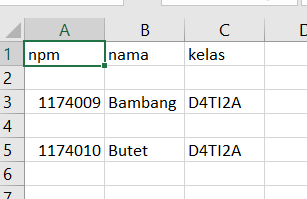
\includegraphics[width=10cm]{figures/4/1174026/Teori/t3.png}
		\centering
	\end{figure}
	
	\item Setelah selesai dibuat, silahkan simpan file tersebut dengan cara mengklik ''File'', lalu klik ''Save''.
	
	\begin{figure}[H]
		\includegraphics[width=10cm]{figures/4/1174026/Teori/t4.png}
		\centering
	\end{figure}
	
	\item Kemudian isi kolom ''File name'' dengan nama file anda dan kolom ''Save as type'' pilih yang berekstensi .csv.
	
	\begin{figure}[H]
		\includegraphics[width=9cm]{figures/4/1174026/Teori/t5.png}
		\centering
	\end{figure}
	
	\item Lalu tinggal klik ''Yes''.
	
	\begin{figure}[H]
		\includegraphics[width=7cm]{figures/4/1174026/Teori/t6.png}
		\centering
	\end{figure}
	
	\item Kemudian file yang Anda telah terbuat tadi tersimpan dengan ekstensi .csv. Untuk melihat isi filenya tinggal klik dua kali pada file tersebut.
	
	\begin{figure}[H]
		
\includegraphics[width=10cm]{figures/4/1174026/Teori/t8.png}
		\centering
	\end{figure}
	
	\item Berikut ini adalah isi dari file yang tadi Anda buat.
	
	\begin{figure}[H]
		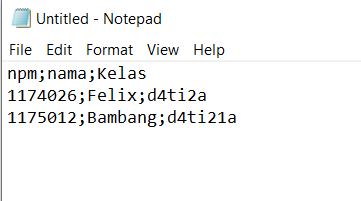
\includegraphics[width=8cm]{figures/4/1174026/Teori/t7.png}
		\centering
	\end{figure}
\end{enumerate}

\textbf{Melihat File CSV di Excel atau Spreadsheet}

\begin{enumerate}
	\item Pertama klik dua kali pada file yang yang berekstensi CSV.
	
	\begin{figure}[H]
		
\includegraphics[width=10cm]{figures/4/1174026/Teori/t8.png}
		\centering
	\end{figure}
	
	\item Kemudian file akan terbuka secara otomatis di aplikasi Excel atau spreadsheet.
	
	\begin{figure}[H]
		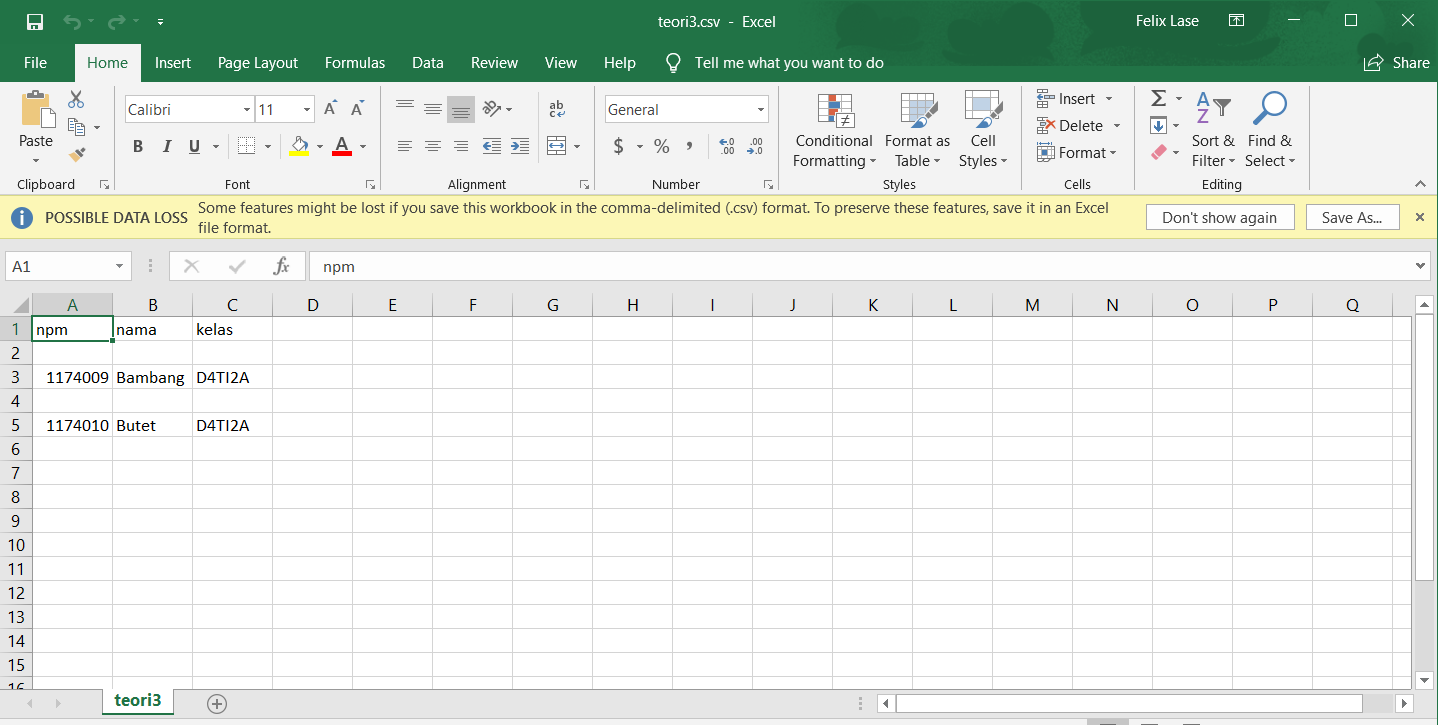
\includegraphics[width=10cm]{figures/4/1174026/Teori/t9.png}
		\centering
	\end{figure}
\end{enumerate}

\subsection{Soal 4}
Sejarah library csv

Perpustakaan CSV mengimplementasikan kelas untuk membaca dan menulis data tabular dalam format CSV. Ini memungkinkan programmer untuk mengatakan, "tulis data ini dalam format yang disukai Excel," atau "baca data dari file ini yang dihasilkan oleh Excel," tanpa mengetahui detail pasti dari format CSV yang digunakan oleh Excel. Pemrogram juga dapat menggambarkan format CSV yang dimengerti oleh aplikasi lain atau menentukan format CSV spesifik mereka sendiri.
	

\subsection{Soal 5}
Sejarah library pandas

Tahun 2008, pengembangan profesional dimulai di AQR Capital Management. Pada akhir 2009 ini telah menjadi open source, dan secara aktif didukung hari ini oleh komunitas individu yang berpikiran sama di seluruh dunia yang menyumbangkan waktu dan energi berharga mereka untuk membantu membuat panda open source menjadi mungkin.

	Sejak tahun 2015, Pandas adalah proyek yang disponsori oleh NumFOCUS. Ini akan membantu memastikan keberhasilan pengembangan Panda sebagai proyek open source kelas dunia.
	

\subsection{Soal 6}
Fungsi-fungsi yang terdapat di library csv, yaitu:
\begin{enumerate}
	\item reader
	
	Fungsi ini digunakan untuk membaca isi file berformat CSV dari list.
	
	\lstinputlisting[caption = Membaca file berformat CSV list., firstline=7, lastline=13]{src/4/1174026/Teori/1174026.py}
	
	\item DictReader
	
	Fungsi ini digunakan untuk membaca isi file berformat CSV dari dictionary.
	
	\lstinputlisting[caption =  Membaca file berformat CSV dictionary., firstline=15, lastline=21]{src/4/1174026/Teori/1174026.py}
	
	\item write
	
	Fungsi ini digunakan untuk menulis file berformat CSV dari list.
	
	\lstinputlisting[caption =  Menulis file berformat CSV list., firstline=23, lastline=30]{src/4/1174026/Teori/1174026.py}
	
	\item DictWrite
	
	Fungsi ini digunakan untuk menulis file berformat CSV dari dictionary.
	
	\lstinputlisting[caption =  Menulis file berformat CSV dictionary., firstline=32, lastline=41]{src/4/1174026/Teori/1174026.py}
	
\end{enumerate}

\subsection{Soal 7}
Fungsi-fungsi yang terdapat di library pandas, yaitu:
\begin{enumerate}
	\item read\_csv
	
	Fungsi ini digunakan untuk membaca isi file berformat CSV
	
	\lstinputlisting[caption =  Membaca file berformat CSV pandas., firstline=43, lastline=47]{src/4/1174026/Teori/1174026.py}
	
	\item to\_csv
	
	Fungsi ini digunakan untuk menulis file berformat CSV
	
	\lstinputlisting[caption =  Menulis file berformat CSV pandas., firstline=49, lastline=53]{src/4/1174026/Teori/1174026.py}
	
\end{enumerate}

\subsection{Kode Program Teori}
\begin{figure}[H]
	\includegraphics[width=10cm]{figures/4/1174026/Teori/kode_teori1.png}
	\centering
\end{figure}

\begin{figure}[H]
	\includegraphics[width=10cm]{figures/4/1174026/Teori/kode_teori2.png}
	\centering
\end{figure}

\subsection{Cek Plagiat Teori}

\begin{figure}[H]
	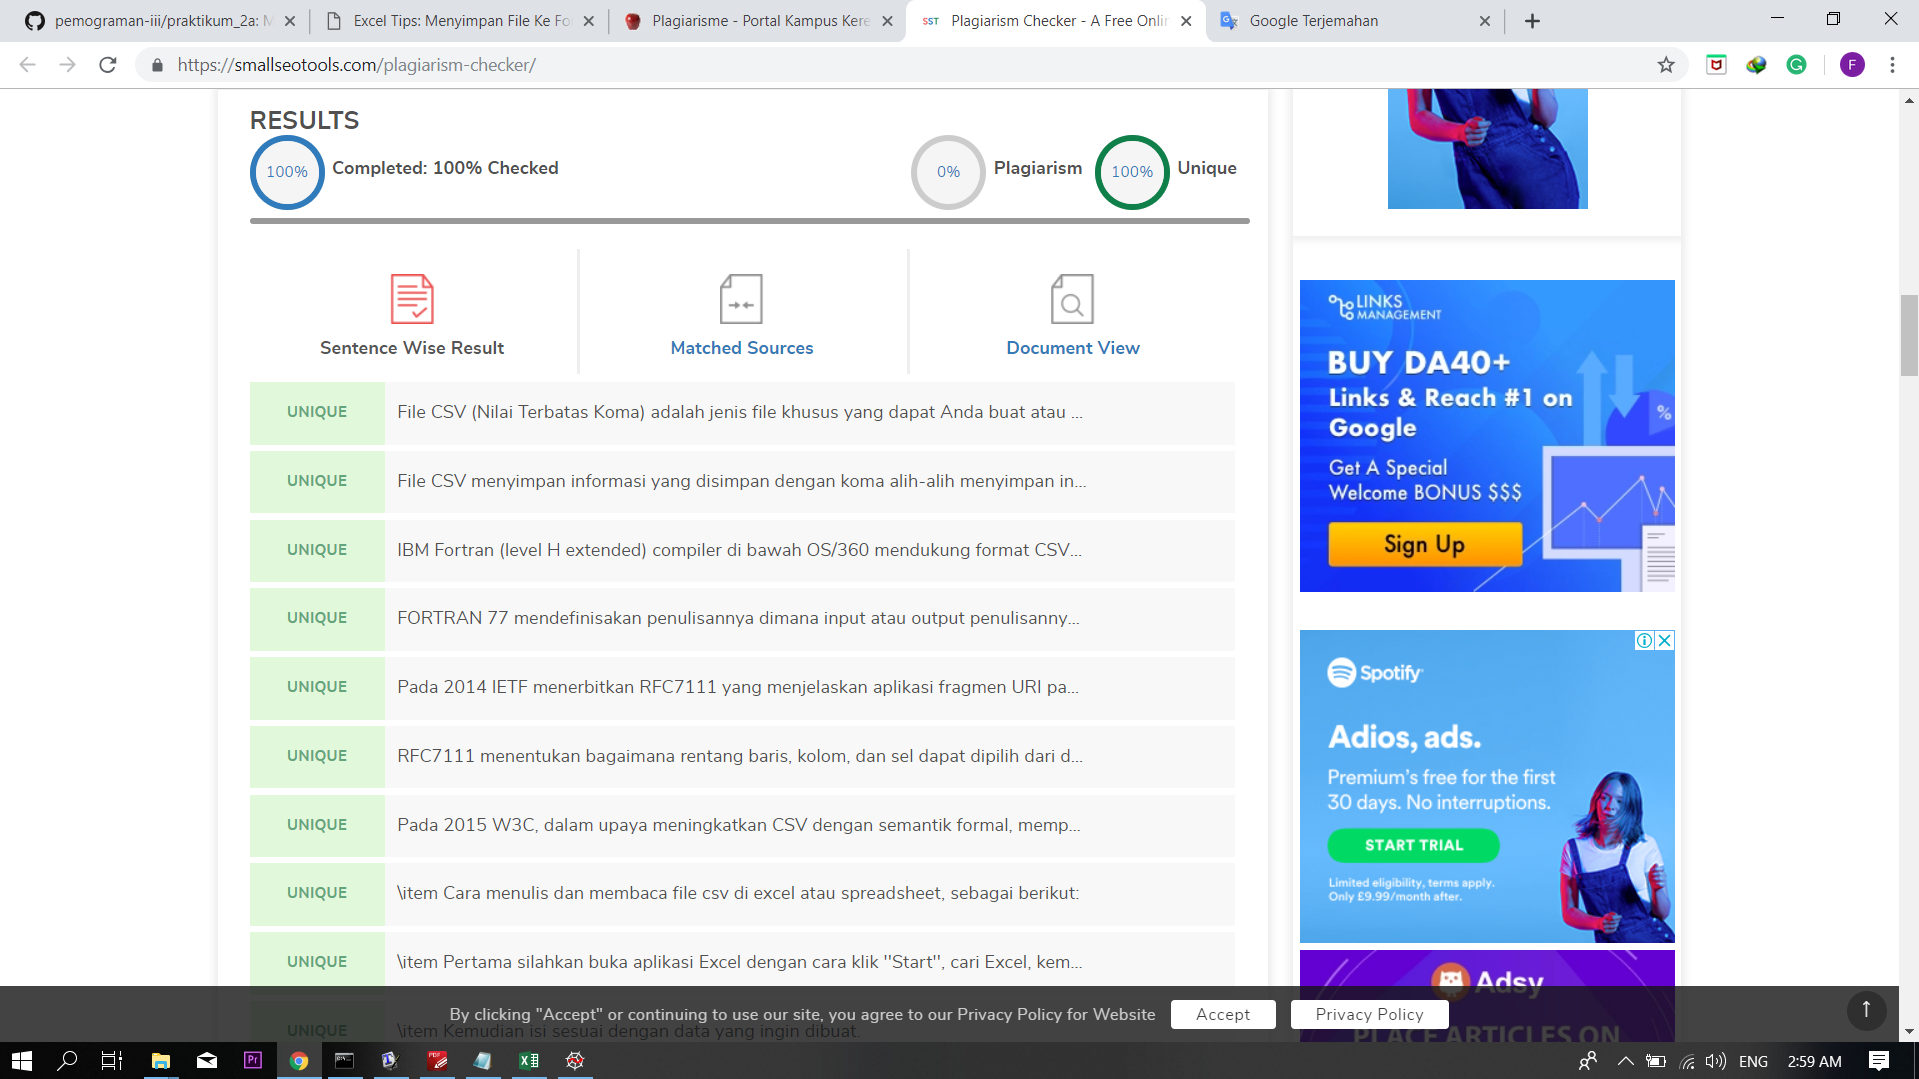
\includegraphics[width=10cm]{figures/4/1174026/Teori/plagiat_teori.png}
	\centering
\end{figure}
%%%%%%%%%%%%%%%%%%%%%%%%%%%%%%%%%%%%%%%%%%%%%

\section{Dwi Septiani Tsaniyah}
\subsection{Soal 1}
\textbf{Pengenalan CSV}

\textbf{Sejarah Format CSV}

File CSV (Nilai Berbatas Koma) adalah tipe file khusus yang dapat Anda buat atau edit di Excel. File CSV menyimpan informasi yang dipisahkan oleh koma, bukan menyimpan informasi dalam kolom. Saat teks dan angka disimpan dalam file CSV, mudah untuk memindahkannya dari satu program ke program lain. Misalnya, Anda dapat mengekspor kontak dari Google ke dalam file CSV, kemudian mengimpornya ke Outlook.
Creating Shared Value (CSV) adalah sebuah konsep dalam strategi bisnis yang menekankan pentingnya memasukkan masalah dan kebutuhan sosial dalam perancangan strategi perusahaan. CSV merupakan pengembangan dari konsep tanggung jawab sosial perusahaan (Corporate social responsibility, CSR). Konsep ini pertama kali diperkenalkan oleh Michael Porter dan Mark Kramer pada tahun 2006. Konsep CSV didasari pada ide adanya hubungan interdependen antara bisnis dan kesejahteraan sosial. Porter mengkritik bahwa selama ini bisnis dan kesejahteraan sosial selalu ditempatkan berseberangan. Pebisnis pun rela mengorbankan kesejahteraan sosial demi keuntungan semata, misalnya dengan melakukan proses produksi yang tidak memperhatikan lingkungan atau menciptakan polusi. CSV menekankan adanya peluang untuk membangun keunggulan kompetitif dengan cara memasukan masalah sosial sebagai bahan pertimbangan utama dalam merancang strategi perusahaan.
contoh : Ketika Toyota memperkenalkan Prius, sebuah kendaraan hybrid listrik/bensin, Toyota berhasil mendapatkan keunggulan kompetitif dengan memasarkan sebuah kendaraan yang tidak hanya memberikan keuntungan ekonomis, namun juga berdampak positif bagi lingkugan. Urbi, sebuah perusahaan konstruksi asal Meksiko, mengembangkan pasar perumahan dengan memberikan kredit murah untuk pekerja dengan gaji kecil, Whole Foods Market telah menjadi pemimpin kategori di segmen supermarket dengan menawarkan makanan organik dan alami kepada konsumen yang sadar lingkungan. Perusahaan juga dapat meningkatkan keunggulan kompetitif dengan melakukan investasi di komunitas di mana mereka beroperasi. Nestlé, misalnya, berhubungan sangat dekat dengan Distrik Susu Moga di India, melakukan investasi pada infrastruktur lokal, dan mentransfer teknologi kelas dunia untuk membangun rantai suplai yang kompetitif sekaligus meningkatkan kesejahteraan sosial melalui peningkatan kesehatan masyarakat, pendidikan yang lebih baik, dan pertumbuhan ekonomi.

\subsection{Soal 2}
Aplikasi-aplikasi yang dapat menciptkan file csv, yaitu:

\begin{itemize}
\item Texteditor , Seperti notepad,visual studio code,atom,sublime dan lain sebagainya
\item Program Spreadsheet , Seperti excell,google spreadshare,LibreOfficecalc
\end{itemize}

\subsection{Soal 3}
\begin{enumerate}
\item Cara menulis dan membaca file csv di excel atau spreadsheet, sebagai berikut:
 Ada dua cara untuk mengimpor data dari file teks dengan Excel dapat membukanya di Excel, atau mengimpornya sebagai rentang data eksternal. Untuk mengekspor data dari Excel menjadi file teks, gunakan perintah Simpan Sebagai dan ubah tipe file dari menu menurun.
\item Ada dua format file teks yang biasanya digunakan:
File teks berbatas (.txt), dengan karakter TAB (kode karakter ASCII 009) yang biasanya memisahkan setiap bidang teks.
File teks nilai yang dipisahkan koma (.csv), dengan karakter koma (,) yang biasanya memisahkan setiap bidang teks.
\end{enumerate}

\subsection{Soal 4}
Sejarah library csv

Library csv mengimplementasikan kelas untuk membaca dan menulis data tabular dalam format CSV. Hal ini memungkinkan programmer untuk mengatakan, "tulis data ini dalam format yang disukai oleh Excel," atau "baca data dari file ini yang dihasilkan oleh Excel," tanpa mengetahui detail yang tepat dari format CSV yang digunakan oleh Excel. Pemrogram juga dapat menggambarkan format CSV yang dipahami oleh aplikasi lain atau menentukan format CSV tujuan khusus mereka sendiri.

\subsection{Soal 5}
Sejarah library pandas

Pada 2008, pengembangan pandas dimulai di AQR Capital Management. Pada akhir 2009 telah menjadi open source, dan secara aktif didukung hari ini oleh komunitas individu yang berpikiran sama di seluruh dunia yang menyumbangkan waktu dan energi berharga mereka untuk membantu membuat panda open source menjadi mungkin.

Sejak 2015, pandas adalah proyek yang disponsori NumFOCUS. Ini akan membantu memastikan keberhasilan pengembangan panda sebagai proyek sumber terbuka kelas dunia.

\subsection{Soal 6}
Fungsi-fungsi yang terdapat di library csv, yaitu:
\begin{enumerate}
	\item reader
	Fungsi ini digunakan untuk membaca isi file berformat CSV dari list.
\end{enumerate}

\subsection{Soal 7}
Jelaskan fungsi-fungsi yang terdapat di library csv
\begin{enumerate}
	\item Terdapat 2 fungsi yang bisa digunakan oleh library csv
	Pertama,fungsi membaca file csv.
\end{enumerate}


\section{Muhammad Fahmi}
\subsection{Soal 1}
Pengenalan CSV

CSV adalah singkatan dari \textit{Comma Separated Value} adalah salah satu tipe file yang digunakan secara luas untuk keperluan programming. Tidak hanya itu, CSV pun sering digunakan dalam pengolahan suatu informasi yang dihasilkan dari spreadsheet yang akan diproses lebih lanjut melalui mesin analitik. CSV juga dianggap sebagai file yang agnostik karena dapat digunakan oleh berbagai database untuk keperluan proses backup data. File CSV sangat mudah untuk dikerjakan secara terprogram. Bahasa apa pun yang mendukung input file teks dan manipulasi string (seperti Python) dapat bekerja dengan file CSV secara langsung.
\textbf{Contoh}
\lstinputlisting[frame=single, caption=Contoh CSV, firstline=1, lastline=13]{src/4/1174021/Teori/1174021.py}

Hasil yang diatas adalah : 
	\begin{figure}[H]
		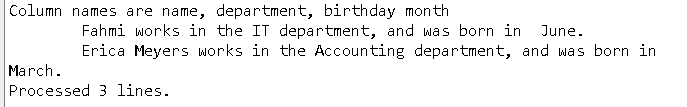
\includegraphics[width=10cm]{figures/4/1174021/Teori/7.png}
		\centering
	\end{figure}

\subsection{Soal 2}
Aplikasi-aplikasi menciptakan file CSV

\begin{itemize}
	\item Text Editor
	Ada beberapa Text Editor untuk menciptakan file CSV diantara lain : 
	\begin{enumerate}
		\item Notepad
		\item Notepad++
		\item Sublime Text
		\item Visual Studio Code
		dll	
	\end{enumerate}

	\item Program Spreadsheet 
	Ada beberapa Program Spreadsheet untuk menciptakan file CSV diantara lain : 
	\begin{enumerate}
		\item Microsoft Excel
		\item WPS
		\item Google Spreadsahre
		\item LibreOfficecalc 
		dll	
	\end{enumerate}
\end{itemize}

\subsection{Soal 3}
Menulis dan membaca file CSV

\begin{enumerate} 
	\item Menulis File CSV \\
	Cara membuat file CSV sederhana yang menulis sejumlah data. Hasilnya akan berupa file CSV di satu tempat dengan file Python, penulis file CSV.
	
	Berikutnya adalah kode untuk menulis file CSV menggunakan modul CSV bawaan yang dimiliki Python:
	
	\lstinputlisting[frame=single, caption=Menulis file CSV, firstline=17, lastline=37]{src/4/1174021/Teori/1174021.py}
	
	Hasil yang diatas adalah : 
	\begin{figure}[H]
		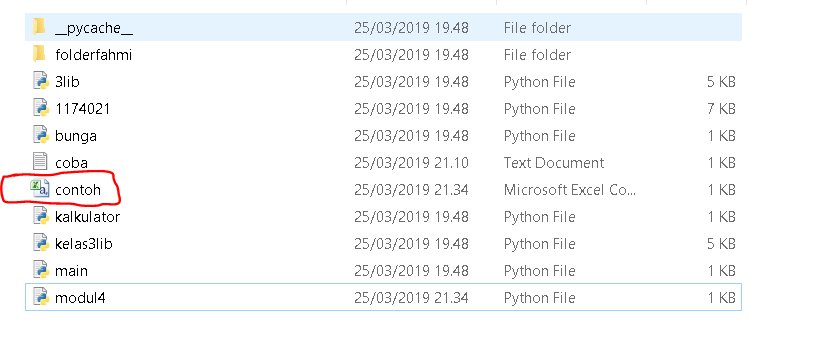
\includegraphics[width=10cm]{figures/4/1174021/Teori/8.png}
		\centering
	\end{figure}

	\item Membaca File CSV \\
	Sekarang kita akan mencoba membaca file CSV yang telah dihasilkan oleh aplikasi atau program lain. Dalam Python, hasil membaca setiap baris dalam file CSV akan dikonversi menjadi daftar Python.
	
	Berikut adalah sebuah kode sederhana untuk membaca file CSV :
	\lstinputlisting[frame=single, caption=Membaca file CSV, firstline=42, lastline=53]{src/4/1174021/Teori/1174021.py}
\end{enumerate}


\subsection{Soal 4}
Sejarah Library CSV

CSV diciptakan untuk memudahkan data science dan analis karena CSV terdapat beberapa kemudahan dalam menggunakannya, CSV dapat dimaksimalkan jika dipadukan dengan Python karena Python adalah salah satu bahasa pemrograman yang bisa support ke banyak library termasuk CSV. Maka CSV menjadi salah satu pilihan yang digunakan oleh perusahaan-perushaan besar dalam mengolah datanya. Library CSV juga dibuat untuk mempermudah jika ingin melakukan export dan import dalam file CSV.

\subsection{Soal 5}
Sejarah Library Pandas

Panda library dibuat agar bahasa pemrograman python dapat bersaing R dan matlab, yang digunakan untuk mengolah banyak data, membutuhkan data besar, data mining data sains dan sebagainya.
panda adalah pustaka berlisensi BSD dan sumber terbuka yang menyediakan struktur data yang mudah digunakan dan berkinerja tinggi serta analisis data untuk bahasa pemrograman Python.
Dengan demikian, Pandas adalah pustaka analisis data yang memiliki struktur data yang kita butuhkan untuk membersihkan data mentah menjadi bentuk yang cocok untuk analisis (mis. Tabel). Penting untuk dicatat di sini bahwa karena melakukan tugas-tugas penting seperti menyinkronkan data untuk perbandingan dan menggabungkan set data, menangani data yang hilang, dll. Pandas awalnya dirancang untuk menangani data keuangan, karena alternatif umum adalah menggunakan spreadsheet (seperti Microsoft Excel).

\subsection{Soal 6}
Jelaskan fungsi-fungsi yang terdapat di library CSV

Ada 2 fungsi yang terdapat pada library CSV yaitu :
\begin{enumerate} 
	\item Menulis File CSV 
	Cara membuat file CSV sederhana yang menulis sejumlah data. Hasilnya akan berupa file CSV di satu tempat dengan file Python, penulis file CSV.
	
	Berikutnya adalah kode untuk menulis file CSV menggunakan modul CSV bawaan yang dimiliki Python:
	
	\lstinputlisting[frame=single, caption=Menulis file CSV, firstline=17, lastline=37]{src/4/1174021/Teori/1174021.py}
	
	Hasil yang diatas adalah : 
	\begin{figure}[H]
		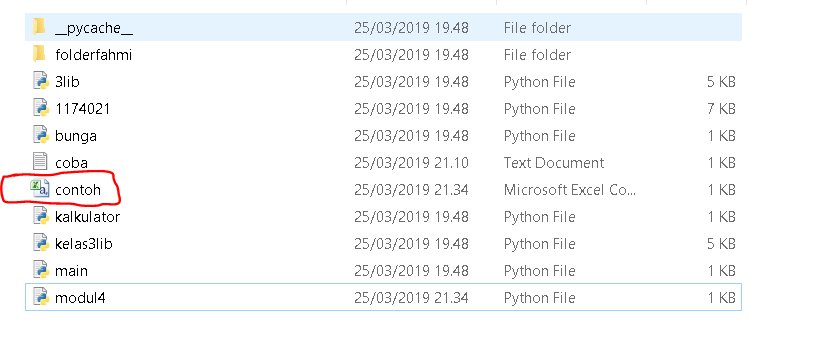
\includegraphics[width=10cm]{figures/4/1174021/Teori/8.png}
		\centering
	\end{figure}
	
	\item Membaca File CSV 
	Sekarang kita akan mencoba membaca file CSV yang telah dihasilkan oleh aplikasi atau program lain. Dalam Python, hasil membaca setiap baris dalam file CSV akan dikonversi menjadi daftar Python. \\
	
	Fungsi ini bisa menggunakan list dan dictionary
	
	\begin{itemize}
		\item Dengan List :
		Berikut adalah sebuah kode sederhana untuk membaca file CSV :
		\lstinputlisting[frame=single, caption=List, firstline=1, lastline=13]{src/4/1174021/Teori/1174021.py}
		
		\item Dengan Dictionary : 
		\lstinputlisting[frame=single, caption=Dictionary, firstline=57, lastline=68]{src/4/1174021/Teori/1174021.py}
		
	\end{itemize}
	
\end{enumerate}

\subsection{Soal 7}
Jelaskan fungsi-fungsi yang terdapat di library pandas.

Tidak jauh berbeda dengan fungsi yang ada pada Library CSV, hanya saja panda lebih mudah, singkat dan lebih rapih. Berikut contohnya :
\lstinputlisting[frame=single, caption=Pandas, firstline=73, lastline=75]{src/4/1174021/Teori/1174021.py}

%%%%%%%%%%%%%%%%%%%%%%%%%%%%%%%%%%%%%%%%%%%%%%%%%%%%%%%%%%%%%%%%%

\section{Muhammad Tomy}
\subsection{Soal 1}
File CSV (Nilai Berbatas Koma) adalah file khusus yang dapat dibuat di Excel. File CSV merupakan file yang menyimpan informasi apapun yang dipisahkan oleh koma. Keunggulan dari file csv adalah mudah untuk memindahkannya. Contohnya, kita bisa melakukan ekspor kontak dari Google ke file CSV, kemudian melanjutkannya mengimpornya ke Outlook.
Nilai yang dipisahkan oleh koma adalah format data yang memberi tanggal lebih awal pada komputer pribadi lebih dari satu dekade, kompiler IBM Fortran (level H extended) di bawah OS / 360 mendukungnya pada tahun 1972. Input / output daftar-diarahkan ("bentuk bebas") didefinisikan dalam FORTRAN 77, disetujui pada tahun 1978. Input yang diarahkan daftar menggunakan koma atau spasi untuk pembatas, sehingga string karakter yang tidak dikutip tidak dapat mengandung koma atau spasi.
Meskipun mendukung format XML baru, Excel 2007 masih mendukung format lama yang masih berbasis BIFF tradisional. Selain itu Microsoft Excel juga mendukung format Comma Separated Values (CSV), DBase File (DBF), SYMbolic LinK (SYLK), Format Interchange Data (DIF) dan banyak format lainnya, termasuk format lembar kerja 1-2 Lotus - 3 (WKS, WK1, WK2, dll.) Dan Quattro Pro.

\subsection{Soal 2}
\textbf{Texteditor}
Seperti notepad++,visual studio code,atom,sublime dan lain sebagainya

\textbf{Program Spreadsheet}
Seperti excell,google spreadshare,LibreOfficecalc

\subsection{Soal 3}
\textbf{Cara Menulis}
Buat dokumen baru di Excel. Tambahkan judul kolom untuk setiap potongan informasi yang ingin dicatat (misalnya nama depan, nama belakang, alamat email, nomor telepon, dan ulang tahun), lalu ketikkan informasi dalam kolom yang sesuai. Pilih File lalu Simpan Sebagai. Gunakan kotak menurun untuk memilih CSV (Berbatas koma) (*.csv), beri nama pada file, lalu pilih Simpan.

\textbf{Cara Membaca}
Klik Data kemudian Get External Data lalu klik From Text. Selanjutya muncul Text Import Wizard, lalu arahkan pada file csv yang ingin anda buka klik Open. Step 1 Pilih Delimited, Kemudian Next (Di sini, bisa juga menentukan baris awal yang akan di import) Step 2 Centrang pada Tab dan Comma (Atau sesuai pengaturan File Anda) lalu Next.

\subsection{Soal 4}
Library csv rancang untuk permudah dalam mengolah data. Dan untuk mempermudah melakukan export dan import file csv tersebut.

\subsection{Soal 5}
Pandas merupakan tool yang dapat digunakan sebagai alat analisis data dan struktur untuk bahasa pemrograman Python. Pandas dapat mengolah data dengan mudah, salah satu fitur yang ada dalam pandas adalah Dataframe. 

\subsection{Soal 6}
Library csv mempunyai keunggulan dibandingkan format data lainnya adalah soal kompatibilitas. File csv dapat digunakan, diolah, diekspor/impor, dan dimodifikasi menggunakan berbagai macam perangkat lunak dan bahasa pemrograman. Pada library csv mempunyai fungsi import dan eksport data yang baik dan bisa digunakan dalam jumlah besar.

\subsection{Soal 7}
Pertama yaitu ada fungsi head dan tail diamana fungsi ini digunakan untuk melihat sample data dan yang kedua ada fungsi add dimana digunakan untuk menambah data.

\subsection{Cek Plagiat}

\begin{figure}[H]
	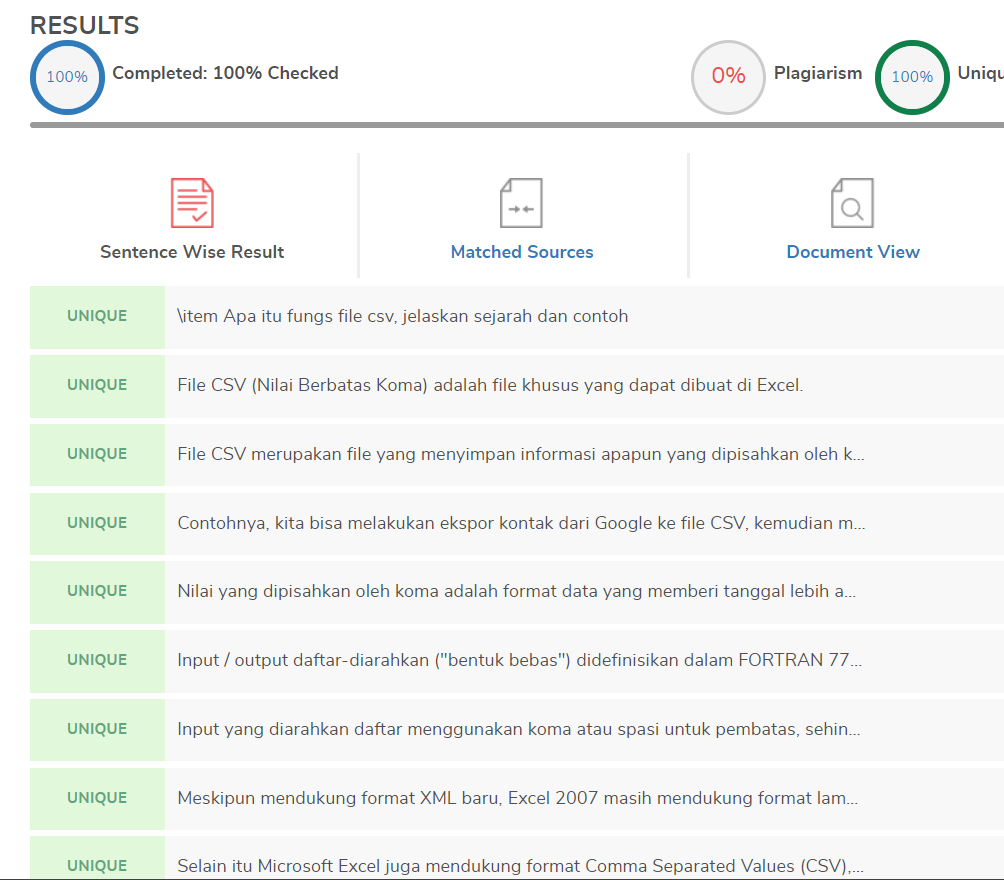
\includegraphics[width=10cm]{figures/4/1174031/Teori/plagiat.png}
	\centering
\end{figure}

%%%%%%%%%%%%%%%%%%%%%%%%%%%%%%%%%%%%%%%%%%%%%%%%%%%


\section{Muh. Rifky Prananda}
\subsection{Apa itu fungsi file csv, jelaskan sejarah dan contoh}
file csv atau nilai terbatas koma adalah suatu jenis file terkhusus yang bisa diedit atau dibuat di excel. file csv sendiri menyimpan sebuah informasi yang terpisahkan oleh koma, dan tidak menyimpan informasi didalam kolom.ketika angka dan teks disimpan didalam file csv, angka dan teks tersebut mudah untuk dipindahkan dari satu program ke program yang lain.
Dari rilis pertama, Excel menggunakan format file biner yang disebut Binary Interchange File Format (BIFF) sebagai format file utamanya. Ini berubah ketika Microsoft merilis Office System 2007 yang memperkenalkan Office Open XML sebagai format file utamanya. Office Open XML adalah file kontainer berbasis XML yang mirip dengan XML Spreadsheets (XMLSS), yang diperkenalkan di Excel 2002. File versi XML tidak bisa menyimpan makro VBA.Meskipun mendukung format XML baru, Excel 2007 masih mendukung format lama yang masih berbasis pada BIFF tradisional. Selain dari yang di atas, Microsoft Excel juga dapat mendukung Comma Separated Values (CSV), DBase Files (DBF), format Data Interchange Data (DIF) dan banyak format lainnya, termasuk lembar kerja 1-2 Lotus- 3 (WKS, WK1, WK2, dll.) Dan Quattro Pro.


\subsection{aplikasi-aplikasi apa saja yang bisa menciptakan file csv }
\begin{itemize}
               \item Program spredsheet
               contohnya seperti google spreadsheet, excel, libreOfficecalc
               \item texteditor
               contohnya seperti sublime, atom, notepad++, visual studio code, dan lain sebagainya.
        \end{itemize}

\subsection{jelaskan bagaimana cara menulis dan membaca file csv di excel atau spreadsheet }
untuk bisa menuliskannya dan dibagian paling atas itu dibuat headernya, untuk lebih mempermudah membedakan datanya, dan untuk baris selanjutnya atau kedua dan seterusnya itu untuk datanya itu sendiri. setelah itu, pilih save as dan pilih format csv. dan untuk membukanya bisa di klik dua kali di file tersebut.

\subsection{ jelaskan sejarah library csv}
 library csv sengaja dibuat untuk memudahkan dalam proses pengelolaan data. dan dapat mempermudah untuk melakukan import dan eksport file csv itu sendiri.

\subsection{ jelaskan sejarah library pandas}
liibrary pandas sengaja dibuat untuk bahasa pemrograman python agar bisa bersaing matlab dan R, yang dapat digunakan untuk mengelola banyak data, keperluan big data, data mining, data sciense dan sebagainya. 

\subsection{jelaskan fungsi-fungsi yang terdapat di library csv}
didalam library csv terdapat 2 fungsi yang bisa digunakan olehnya:
        pertama yaitu fungsi yang bisa membaca sebuah file csv.
        kedua yaitu fungsi yang bisa menulis sebuah file csv.

\subsection{jelaskan fungsi-fungsi yang terdapat di library pandas}
yang pertama yaitu fungsi yang disebut tail dan head yang digunakan untuk melihat sampel data.
        yang kedua yaitu fungsi add yang biasa digunakan untuk menambahkan data. 

\section{Sri Rahayu}
\subsection{Soal 1}
Isi jawaban soal ke-1

Kalau mau dibikin paragrap \textbf{cukup enter aja}, tidak usah pakai \verb|par| dsb

%\subsection{Soal 2}
%Isi jawaban soal ke-2

%\subsection{Soal 3}
%Isi jawaban soal ke-3

\section{Doli Jonviter}
\subsection{Soal 1}
Isi jawaban soal ke-1

Kalau mau dibikin paragrap \textbf{cukup enter aja}, tidak usah pakai \verb|par| dsb

%\subsection{Soal 2}
%Isi jawaban soal ke-2

%\subsection{Soal 3}
%Isi jawaban soal ke-3

\section{Rahmatul Ridha}
\subsection{Soal 1}
Isi jawaban soal ke-1

Kalau mau dibikin paragrap \textbf{cukup enter aja}, tidak usah pakai \verb|par| dsb

%\subsection{Soal 2}
%Isi jawaban soal ke-2

%\subsection{Soal 3}
%Isi jawaban soal ke-3

\section{Tomy Prawoto}
\subsection{Soal 1}
Isi jawaban soal ke-1

Kalau mau dibikin paragrap \textbf{cukup enter aja}, tidak usah pakai \verb|par| dsb

%\subsection{Soal 2}
%Isi jawaban soal ke-2

%\subsection{Soal 3}
%Isi jawaban soal ke-3

%PRAKTEK
\chapter{Praktek Library CSV dan Pandas}
%\section{Kadek Diva Krishna Murti}
\subsection{Soal 1}
Buatlah  fungsi  (file  terpisah/library  dengan  nama  NPMcsv.py)  untuk  membuka file csv dengan lib csv mode list.

\lstinputlisting[caption = Fungsi untuk membuka file CSV dengan lib CSV mode list., firstline=10, lastline=15]{src/4/1174006/Praktek/1174006csv.py}

\subsection{Soal 2}
Buatlah  fungsi  (file  terpisah/library  dengan  nama  NPMcsv.py)  untuk  membuka file csv dengan lib csv mode dictionary.

\lstinputlisting[caption =  Fungsi untuk membuka file CSV dengan lib CSV mode dictionary., firstline=17, lastline=22]{src/4/1174006/Praktek/1174006csv.py}

\subsection{Soal 3}
Buatlah fungsi (file terpisah/library dengan nama NPMpandas.py) untuk membuka file csv dengan lib pandas mode list.

\lstinputlisting[caption =  Fungsi untuk membuka file CSV dengan lib Pandas mode list., firstline=10, lastline=13]{src/4/1174006/Praktek/1174006pandas.py}

\subsection{Soal 4}
Buatlah fungsi (file terpisah/library dengan nama NPMpandas.py) untuk membuka file csv dengan lib pandas mode dictionary.

\lstinputlisting[caption =  Fungsi untuk membuka file CSV dengan lib Pandas mode dictionary., firstline=10, lastline=13]{src/4/1174006/Praktek/1174006pandas.py}

\subsection{Soal 5}
Buat fungsi baru di NPMpandas.py untuk mengubah format tanggal menjadi standar dataframe.

\lstinputlisting[caption =  Fungsi untuk mengubah format tanggal menjadi standar dataframe., firstline=15, lastline=19]{src/4/1174006/Praktek/1174006pandas.py}

\subsection{Soal 6}
Buat fungsi baru di NPMpandas.py untuk mengubah index kolom.

\lstinputlisting[caption =  Fungsi untuk mengubah index kolom., firstline=21, lastline=24]{src/4/1174006/Praktek/1174006pandas.py}

\subsection{Soal 7}
Buat fungsi baru di NPMpandas.py untuk mengubah atribut atau nama kolom.

\lstinputlisting[caption =  Fungsi untuk mengubah atribut atau nama kolom., firstline=26, lastline=30]{src/4/1174006/Praktek/1174006pandas.py}

\subsection{Soal 8}
Buat program main.py yang menggunakan library NPMcsv.py yang membuat dan membaca file csv.

\lstinputlisting[caption =  Membuat dan mebaca file CSV menggunakan library 1174006pandas., firstline=8, lastline=13]{src/4/1174006/Praktek/main.py}

\subsection{Soal 9}
Buat program main2.py yang menggunakan library NPMpandas.py yang membuat dan membaca file csv.

\lstinputlisting[caption = Membuat dan mmebaca file CSV menggunakan library 1174006pandas., firstline=8, lastline=13]{src/4/1174006/Praktek/main2.py}

\subsection{Kode Program Praktek}
\begin{figure}[H]
	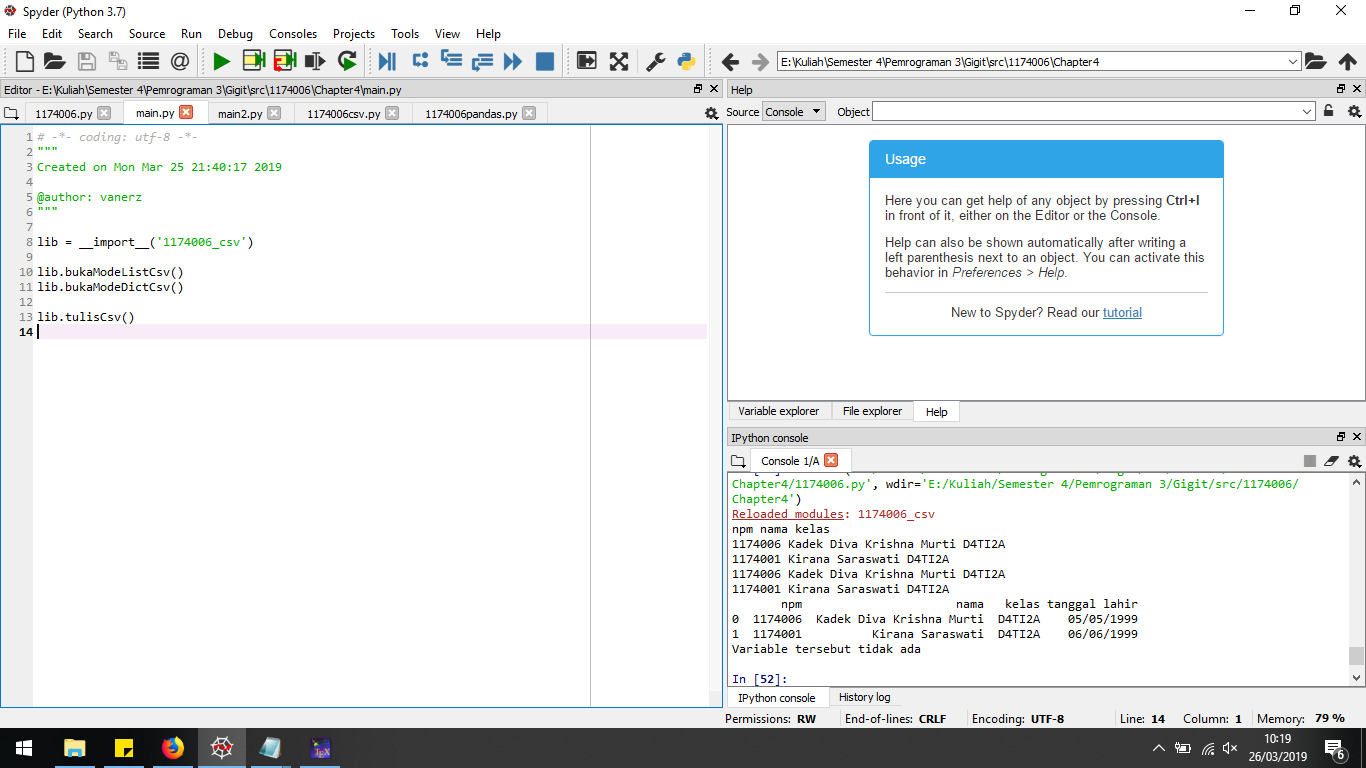
\includegraphics[width=9cm]{figures/4/1174006/Praktek/k1.png}
	\centering
\end{figure}
\begin{figure}[H]
	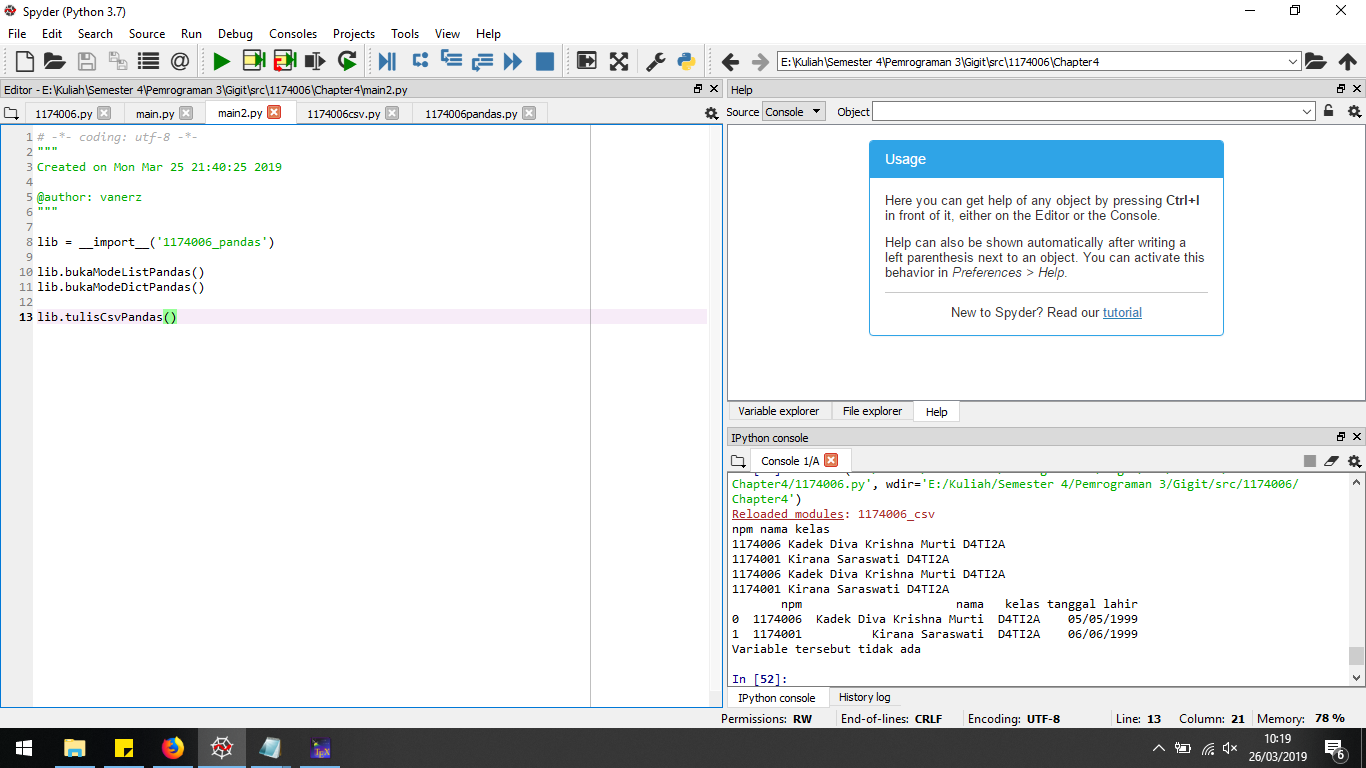
\includegraphics[width=10cm]{figures/4/1174006/Praktek/k2.png}
	\centering
\end{figure}
\begin{figure}[H]
	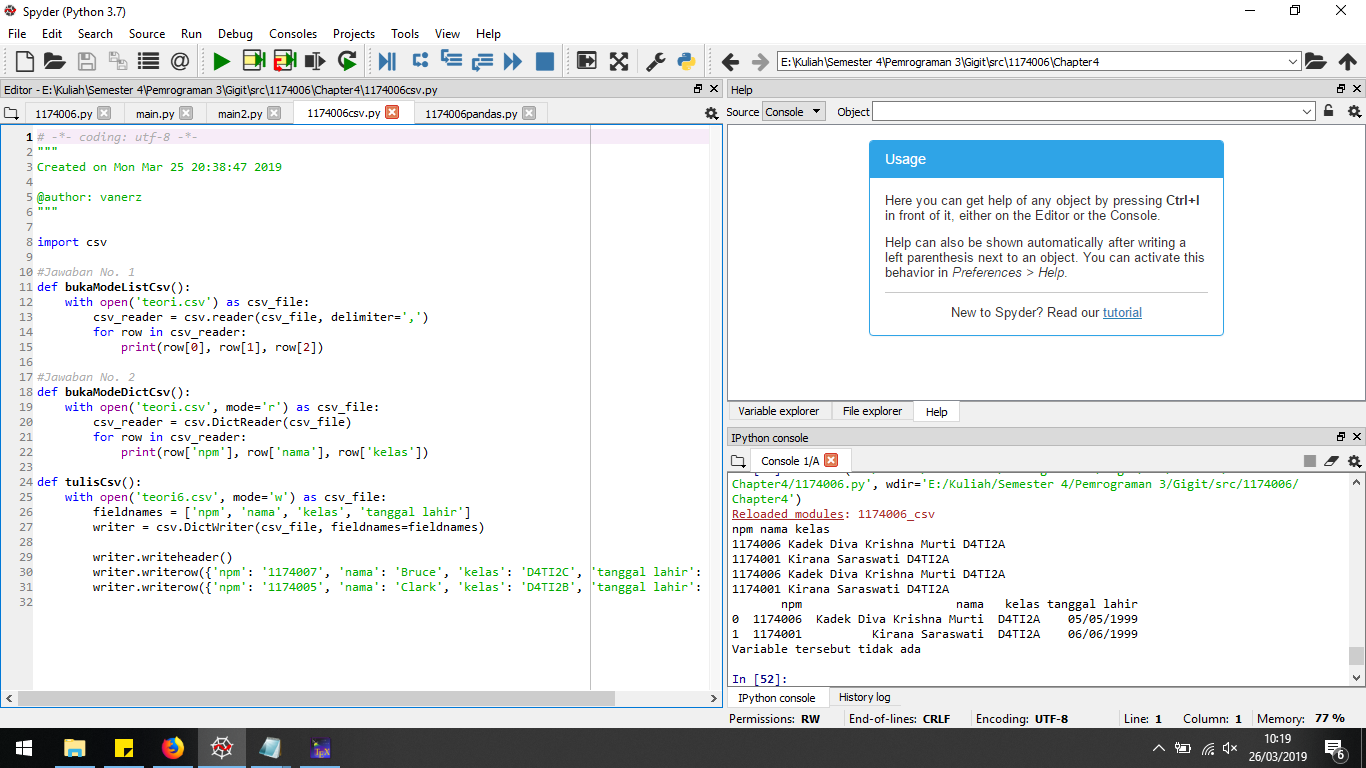
\includegraphics[width=10cm]{figures/4/1174006/Praktek/k3.png}
	\centering
\end{figure}
\begin{figure}[H]
	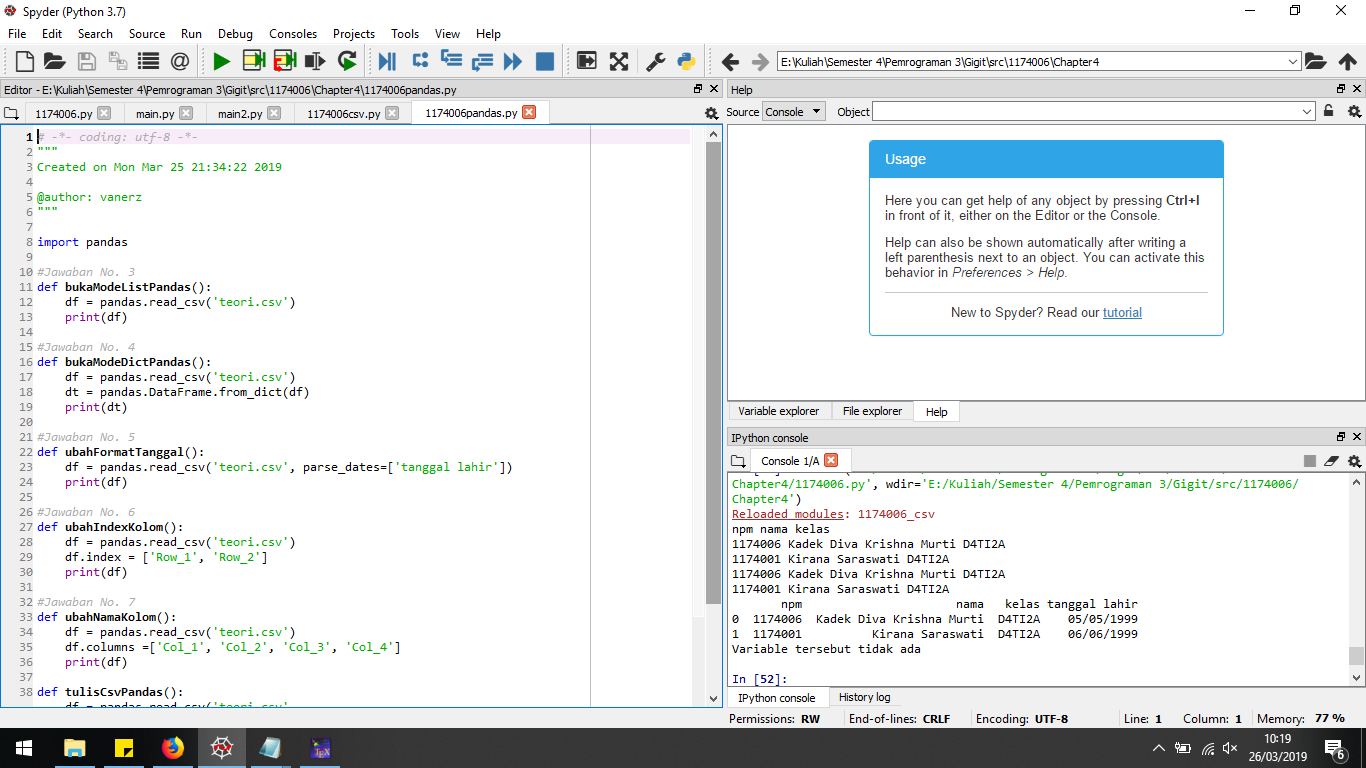
\includegraphics[width=9cm]{figures/4/1174006/Praktek/k4.png}
	\centering
\end{figure}
\begin{figure}[H]
	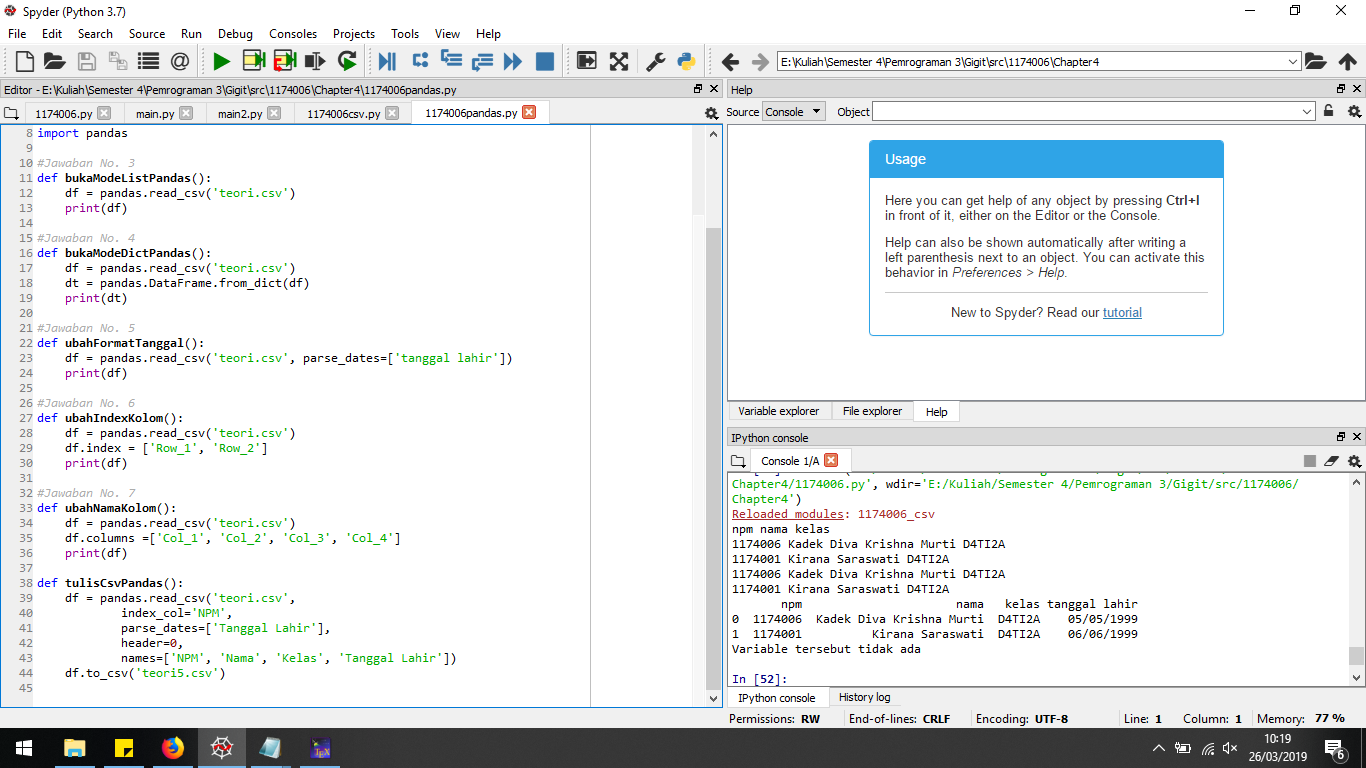
\includegraphics[width=10cm]{figures/4/1174006/Praktek/k5.png}
	\centering
\end{figure}

\subsection{Cek Plagiat Praktek}
\begin{figure}[H]
	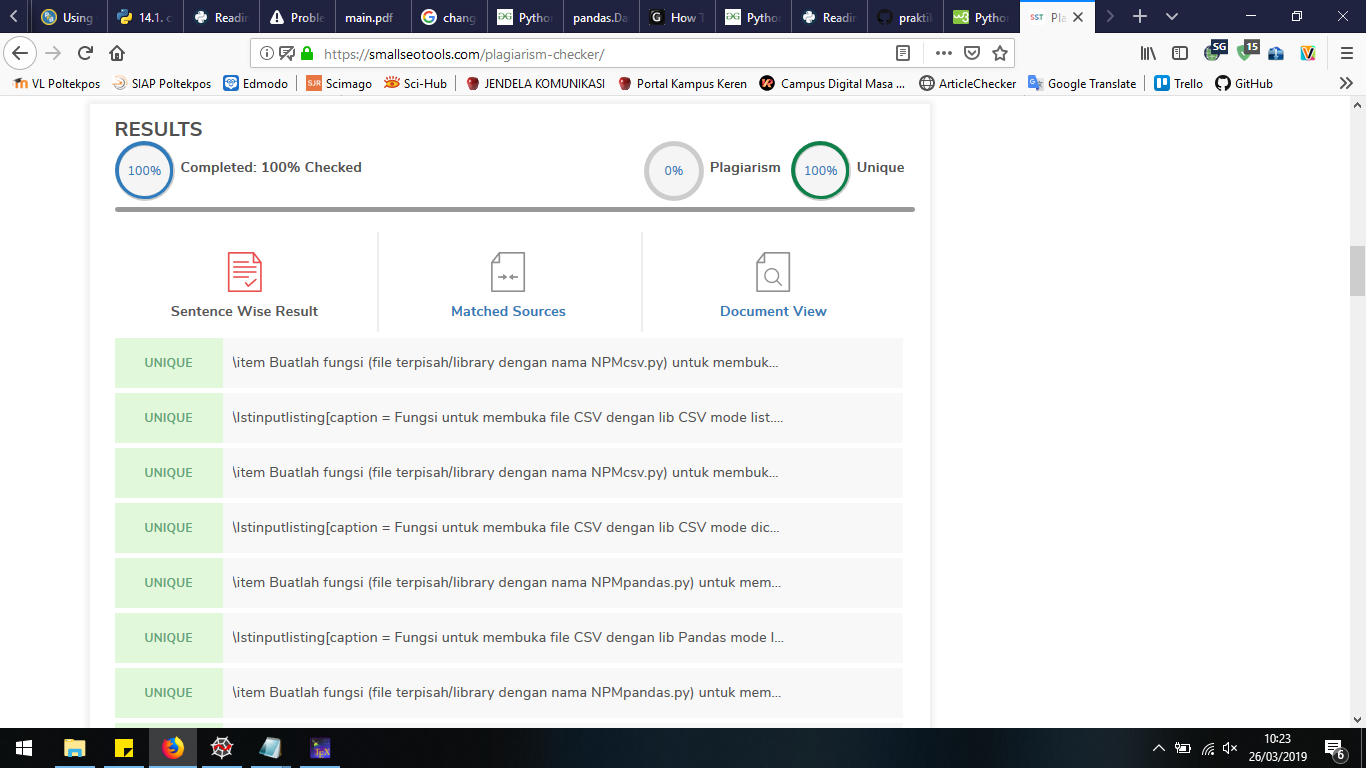
\includegraphics[width=10cm]{figures/4/1174006/Praktek/plagiatketrampilan.png}
	\centering
\end{figure}

\subsection{Soal 1}
Tuliskan  peringatan  error  yang  didapat  dari  mengerjakan  praktek  keempat  ini, dan  jelaskan  cara  penanganan  error  tersebut.   dan  Buatlah  satu  fungsi  yang menggunakan gunakan try except untuk menanggulangi error tersebut.

Peringatan error di praktek keempat ini, yaitu:
\begin{itemize}
	\item Syntax Errors
	Syntax Errors adalah suatu keadaan saat kode python mengalami kesalahan penulisan. Solusinya adalah memperbaiki penulisan kode yang salah.
	
	\item Name Error
	NameError adalah exception yang terjadi saat kode melakukan eksekusi terhadap local name atau global name yang tidak terdefinisi. Solusinya adalah memastikan variabel atau function yang dipanggil ada atau tidak salah ketik.
	
	\item Type Error
	TypeError adalah exception yang akan terjadi apabila pada saat dilakukannya eksekusi terhadap suatu operasi atau fungsi dengan type object yang tidak sesuai. Solusi dari error ini adalah mengkoversi varibelnya sesuai dengan tipe data yang akan digunakan.
\end{itemize}

Fungsi yang menggunakan try except
\lstinputlisting[caption= Fungsi yang menggunakan try except .,firstline=55, lastline=67]{src/4/1174006/Teori/1174006.py}

\subsection{Kode Program Penanganan Error}
\begin{figure}[H]
	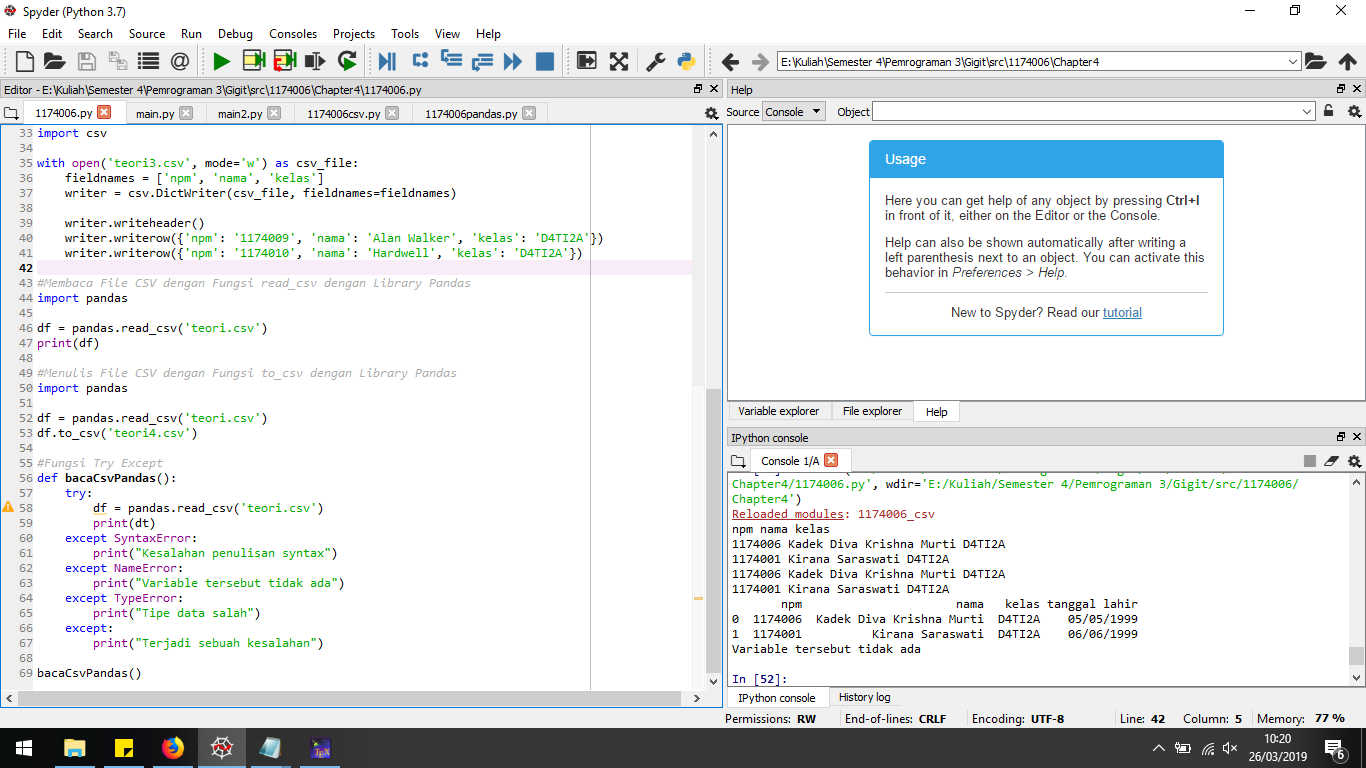
\includegraphics[width=10cm]{figures/4/1174006/Praktek/p1.png}
	\centering
\end{figure}

\subsection{Plagiat Penanganan Error}
\begin{figure}[H]
	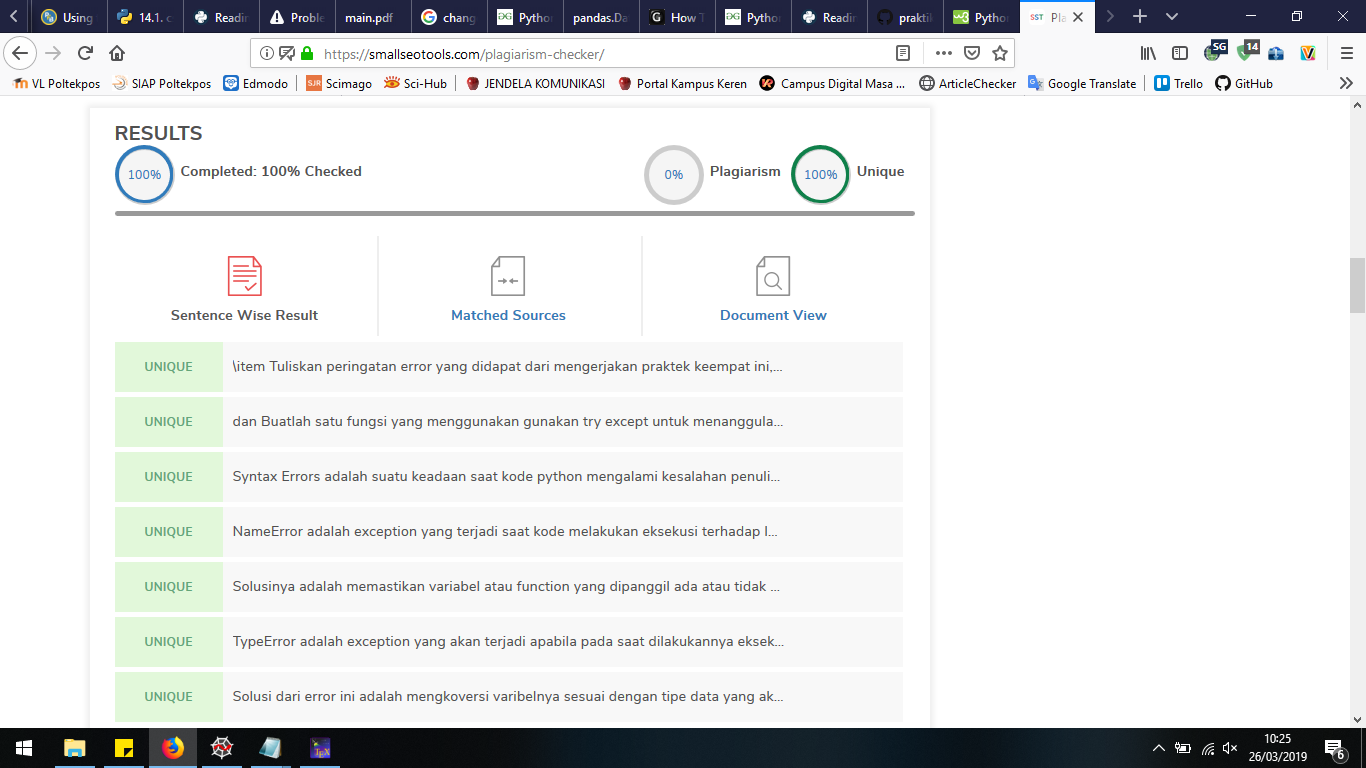
\includegraphics[width=10cm]{figures/4/1174006/Praktek/plagiatpenanganan.png}
	\centering
\end{figure}

%%%%%%%%%%%%%%%%%%%%%%%%%%%%%%%%%%%%%%%%%%%%%%%%%%%%%%%%%%%%%%%%%%%%

\section{Damara Benedikta}
\subsection{Soal 1}
Berikut adalah pemanggilan file csv dengan library csv yang menggunakan list
\lstinputlisting[firstline=10, lastline=20]{src/4/1174012/praktek/c_1174012_csv.py}

\subsection{Soal 2}
Berikut adalah pemanggilan file csv dengan library csv yang menggunakan dictionary
\lstinputlisting[firstline=22, lastline=31]{src/4/1174012/praktek/c_1174012_csv.py}

\subsection{Soal 3}
Berikut adalah pemanggilan file csv dengan library pandas yang menggunakan list
\lstinputlisting[firstline=9, lastline=11]{src/4/1174012/praktek/p_1174012_pandas.py}

\subsection{Soal 4}
Berikut adalah pemanggilan file csv dengan library pandas yang menggunakan dictionary
\lstinputlisting[firstline=13, lastline=16]{src/4/1174012/praktek/p_1174012_pandas.py}

\subsection{Soal 5}
Berikut penggunaan untuk merubah standar penulisan tanggal, yang mengikuti standar penulisan dari pandas.
\lstinputlisting[firstline=18, lastline=20]{src/4/1174012/praktek/p_1174012_pandas.py}

\subsection{Soal 6}
Berikut merupakan pergantian index kolom
\lstinputlisting[firstline=22, lastline=24]{src/4/1174012/praktek/p_1174012_pandas.py}

\subsection{Soal 7}
berikut merupakan penggunaan untuk merename atribut yang digunakan, atau merubah nama header 0
\lstinputlisting[firstline=26, lastline=30]{src/4/1174012/praktek/p_1174012_pandas.py}

\subsection{Soal 8}
\lstinputlisting[firstline=8, lastline=10]{src/4/1174012/praktek/main_damara.py}

\subsection{Soal 9}
\lstinputlisting[firstline=11, lastline=14]{src/4/1174012/praktek/main_damara.py}

\subsection{Penanganan Error}
Tidak ada error
%%%%%%%%%%%%%%%%%%%%%%%%%%%%%%%%%%%%%%%%%%%%%%%%%%%%
\section{Felix Setiawan Lase}
\subsection{Soal 1}
Buatlah  fungsi  (file  terpisah/library  dengan  nama  NPMcsv.py)  untuk  membuka file csv dengan lib csv mode list.

\lstinputlisting[caption = Fungsi untuk membuka file CSV dengan lib CSV mode list., firstline=10, lastline=15]{src/4/1174026/Praktek/1174026_csv.py}

\subsection{Soal 2}
Buatlah  fungsi  (file  terpisah/library  dengan  nama  NPMcsv.py)  untuk  membuka file csv dengan lib csv mode dictionary.

\lstinputlisting[caption =  Fungsi untuk membuka file CSV dengan lib CSV mode dictionary., firstline=17, lastline=22]{src/4/1174026/Praktek/1174026_csv.py}

\subsection{Soal 3}
Buatlah fungsi (file terpisah/library dengan nama NPMpandas.py) untuk membuka file csv dengan lib pandas mode list.

\lstinputlisting[caption =  Fungsi untuk membuka file CSV dengan lib Pandas mode list., firstline=10, lastline=13]{src/4/1174026/Praktek/1174026_pandas.py}

\subsection{Soal 4}
Buatlah fungsi (file terpisah/library dengan nama NPMpandas.py) untuk membuka file csv dengan lib pandas mode dictionary.

\lstinputlisting[caption =  Fungsi untuk membuka file CSV dengan lib Pandas mode dictionary., firstline=10, lastline=13]{src/4/1174026/Praktek/1174026_pandas.py}

\subsection{Soal 5}
Buat fungsi baru di NPMpandas.py untuk mengubah format tanggal menjadi standar dataframe.

\lstinputlisting[caption =  Fungsi untuk mengubah format tanggal menjadi standar dataframe., firstline=15, lastline=19]{src/4/1174026/Praktek/1174026_pandas.py}

\subsection{Soal 6}
Buat fungsi baru di NPMpandas.py untuk mengubah index kolom.

\lstinputlisting[caption =  Fungsi untuk mengubah index kolom., firstline=21, lastline=24]{src/4/1174026/Praktek/1174026_pandas.py}

\subsection{Soal 7}
Buat fungsi baru di NPMpandas.py untuk mengubah atribut atau nama kolom.

\lstinputlisting[caption =  Fungsi untuk mengubah atribut atau nama kolom., firstline=26, lastline=30]{src/4/1174026/Praktek/1174026_pandas.py}

\subsection{Soal 8}
Buat program main.py yang menggunakan library NPMcsv.py yang membuat dan membaca file csv.

\lstinputlisting[caption =  Membuat dan mebaca file CSV menggunakan library 1174006pandas., firstline=8, lastline=13]{src/4/1174026/Praktek/main.py}

\subsection{Soal 9}
Buat program main2.py yang menggunakan library NPMpandas.py yang membuat dan membaca file csv.

\lstinputlisting[caption = Membuat dan mmebaca file CSV menggunakan library 1174006pandas., firstline=8, lastline=13]{src/4/1174026/Praktek/main2.py}

\subsection{Kode Program Praktek}
\begin{figure}[H]
	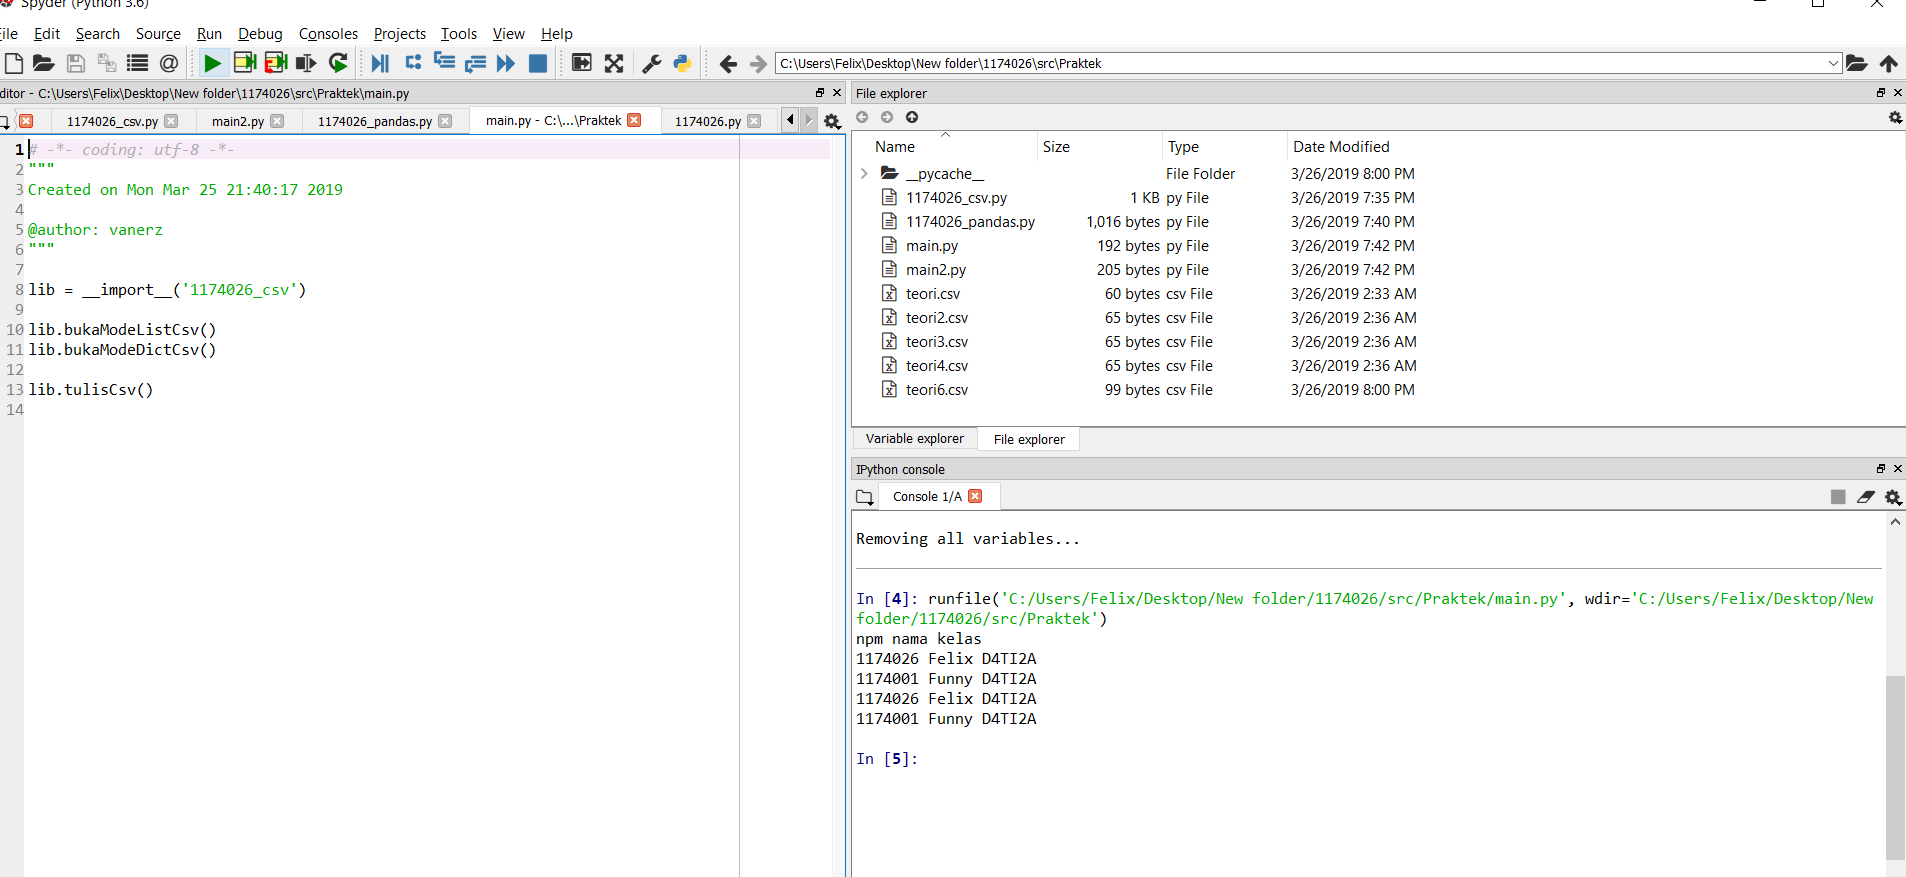
\includegraphics[width=9cm]{figures/4/1174026/Praktek/k1.png}
	\centering
\end{figure}
\begin{figure}[H]
	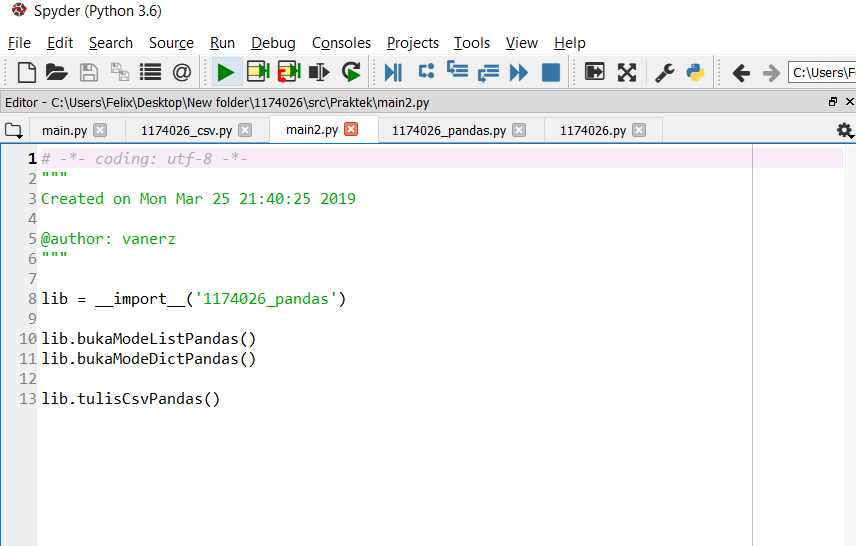
\includegraphics[width=10cm]{figures/4/1174026/Praktek/k2.png}
	\centering
\end{figure}
\begin{figure}[H]
	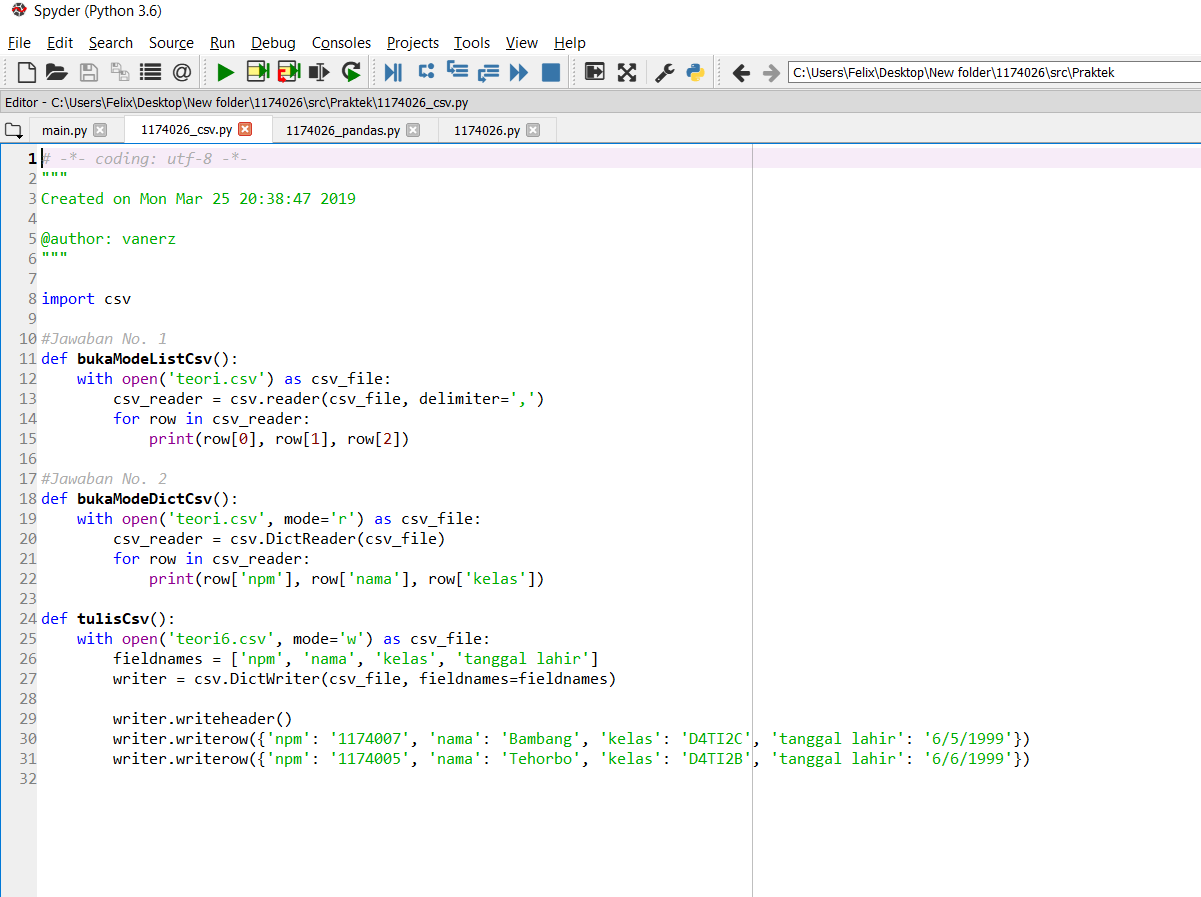
\includegraphics[width=10cm]{figures/4/1174026/Praktek/k3.png}
	\centering
\end{figure}
\begin{figure}[H]
	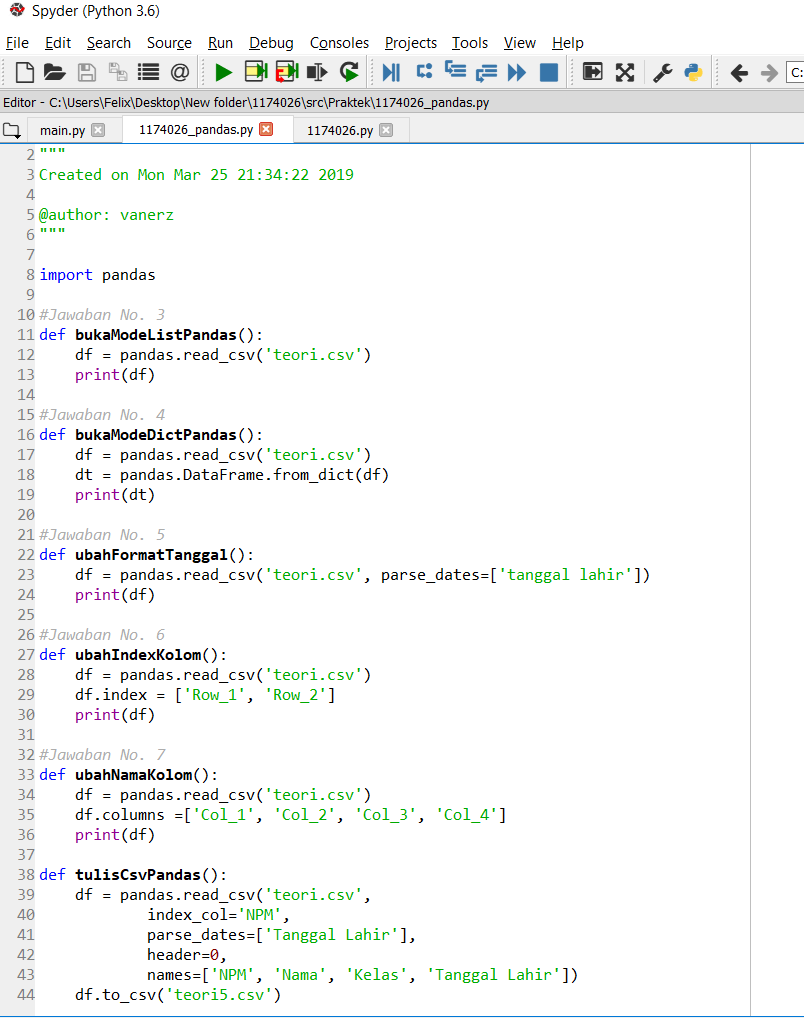
\includegraphics[width=9cm]{figures/4/1174026/Praktek/k4.png}
	\centering
\end{figure}
\begin{figure}[H]
	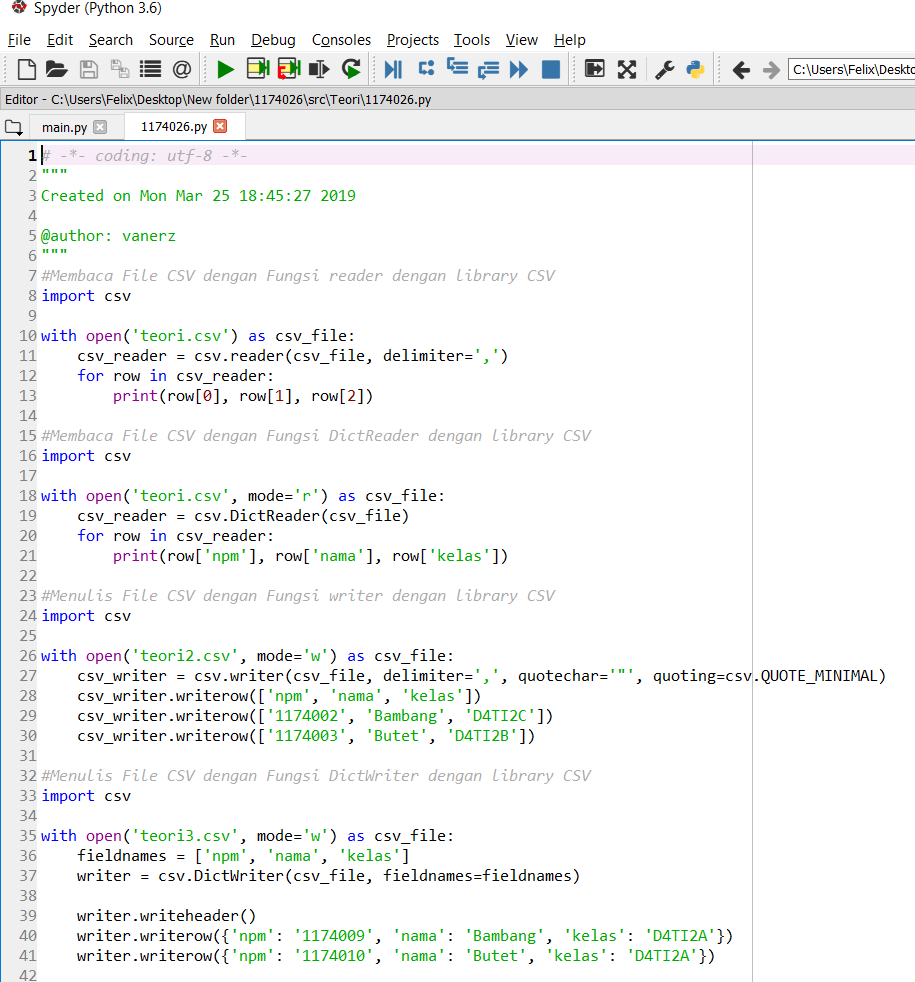
\includegraphics[width=10cm]{figures/4/1174026/Praktek/k5.png}
	\centering
\end{figure}

\subsection{Cek Plagiat Praktek}
\begin{figure}[H]
	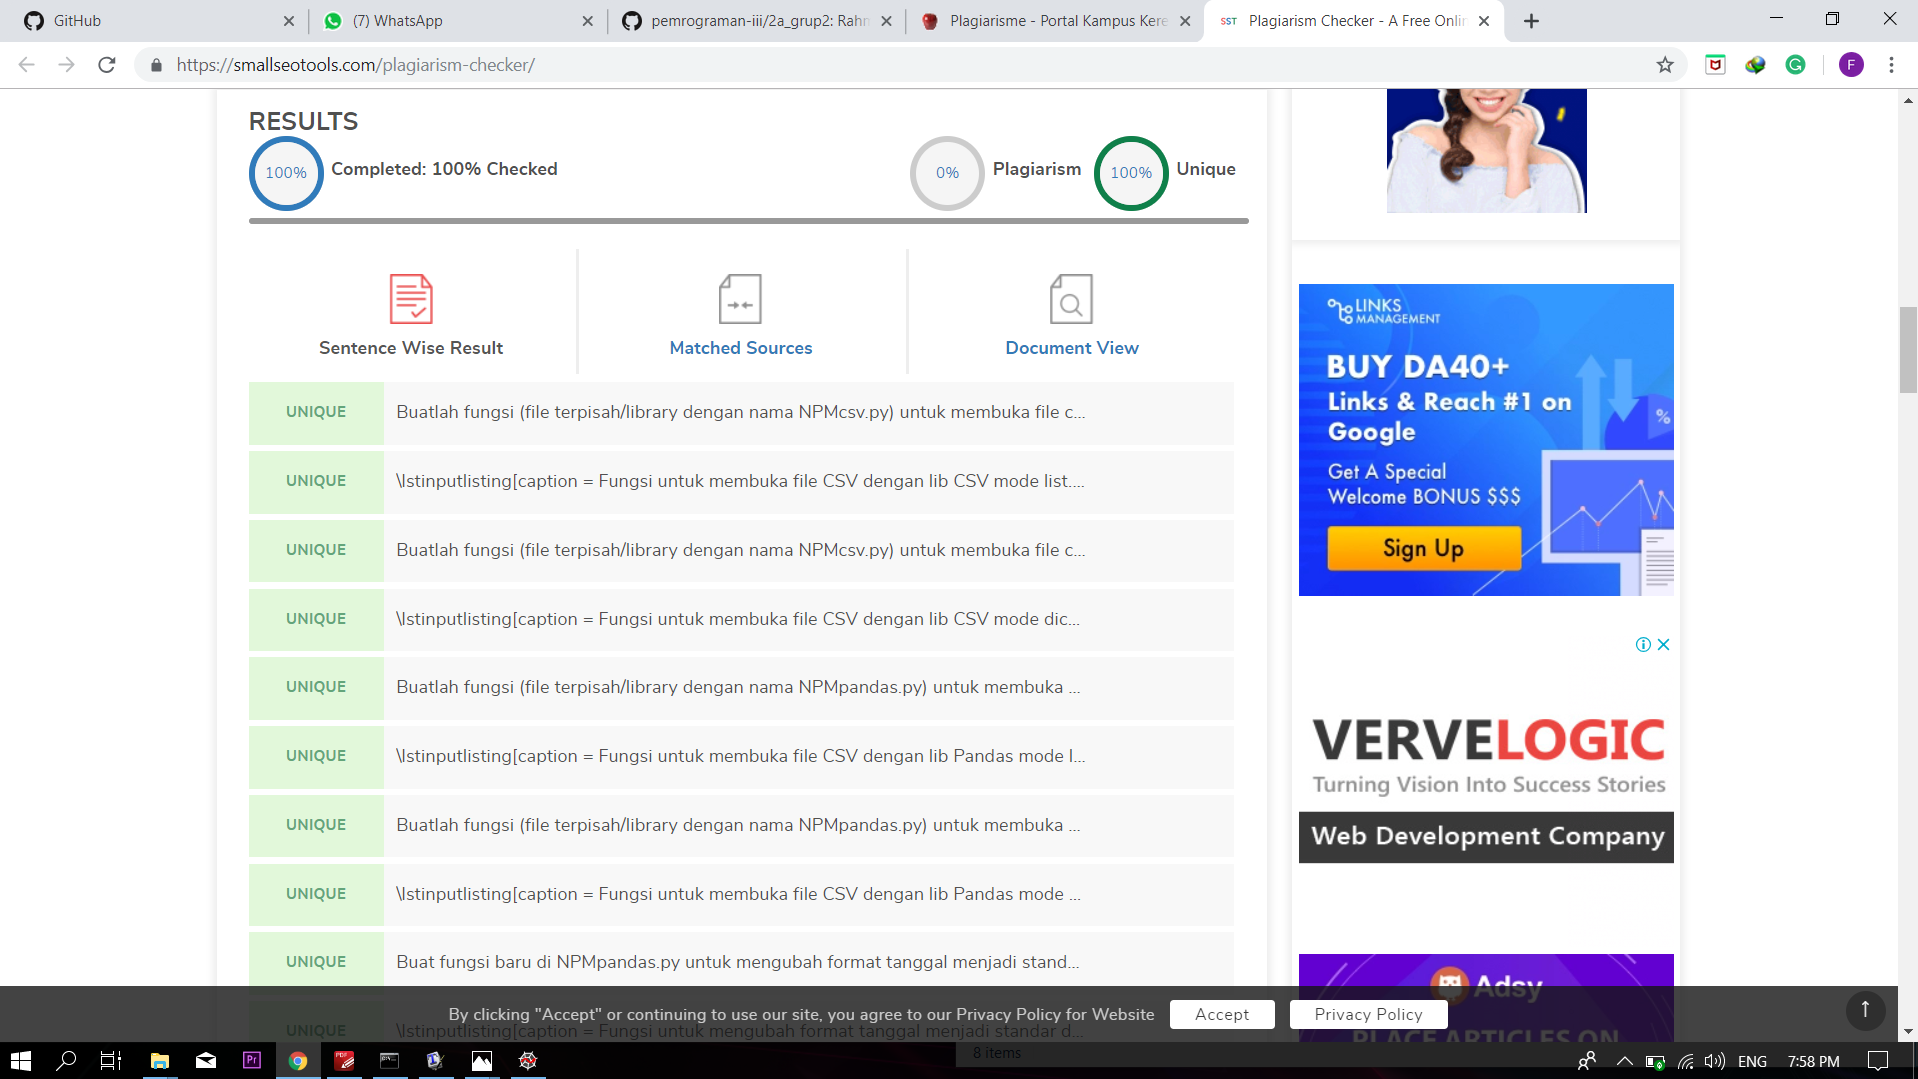
\includegraphics[width=10cm]{figures/4/1174026/Praktek/plagiatketerampilan.png}
	\centering
\end{figure}

\subsection{Soal 1}
Tuliskan  peringatan  error  yang  didapat  dari  mengerjakan  praktek  keempat  ini, dan  jelaskan  cara  penanganan  error  tersebut.   dan  Buatlah  satu  fungsi  yang menggunakan gunakan try except untuk menanggulangi error tersebut.

Peringatan error di praktek keempat ini, yaitu:
\begin{itemize}
	\item Syntax Errors
	Kesalahan Sintaksis adalah suatu kondisi ketika kode python mengalami kesalahan penulisan. Solusinya adalah memperbaiki penulisan kode yang salah.
	
	\item Name Error
	NameError adalah pengecualian yang terjadi ketika kode mengeksekusi nama lokal atau nama global yang tidak ditentukan. Solusinya adalah memastikan variabel atau fungsi yang dipanggil ada atau tidak salah ketik.
	
	\item Type Error
	TypeError adalah pengecualian yang akan terjadi jika eksekusi operasi atau fungsi dengan tipe objek tidak sesuai ketika dieksekusi. Solusi untuk kesalahan ini adalah mengubah variabel sesuai dengan tipe data yang akan digunakan.
\end{itemize}

Fungsi yang menggunakan try except
\lstinputlisting[caption= Fungsi yang menggunakan try except .,firstline=55, lastline=67]{src/4/1174006/Teori/1174026.py}

\subsection{Kode Program Penanganan Error}
\begin{figure}[H]
	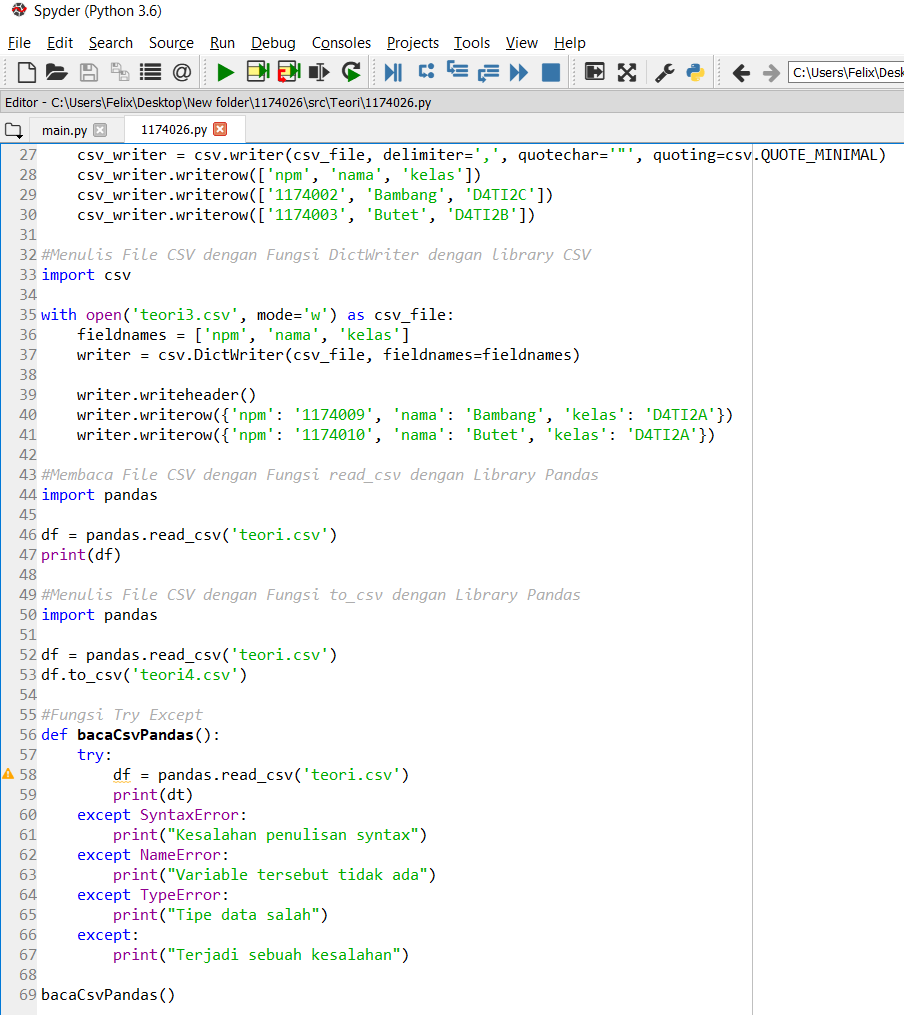
\includegraphics[width=10cm]{figures/4/1174026/Praktek/p1.png}
	\centering
\end{figure}

\subsection{Plagiat Penanganan Error}
\begin{figure}[H]
	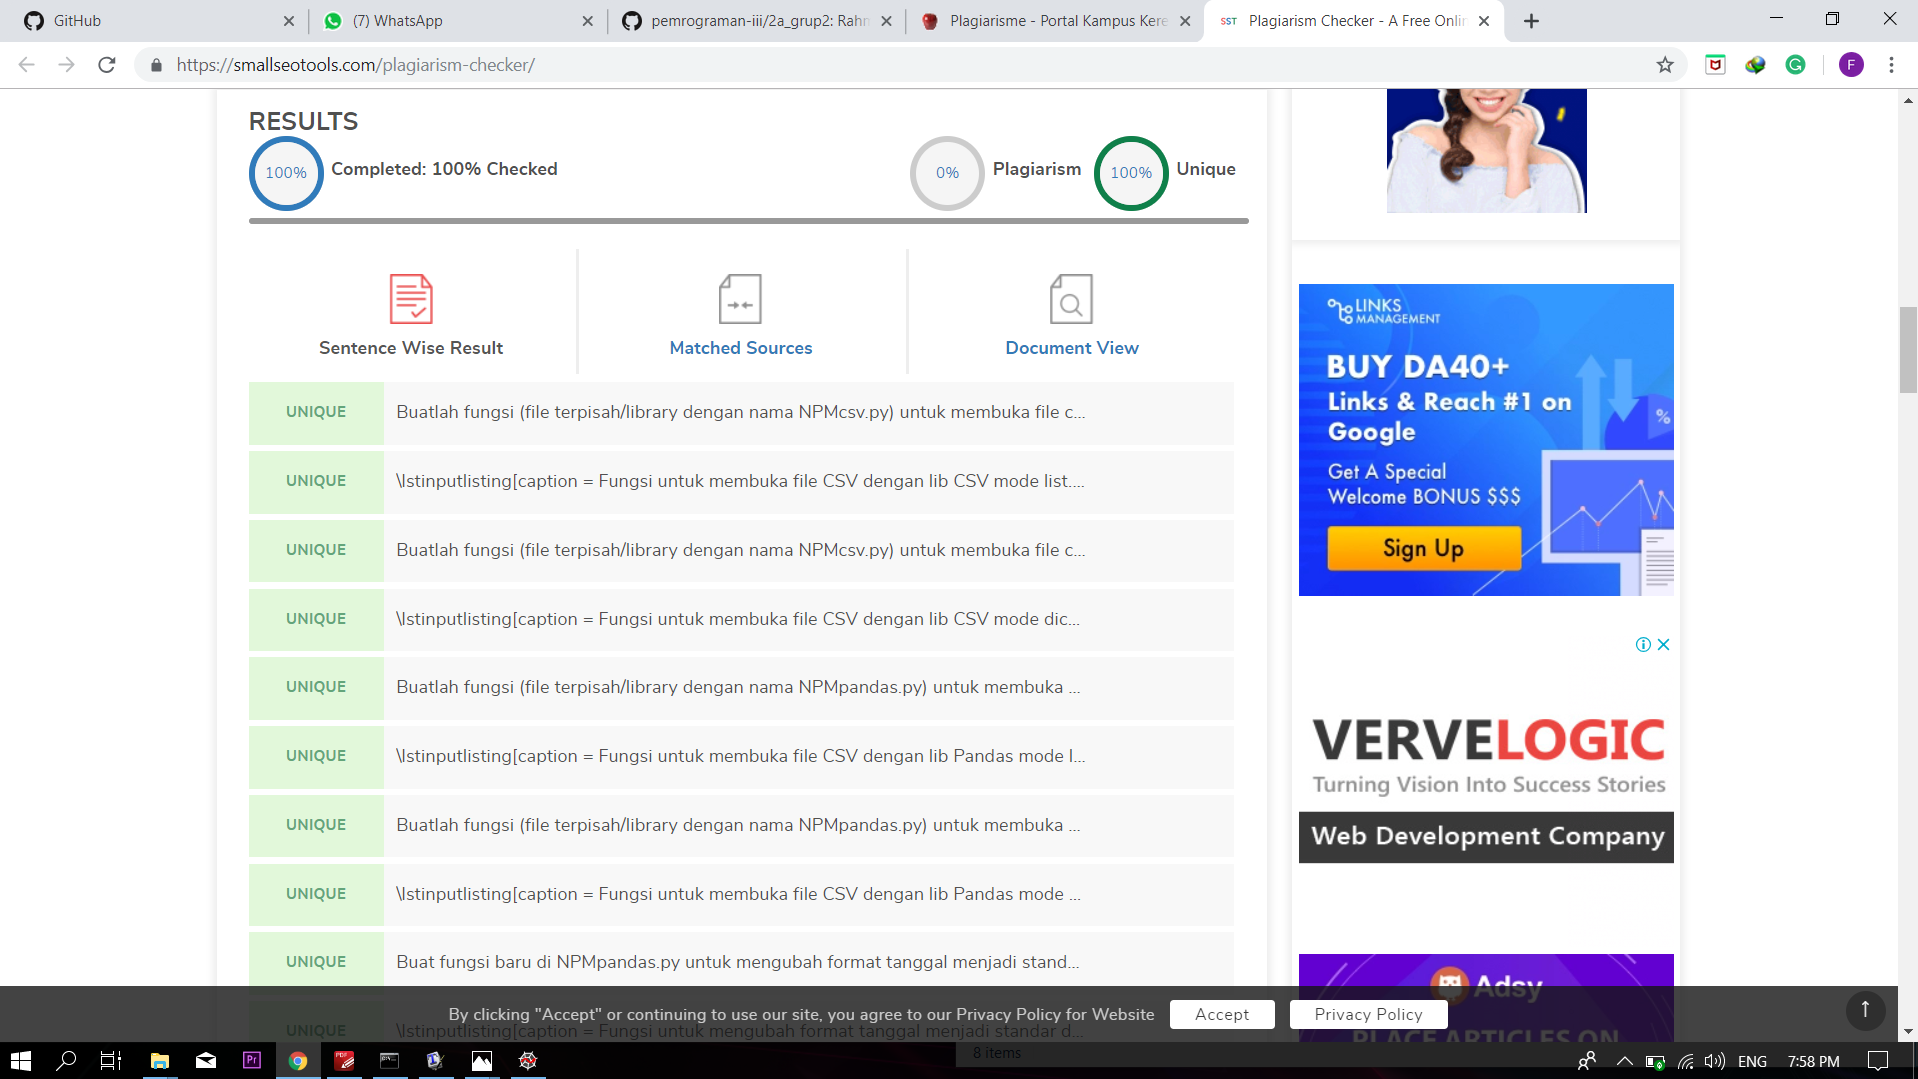
\includegraphics[width=10cm]{figures/4/1174026/Praktek/plagiatpenanganan.png}
	\centering
\end{figure}

%%%%%%%%%%%%%%%%%%%%%%%%%%%%%%%%%%%%%%%%%%%%%%%%%%%%

\section{Dwi Septiani Tsaniyah}
\subsection{Soal 1}
Buatlah  fungsi  (file  terpisah/library  dengan  nama  NPMcsv.py)  untuk  membuka file csv dengan lib csv mode list.
\lstinputlisting[firstline=9, lastline=21]{src/4/1174003/c_1174003_csv.py}

\subsection{Soal 2}
Buatlah  fungsi  (file  terpisah/library  dengan  nama  NPMcsv.py)  untuk  membuka file csv dengan lib csv mode dictionary.
\lstinputlisting[firstline=24, lastline=47]{src/4/1174003/c_1174003_csv.py}

\subsection{Soal 3}
Buatlah fungsi (file terpisah/library dengan nama NPMpandas.py) untuk membuka file csv dengan lib pandas mode list.
\lstinputlisting[firstline=10, lastline=11]{src/4/1174003/p_1174003_pandas.py}

\subsection{Soal 4}
Buatlah fungsi (file terpisah/library dengan nama NPMpandas.py) untuk membuka file csv dengan lib pandas mode dictionary.
\lstinputlisting[firstline=14, lastline=16]{src/4/1174003/p_1174003_pandas.py}

\subsection{Soal 5}
Buat fungsi baru di NPMpandas.py untuk mengubah format tanggal menjadi standar dataframe.
\lstinputlisting[firstline=19, lastline=20]{src/4/1174003/p_1174003_pandas.py}

\subsection{Soal 6}
Buat fungsi baru di NPMpandas.py untuk mengubah index kolom.
\lstinputlisting[firstline=23, lastline=24]{src/4/1174003/p_1174003_pandas.py}

\subsection{Soal 7}
Buat fungsi baru di NPMpandas.py untuk mengubah atribut atau nama kolom.
\lstinputlisting[firstline=27, lastline=42]{src/4/1174003/p_1174003_pandas.py}

\subsection{Soal 8}
Buat program main.py yang menggunakan library NPMcsv.py yang membuat dan membaca file csv.
\lstinputlisting[firstline=8, lastline=10]{src/4/1174003/main_dwi.py}

\subsection{Soal 9}
Buat program main2.py yang menggunakan library NPMpandas.py yang membuat dan membaca file csv.
\lstinputlisting[firstline=12, lastline=14]{src/4/1174003/main_dwi.py}

\subsection{Soal 1}
Tuliskan  peringatan  error  yang  didapat  dari  mengerjakan  praktek  keempat  ini, dan  jelaskan  cara  penanganan  error  tersebut.   dan  Buatlah  satu  fungsi  yang menggunakan gunakan try except untuk menanggulangi error tersebut.

Peringatan error di praktek keempat ini, yaitu:
\begin{itemize}
	\item Syntax Errors
	Syntax Errors adalah suatu keadaan saat kode python mengalami kesalahan penulisan. Solusinya adalah memperbaiki penulisan kode yang salah.
	
	\item Name Error
	NameError adalah exception yang terjadi saat kode melakukan eksekusi terhadap local name atau global name yang tidak terdefinisi. Solusinya adalah memastikan variabel atau function yang dipanggil ada atau tidak salah ketik.
	
	\item Type Error
	TypeError adalah exception yang akan terjadi apabila pada saat dilakukannya eksekusi terhadap suatu operasi atau fungsi dengan type object yang tidak sesuai. Solusi dari error ini adalah mengkoversi varibelnya sesuai dengan tipe data yang akan digunakan.
\end{itemize}

\section{Harun Ar-Rasyid}
\subsection{Soal 1}
Isi jawaban soal ke-1

Kalau mau dibikin paragrap \textbf{cukup enter aja}, tidak usah pakai \verb|par| dsb

%\subsection{Soal 2}
%Isi jawaban soal ke-2

%\subsection{Soal 3}
%Isi jawaban soal ke-3

\section{Sri Rahayu}
\subsection{Soal 1}
Isi jawaban soal ke-1

Kalau mau dibikin paragrap \textbf{cukup enter aja}, tidak usah pakai \verb|par| dsb

%\subsection{Soal 2}
%Isi jawaban soal ke-2

%\subsection{Soal 3}
%Isi jawaban soal ke-3

\section{Doli Jonviter}
\subsection{Soal 1}
Isi jawaban soal ke-1

Kalau mau dibikin paragrap \textbf{cukup enter aja}, tidak usah pakai \verb|par| dsb

%\subsection{Soal 2}
%Isi jawaban soal ke-2

%\subsection{Soal 3}
%Isi jawaban soal ke-3

\section{Rahmatul Ridha}
\subsection{Soal 1}
Isi jawaban soal ke-1

Kalau mau dibikin paragrap \textbf{cukup enter aja}, tidak usah pakai \verb|par| dsb

%\subsection{Soal 2}
%Isi jawaban soal ke-2

%\subsection{Soal 3}
%Isi jawaban soal ke-3

\section{Tomy Prawoto}
\subsection{Soal 1}
Isi jawaban soal ke-1

Kalau mau dibikin paragrap \textbf{cukup enter aja}, tidak usah pakai \verb|par| dsb

%\subsection{Soal 2}
%Isi jawaban soal ke-2

%\subsection{Soal 3}
%Isi jawaban soal ke-3


%TEORI
\chapter{PySerial}
%\section{Kadek Diva Krishna Murti}
{\Large \textbf{Pemahaman Teori}}
\subsection{Soal No. 1}
Apa itu fungsi device manager di windows dan folder /dev di linux?

\hfill \break
Device manager merupakan perangkat lunak untuk menampilkan seluruh perangkat keras yang di-inisialisasi atau dikenali oleh sistem operasi Windows. Device Manager membantu dalam mengelola atau me-manage semua perangkat keras yang terpasang dan terdeteksi dalam sistem Windows. Perangkat keras tersebut bisa berupa harddisk, kartu VGA, sound, keyboard, perangkat USB dan lain-lainnya.

\hfill \break
Fungsi device manager antara lain :
\begin{enumerate}
	\item Menunjukkan status mengenai suatu perangkat keras.
	\item Menunjukkan informasi detail mengenai suatu perangkat keras.
	\item Mengelola driver perangkat keras.
	\item Menonaktifkan dan mengaktifkan perangkat keras.
	\item Mengidentifikasi konflik antar perangkat keras.
	\item Memberitahukan terjadinya masalah pada perangkat keras.
\end{enumerate}

\hfill \break
Folder /dev merupakan representasi dari drive yang terhubung ke sistem operasi Linux dan oleh sistem dianggap sebagai file-file direktori. Biasanya sering ditampilkan direktori seperti /dev/sda1 yang mewakili Drive SATA pertama dalam sistem.

\subsection{Soal No. 2}
Jelaskan langkah-langkah instalasi driver dari arduino!

\hfill \break
Berikut ini adalah langkah-langkah instalasi driver dari Arduino UNO di Windows:

\begin{enumerate}
	\item Pertama pastikan Arduino IDE telah terinstall.
	\item Lalu hubungkan port USB Arduino Uno ke port USB PC.
	\item Kemudian PC anda akan mendeteksi perangkat baru yang terpasang dan akan muncul pop seperti ini.
	\begin{figure}[H]
		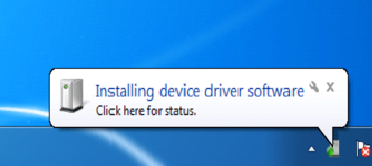
\includegraphics[width=10cm]{figures/5/1174006/Teori/1.png}
		\centering
	\end{figure}
	\item Karena Arduino Uno baru pertama kali terpasang, maka akan muncul pop up error seperti ini.
	\begin{figure}[H]
		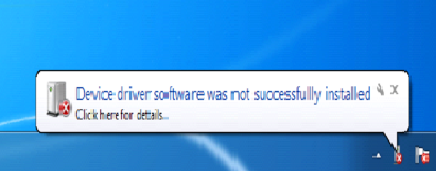
\includegraphics[width=10cm]{figures/5/1174006/Teori/2.png}
		\centering
	\end{figure}
	\item Buka ''Start'' lalu cari Device Manager, kemudian klik ''Device Manager''.
	\begin{figure}[H]
		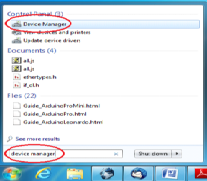
\includegraphics[width=10cm]{figures/5/1174006/Teori/3.png}
		\centering
	\end{figure}
	\item Setelah Device Manager terbuka, silahkan cari ''Unknown Device'' yang berada di Other Device.
	\begin{figure}[H]
		\includegraphics[width=10cm]{figures/5/1174006/Teori/4.png}
		\centering
	\end{figure}
	\item Kemudian klik kanan pada ''Unknown Device'', lalu pilih ''Update Driver Software''.
	\begin{figure}[H]
		\includegraphics[width=10cm]{figures/5/1174006/Teori/5.png}
		\centering
	\end{figure}
	\item Setelah itu muncul window baru, lalu pilih ''Browse my computer for driver software''.
	\begin{figure}[H]
		\includegraphics[width=10cm]{figures/5/1174006/Teori/6.png}
		\centering
	\end{figure}
	\item Lalu cari folder yang terinstall Arduino IDE dengan mengklik browse. Kemudian klik ''Next''.
	\begin{figure}[H]
		\includegraphics[width=10cm]{figures/5/1174006/Teori/7.png}
		\centering
	\end{figure}
	\item Windows akan mencari dan menginstall driver yang berada pada folder tersebut.
	\begin{figure}[H]
		\includegraphics[width=10cm]{figures/5/1174006/Teori/8.png}
		\centering
	\end{figure}
	\item Setelah itu akan muncul window, lalu klik ''Install''.
	\begin{figure}[H]
		\includegraphics[width=10cm]{figures/5/1174006/Teori/9.png}
		\centering
	\end{figure}
	\item Jika berhasil terinstal maka akan muncul window seperti ini.
	\begin{figure}[H]
		\includegraphics[width=10cm]{figures/5/1174006/Teori/10.png}
		\centering
	\end{figure}
\end{enumerate}

\subsection{Soal No. 3}
Jelaskan bagaimana cara membaca baudrate dan port dari komputer yang sudah terinstall driver!

\hfill \break
\textbf{Membaca Baudrate dari Komputer}
\begin{enumerate}
	\item Pertama buka ''Start''. Cari ''Device Manager'', lalu klik.
	\begin{figure}[H]
		\includegraphics[width=10cm]{figures/5/1174006/Teori/d1.png}
		\centering
	\end{figure}
	
	\item Kemudian pilih ''Ports (COM \& LPT)''.
	\begin{figure}[H]
		\includegraphics[width=10cm]{figures/5/1174006/Teori/d3.png}
		\centering
	\end{figure}
	
	\item Klik dua kali pada COM yang terhubung.
	\begin{figure}[H]
		\includegraphics[width=10cm]{figures/5/1174006/Teori/d2.png}
		\centering
	\end{figure}

	\item Pilih tab ''Port Settings'', lalu lihat di ''Bit per second''.
	\begin{figure}[H]
		\includegraphics[width=8cm]{figures/5/1174006/Teori/d4.png}
		\centering
	\end{figure}
\end{enumerate}


\hfill \break
\textbf{Membaca Port dari Komputer}

\begin{enumerate}
	\item Pertama buka ''Start''. Cari ''Device Manager'', lalu klik.
	\begin{figure}[H]
		\includegraphics[width=10cm]{figures/5/1174006/Teori/d1.png}
		\centering
	\end{figure}

	\item Kemudian pilih ''Ports (COM \& LPT)''.
	\begin{figure}[H]
		\includegraphics[width=10cm]{figures/5/1174006/Teori/d3.png}
		\centering
	\end{figure}

	\item Port dari Arduino telah terbaca oleh PC.
	\begin{figure}[H]
		\includegraphics[width=10cm]{figures/5/1174006/Teori/d2.png}
		\centering
	\end{figure}
\end{enumerate}



\subsection{Soal No. 4}
Jelaskan sejarah library pyserial!

\hfill \break
PySerial adalah paket Python yang menfasilitasi komunikasi serial antara PC dengan perangkat keras eksternal. PySerial menyediakan antarmuka untuk berkomunikasi melalui protokol komunikasi serial. Komunikasi serial adalah salah satu protokol komunikasi komputer tertua. Protokol komunikasi serial mendahului spesifikasi USB yang digunakan oleh komputer dan perangkat keras lain seperti mouse, keyboard, dan webcam. USB adalah singkatan dari Universal Serial Bus. USB dan dibangun di atas dan memperluas antarmuka komunikasi serial asli.

\subsection{Soal No. 5}
Jelaskan fungsi-fungsi apa saja yang dipakai dari library pyserial!

\hfill \break
Fungsi-fungsi yang dipakai dari library PySerial, yaitu:
\begin{enumerate}
	\item Serial - fungsi ini untuk membuka port serial.
	\item write(data) - fungsi ini menulis data lewat port serial.
	\item readline() - fungsi ini membaca sebuah string dari port serial.
	\item read(size) - fungsi ini untuk membaca jumlah byte dari port serial.
	\item close() - fungsi ini untuk menutup port serial.
\end{enumerate}

\subsection{Soal No. 6}
Jelaskan kenapa butuh perulangan dan tidak butuh perulangan dalam membaca serial!

\hfill \break
Pada saat membaca serial di Arduino diperlukan perulangan agar bisa membaca data secara berulang kali sehingga data yang muncul banyak. Sedangkan apabila tidak membutuhkan perulangan maka Arduino hanya akan membaca data sekali saja.

\subsection{Soal No. 7}
Jelaskan bagaimana cara membuat fungsi yang mengunakan pyserial!

\lstinputlisting[caption = Fungsi yang menggunakan pyserial., firstline=1, lastline=7]{src/5/1174006/Teori/1174006.py}

\begin{figure}[H]
	\includegraphics[width=10cm]{figures/5/1174006/Teori/hasil.png}
	\centering
	\caption{Hasil pembuatan fungsi pyserial.}
\end{figure}

\subsection{Cek Plagiat}
\begin{figure}[H]
	\includegraphics[width=10cm]{figures/5/1174006/Teori/plagiat.png}
	\centering
	\caption{Hasil cek plagiat.}
\end{figure}

\subsection{Kode Program}
\begin{figure}[H]
	\includegraphics[width=10cm]{figures/5/1174006/Teori/kodeprogram.png}
	\centering
	\caption{Kode program file 1174006.py.}
\end{figure}
%PRAKTEK
\chapter{Praktek PySerial}
%\section{Kadek Diva Krishna Murti}
{\Large \textbf{Ketrampilan Pemrograman}}
\subsection{Soal No. 1}
Buatlah  fungsi  (file  terpisah/library  dengan  nama  NPMrealtime.py)  untuk mendapatkan data langsung dari arduino!
\lstinputlisting[caption = Fungsi untuk mendapatkan data dari Arduino., firstline=1, lastline=7]{src/5/1174006/Praktek/1174006realtime.py}

\begin{figure}[H]
	\includegraphics[width=12cm]{figures/5/1174006/Praktek/1.png}
	\centering
	\caption{Hasil dari pembacaan fungsi untuk mendapatkan data dari Arduino.}
\end{figure}

\subsection{Soal No. 2}
Buatlah fungsi (file terpisah/library dengan nama NPMsave.py) untuk mendapatkan data langsung dari arduino dengan looping!
\lstinputlisting[caption = Fungsi untuk mendapatkan data langsung dari Arduino dengan looping., firstline=1, lastline=8]{src/5/1174006/Praktek/1174006save.py}

\begin{figure}[H]
	\includegraphics[width=12cm]{figures/5/1174006/Praktek/2.png}
	\centering
	\caption{Hasil dari pembacaan fungsi untuk mendapatkan data dari Arduino dengan looping.}
\end{figure}

\subsection{Soal No. 3}
Buatlah  fungsi  (file  terpisah/library  dengan  nama  NPMrealtime.py) untuk mendapatkan data dari arduino dan langsung ditulis kedalam file csv!
\lstinputlisting[caption = Fungsi untuk mendapatkan data dari Arduino dan langsung ditulis kedalam file CSV., firstline=9, lastline=23]{src/5/1174006/Praktek/1174006realtime.py}

\begin{figure}[H]
	\includegraphics[width=12cm]{figures/5/1174006/Praktek/3.png}
	\centering
	\caption{Hasil dari pembacaan fungsi untuk mendapatkan data dari Arduino dan langsung ditulis kedalam file CSV.}
\end{figure}

\subsection{Soal No. 4}
Buatlah fungsi (file terpisah/library dengan nama NPMcsv.py) untuk membaca file csv hasil arduino dan mengembalikan ke fungsi!
\lstinputlisting[caption = Fungsi untuk membaca file CSV hasil Arduino dan mengembalikan fungsi., firstline=1, lastline=9]{src/5/1174006/Praktek/1174006csv.py}

\begin{figure}[H]
	\includegraphics[width=12cm]{figures/5/1174006/Praktek/4.png}
	\centering
	\caption{Hasil dari pembacaan fungsi untuk membaca file csv hasil arduino dan mengembalikan fungsi.}
\end{figure}

\subsection{Kode Program Praktek}
\begin{figure}[H]
	\includegraphics[width=9cm]{figures/5/1174006/Praktek/realtime.png}
	\centering
\end{figure}

\begin{figure}[H]
	\includegraphics[width=9cm]{figures/5/1174006/Praktek/save.png}
	\centering
\end{figure}

\begin{figure}[H]
	\includegraphics[width=9cm]{figures/5/1174006/Praktek/csv.png}
	\centering
\end{figure}

\subsection{Cek Plagiat Praktek}
\begin{figure}[H]
	\includegraphics[width=9cm]{figures/5/1174006/Praktek/plagiatpraktek.png}
	\centering
\end{figure}

\hfill \break
{\Large \textbf{Ketrampilan Penanganan Error}}

\subsection{Soal No. 1}
Tuliskan  peringatan  error  yang  didapat  dari  mengerjakan  praktek  kelima  ini, dan  jelaskan  cara  penanganan  error  tersebut.   dan  Buatlah  satu  fungsi  yang menggunakan try except untuk menanggulangi error tersebut.

\hfill \break
Peringatan error di praktek kelima ini, yaitu:
\begin{itemize}
	\item Syntax Errors
	Syntax Errors adalah suatu keadaan saat kode python mengalami kesalahan penulisan. Solusinya adalah memperbaiki penulisan kode yang salah.
	
	\item Name Error
	NameError adalah exception yang terjadi saat kode melakukan eksekusi terhadap local name atau global name yang tidak terdefinisi. Solusinya adalah memastikan variabel atau function yang dipanggil ada atau tidak salah ketik.
	
	\item Type Error
	TypeError adalah exception yang akan terjadi apabila pada saat dilakukannya eksekusi terhadap suatu operasi atau fungsi dengan type object yang tidak sesuai. Solusi dari error ini adalah mengkoversi varibelnya sesuai dengan tipe data yang akan digunakan.
\end{itemize}

\hfill \break
Fungsi yang menggunakan try except untuk menanggulangi error.

\lstinputlisting[caption = Fungsi untuk menanggulangi error menggunakan Try Except., firstline=1, lastline=16]{src/5/1174006/Praktek/1174006.py}

\begin{figure}[H]
	\includegraphics[width=12cm]{figures/5/1174006/Praktek/5.png}
	\centering
	\caption{Hasil pembacaan fungsi untuk menanggulangi error menggunakan Try Except.}
\end{figure}

\subsection{Kode Program Penanganan Error}
\begin{figure}[H]
	\includegraphics[width=12cm]{figures/5/1174006/Praktek/error.png}
	\centering
\end{figure}

\subsection{Cek Plagiat Penanganan Error}
\begin{figure}[H]
	\includegraphics[width=12cm]{figures/5/1174006/Praktek/plagiaterror.png}
	\centering
\end{figure}

%%%%%%%%%%%%%%%%%%%%%%%%%%%%%%%%%%%%%%%%%%%%%%%%%%%%%%%%%%%%%%%%%%%%%%

\section{Muh. Rifky Prananda}
{\Large \textbf{Ketrampilan Pemrograman}}
\subsection{Soal No. 1}
Buatlah  fungsi  (file  terpisah/library  dengan  nama  NPMrealtime.py)  untuk mendapatkan data langsung dari arduino!
\lstinputlisting[caption = Fungsi untuk mendapatkan data dari Arduino., firstline=1, lastline=7]{src/5/1174017/Praktek/1174017realtime.py}

\begin{figure}[H]
	\includegraphics[width=12cm]{figures/5/1174017/Praktek/1.png}
	\centering
	\caption{Hasil dari pembacaan fungsi untuk mendapatkan data dari Arduino.}
\end{figure}

\subsection{Soal No. 2}
Buatlah fungsi (file terpisah/library dengan nama NPMsave.py) untuk mendapatkan data langsung dari arduino dengan looping!
\lstinputlisting[caption = Fungsi untuk mendapatkan data langsung dari Arduino dengan looping., firstline=1, lastline=8]{src/5/1174017/Praktek/1174017save.py}

\begin{figure}[H]
	\includegraphics[width=12cm]{figures/5/1174017/Praktek/2.png}
	\centering
	\caption{Hasil dari pembacaan fungsi untuk mendapatkan data dari Arduino dengan looping.}
\end{figure}

\subsection{Soal No. 3}
Buatlah  fungsi  (file  terpisah/library  dengan  nama  NPMrealtime.py) untuk mendapatkan data dari arduino dan langsung ditulis kedalam file csv!
\lstinputlisting[caption = Fungsi untuk mendapatkan data dari Arduino dan langsung ditulis kedalam file CSV., firstline=9, lastline=23]{src/5/1174017/Praktek/1174017realtime.py}

\begin{figure}[H]
	\includegraphics[width=12cm]{figures/5/1174017/Praktek/3.png}
	\centering
	\caption{Hasil dari pembacaan fungsi untuk mendapatkan data dari Arduino dan langsung ditulis kedalam file CSV.}
\end{figure}

\subsection{Soal No. 4}
Buatlah fungsi (file terpisah/library dengan nama NPMcsv.py) untuk membaca file csv hasil arduino dan mengembalikan ke fungsi!
\lstinputlisting[caption = Fungsi untuk membaca file CSV hasil Arduino dan mengembalikan fungsi., firstline=1, lastline=9]{src/5/1174017/Praktek/1174017csv.py}

\begin{figure}[H]
	\includegraphics[width=12cm]{figures/5/1174017/Praktek/4.png}
	\centering
	\caption{Hasil dari pembacaan fungsi untuk membaca file csv hasil arduino dan mengembalikan fungsi.}
\end{figure}

\subsection{Kode Program Praktek}
\begin{figure}[H]
	\includegraphics[width=9cm]{figures/5/1174017/Praktek/realtime.png}
	\centering
\end{figure}

\begin{figure}[H]
	\includegraphics[width=9cm]{figures/5/1174017/Praktek/save.png}
	\centering
\end{figure}

\begin{figure}[H]
	\includegraphics[width=9cm]{figures/5/1174017/Praktek/csv.png}
	\centering
\end{figure}


\hfill \break
{\Large \textbf{Ketrampilan Penanganan Error}}

\subsection{Soal No. 1}
Tuliskan  peringatan  error  yang  didapat  dari  mengerjakan  praktek  kelima  ini, dan  jelaskan  cara  penanganan  error  tersebut.   dan  Buatlah  satu  fungsi  yang menggunakan try except untuk menanggulangi error tersebut.

\hfill \break
Peringatan error di praktek kelima ini, yaitu:
\begin{itemize}
	\item Syntax Errors
	Syntax Errors adalah suatu keadaan saat kode python mengalami kesalahan penulisan. Solusinya adalah memperbaiki penulisan kode yang salah.
	
	\item Name Error
	NameError adalah exception yang terjadi saat kode melakukan eksekusi terhadap local name atau global name yang tidak terdefinisi. Solusinya adalah memastikan variabel atau function yang dipanggil ada atau tidak salah ketik.
	
	\item Type Error
	TypeError adalah exception yang akan terjadi apabila pada saat dilakukannya eksekusi terhadap suatu operasi atau fungsi dengan type object yang tidak sesuai. Solusi dari error ini adalah mengkoversi varibelnya sesuai dengan tipe data yang akan digunakan.
\end{itemize}

\hfill \break
Fungsi yang menggunakan try except untuk menanggulangi error.

\lstinputlisting[caption = Fungsi untuk menanggulangi error menggunakan Try Except., firstline=1, lastline=16]{src/5/1174017/Praktek/1174017.py}

\begin{figure}[H]
	\includegraphics[width=12cm]{figures/5/1174017/Praktek/5.png}
	\centering
	\caption{Hasil pembacaan fungsi untuk menanggulangi error menggunakan Try Except.}
\end{figure}

\subsection{Kode Program Penanganan Error}
\begin{figure}[H]
	\includegraphics[width=12cm]{figures/5/1174017/Praktek/error.png}
	\centering
\end{figure}

\subsection{Cek Plagiat Penanganan Error}
\begin{figure}[H]
	\includegraphics[width=12cm]{figures/5/1174017/Praktek/plagiat_error.png}
	\centering
\end{figure}
%%%%%%%%%%%%%%%%%%%%%%%%%%%%%%%%%%%%%%%%%%%%%%%%%%%%%%%%%%%%%%%%%%%%%%%%%%%%%%%%%%%%%%%%%%%%%5
\section{Damara Benedicta}
{\Large \textbf{Ketrampilan Pemrograman}}
\subsection{Soal No. 1}
Buatlah  fungsi  (file  terpisah/library  dengan  nama  NPMrealtime.py)  untuk mendapatkan data langsung dari arduino!
\lstinputlisting[caption = Fungsi untuk mendapatkan data dari Arduino., firstline=1, lastline=14]{src/5/1174012/1174012realtime.py}


\subsection{Soal No. 2}
Buatlah fungsi (file terpisah/library dengan nama NPMsave.py) untuk mendapatkan data langsung dari arduino dengan looping!
\lstinputlisting[caption = Fungsi untuk mendapatkan data langsung dari Arduino dengan looping., firstline=1, lastline=8]{src/5/1174012/1174012save.py}
\subsection{Soal No. 3}
Buatlah  fungsi  (file  terpisah/library  dengan  nama  NPMrealtime.py) untuk mendapatkan data dari arduino dan langsung ditulis kedalam file csv!
\lstinputlisting[caption = Fungsi untuk mendapatkan data dari Arduino dan langsung ditulis kedalam file CSV., firstline=16, lastline=30]{src/5/1174012/1174012realtime.py}


\subsection{Soal No. 4}
Buatlah fungsi (file terpisah/library dengan nama NPMcsv.py) untuk membaca file csv hasil arduino dan mengembalikan ke fungsi!
\lstinputlisting[caption = Fungsi untuk membaca file CSV hasil Arduino dan mengembalikan fungsi., firstline=1, lastline=9]{src/5/1174012/1174012csv.py}

\subsection{Cek Plagiat Praktek}
\begin{figure}[H]
	\includegraphics[scale=0.2]{figures/5/1174012/SS.png}
	\centering
\end{figure}

\hfill \break
{\Large \textbf{Ketrampilan Penanganan Error}}

\subsection{Soal No. 1}
Tuliskan  peringatan  error  yang  didapat  dari  mengerjakan  praktek  kelima  ini, dan  jelaskan  cara  penanganan  error  tersebut.   dan  Buatlah  satu  fungsi  yang menggunakan try except untuk menanggulangi error tersebut.

\hfill \break
Peringatan error di praktek kelima ini, yaitu:
\begin{itemize}
	\item Syntax Errors
	Syntax Errors adalah suatu keadaan saat kode python mengalami kesalahan penulisan. Solusinya adalah memperbaiki penulisan kode yang salah.
		
	\item Type Error
	TypeError adalah exception yang akan terjadi apabila pada saat dilakukannya eksekusi terhadap suatu operasi atau fungsi dengan type object yang tidak sesuai. Solusi dari error ini adalah mengkoversi varibelnya sesuai dengan tipe data yang akan digunakan.
\end{itemize}

\hfill \break
Fungsi yang menggunakan try except untuk menanggulangi error.

\lstinputlisting[caption = Fungsi untuk menanggulangi error menggunakan Try Except., firstline=1, lastline=16]{src/5/1174012/1174012.py}
%%%%%%%%%%%%%%%%%%%%%%%%%%%%%%%%%%%%%%%%%%%%%%%%%%%%%%%%%%%%%%%%%%%%%%%%%%%%%%%%%%%%%%%%%%%%%
\section{Dwi Septiani Tsaniyah}
\subsection{Praktek}
\begin{enumerate}
\item Soal 1
\lstinputlisting[firstline=8, lastline=14]{src/5/1174003/1174003_realtime.py}

\item Soal 2
\lstinputlisting[firstline=8, lastline=15]{src/5/1174003/1174003_save.py}

\item Soal 3
\lstinputlisting[firstline=8, lastline=14]{src/5/1174003/1174003_realtime.py}

\item Soal 4
\lstinputlisting[firstline=8, lastline=16]{src/5/1174003/1174003_csv.py}

\hfill \break
{\Large \textbf{Ketrampilan Penanganan Error}}

\subsection{Soal No. 1}
Tuliskan  peringatan  error  yang  didapat  dari  mengerjakan  praktek  kelima  ini, dan  jelaskan  cara  penanganan  error  tersebut.   dan  Buatlah  satu  fungsi  yang menggunakan try except untuk menanggulangi error tersebut.

\hfill \break
Peringatan error di praktek kelima ini, yaitu:
\begin{itemize}
	\item Syntax Errors
	Syntax Errors adalah suatu keadaan saat kode python mengalami kesalahan penulisan. Solusinya adalah memperbaiki penulisan kode yang salah.
		
	\item Type Error
	TypeError adalah exception yang akan terjadi apabila pada saat dilakukannya eksekusi terhadap suatu operasi atau fungsi dengan type object yang tidak sesuai. Solusi dari error ini adalah mengkoversi varibelnya sesuai dengan tipe data yang akan digunakan.
\end{itemize}

cara untuk menangani eror yang dapat dilakukan adalah sebagai berikut:
\lstinputlisting[firstline=8, lastline=17]{src/5/1174003/1174003_eror.py}

\end{enumerate}

\chapter{Matplotlib}
\section{Kadek Diva Krishna Murti (1174006)}
\subsection{Teori}
\subsubsection{Soal No. 1}
\hfill \break
Apa itu fungsi library matplotlib?

\hfill \break
Matplotlib merupakan salah satu library Python 2D yang dapat menghasilkan plot dengan kualitas yang tinggi dalam berbagai format dan dapat digunakan di berbagai platform. Matplotlib berfungsi sebagai pembuat grafik di berbagai platform, seperti Python dan Jupyter. Grafik yang dibuat menggunakan Matplotlib bisa dibuat dalam berbagai bentuk, seperti grafik garis, batang, lingkaran, histogram, dan sebagainya.

\subsubsection{Soal No. 2}
\hfill \break
Jelaskan langkah-langkah membuat sumbu X dan Y di matplotlib!

\begin{enumerate}
	\item Pertama import library Matplotlib.	
	\lstinputlisting[firstline=2, lastline=2]{src/6/1174006/1174006.py}
	
	\item Buat variabel x yang menampung list untuk sumbu x dan variabel y yang menampung list untuk sumbu y.	
	\lstinputlisting[firstline=4, lastline=5]{src/6/1174006/1174006.py}
	
	\item Panggil fungsi plot dan isi parameter pertama dengan variabel x dan parameter kedua dengan variabel y.
	\lstinputlisting[firstline=7, lastline=7]{src/6/1174006/1174006.py}	

	\item Lalu panggil plot tadi dengan memanggil fungsi show.
	\lstinputlisting[firstline=9, lastline=9]{src/6/1174006/1174006.py}
	
\end{enumerate}
\hfill \break
\textbf{Kode Program}

\lstinputlisting[caption = Kode program membuat diagram menggunakan Matplotlib., firstline=2, lastline=9]{src/6/1174006/1174006.py}

\hfill \break
\textbf{Hasil Compile}

\begin{figure}[H]
	\includegraphics[width=12cm]{figures/6/1174006/2.png}
	\centering
	\caption{Hasil compile membuat diagram menggunakan Matplotlib.}
\end{figure}
 
\subsubsection{Soal No. 3}
\hfill \break
Jelaskan bagaimana perbedaan fungsi dan cara pakai untuk berbagai jenis(bar, histogram ,scatter ,line, dll) jenis plot di matplotlib!

\begin{enumerate}
	\item \textbf{Bar Graph}
	
	Perbedaan bar graph dengan jenis plot yang lain adalah bar graph menggunakan bar atau batang-batang untuk membandingkan data di antara berbagai kategori.
	
	\textbf{Kode Program}
	
	\lstinputlisting[caption = Kode program membuat bar graph menggunakan Matplotlib., firstline=2, lastline=9]{src/6/1174006/1174006.py}
	
	\textbf{Hasil Compile}
	
	\begin{figure}[H]
		\includegraphics[width=12cm]{figures/6/1174006/bar.png}
		\centering
		\caption{Hasil compile membuat bar graph menggunakan Matplotlib.}
	\end{figure}
	
	\item \textbf{Histogram}
	
	Perbedaan histogram dengan jenis plot yang lain adalah histogram akan membuat plot dimana plot yang dimunculkan merupakan gabungan dari beberapa data yang telah dikelompokkan.
	
	\textbf{Kode Program}
	
	\lstinputlisting[caption = Kode program membuat histogram menggunakan Matplotlib., firstline=29, lastline=36]{src/6/1174006/1174006.py}
	
	\textbf{Hasil Compile}
	
	\begin{figure}[H]
		\includegraphics[width=12cm]{figures/6/1174006/histogram.png}
		\centering
		\caption{Hasil compile membuat histogram menggunakan Matplotlib.}
	\end{figure}
	
	\item \textbf{Scatter Plot}
	
	Perbedaan scatter plot dengan jenis plot lain adalah scatter plot menampilkan data sebagai kumpulan titik, masing-masing memiliki nilai satu variabel yang menentukan posisi pada sumbu horizontal dan nilai variabel lain menentukan posisi pada sumbu vertikal.
	
	\textbf{Kode Program}
	
	\lstinputlisting[caption = Kode program membuat scatter plot menggunakan Matplotlib., firstline=40, lastline=53]{src/6/1174006/1174006.py}
	
	\textbf{Hasil Compile}
	
	\begin{figure}[H]
		\includegraphics[width=12cm]{figures/6/1174006/scatter.png}
		\centering
		\caption{Hasil compile membuat scatter plot menggunakan Matplotlib.}
	\end{figure}
	
	\item \textbf{Area Plot}
	
	Perbedaan area plot dengan jenis plot lain adalah area plot digunakan untuk melacak perubahan dari waktu ke waktu untuk dua atau lebih kelompok terkait yang membentuk satu kategori secara keseluruhan.
	
	\textbf{Kode Program}
	
	\lstinputlisting[caption = Kode program membuat diagram menggunakan Matplotlib., firstline=57, lastline=76]{src/6/1174006/1174006.py}
	
	\textbf{Hasil Compile}
	
	\begin{figure}[H]
		\includegraphics[width=12cm]{figures/6/1174006/area.png}
		\centering
		\caption{Hasil compile membuat diagram menggunakan Matplotlib.}
	\end{figure}
	
	\item \textbf{Pie Plot}
	
	Perbedaan pie plot dengan jenis plot lain adalah pie plot digunakan untuk menunjukkan persentase atau data proporsional di mana setiap potongan pie mewakili kategori.
	
	\textbf{Kode Program}
	
	\lstinputlisting[caption = Kode program membuat Pie Plot menggunakan Matplotlib., firstline=80, lastline=101]{src/6/1174006/1174006.py}
	
	\textbf{Hasil Compile}
	
	\begin{figure}[H]
		\includegraphics[width=9cm]{figures/6/1174006/pie.png}
		\centering
		\caption{Hasil compile membuat Pie Plot menggunakan Matplotlib.}
	\end{figure}
	
	\item \textbf{Line Graph}
	
	Perbedaan line graph dengan jenis plot lain adalah line graph menampilkan diagram dalam bentuk garis.
	
	\textbf{Kode Program}
	
	\lstinputlisting[caption = Kode program membuat diagram menggunakan Matplotlib., firstline=105, lastline=113]{src/6/1174006/1174006.py}
	
	\textbf{Hasil Compile}
	
	\begin{figure}[H]
		\includegraphics[width=12cm]{figures/6/1174006/line.png}
		\centering
		\caption{Hasil compile membuat diagram menggunakan Matplotlib.}
	\end{figure}
	
\end{enumerate}

\subsubsection{Soal No. 4}
\hfill \break
Jelaskan bagaimana cara menggunakan legend dan label serta kaitannya dengan fungsi tersebut!

\begin{enumerate}
	\item Untuk menggunakan legend definisikan parameter label di tiap fungsi plot. Parameter label digunakan untuk memberikan label pada line sebagai pembeda antar line.
	
	\lstinputlisting[caption = Kode program menggunakan parameter label dengan Matplotlib., firstline=123, lastline=124]{src/6/1174006/1174006.py}
	
	\item Kemudian panggil fungsi legend.
	
	\lstinputlisting[caption = Kode program memanggil fungsi legend dengan Matplotlib., firstline=128, lastline=128]{src/6/1174006/1174006.py}
\end{enumerate}

\hfill \break
\textbf{Kode Program}

\lstinputlisting[caption = Kode program membuat diagram menggunakan Matplotlib., firstline=117, lastline=130]{src/6/1174006/1174006.py}

\hfill \break
\textbf{Hasil Compile}

\begin{figure}[H]
	\includegraphics[width=12cm]{figures/6/1174006/4.png}
	\centering
	\caption{Hasil compile membuat diagram menggunakan Matplotlib.}
\end{figure}

\subsubsection{Soal No. 5}
\hfill \break
Jelaskan apa fungsi dari subplot di matplotlib, dan bagaimana cara kerja dari fungsi subplot, sertakan ilustrasi dan gambar sendiri dan apa parameternya jika ingin menggambar plot dengan 9 subplot di dalamnya!

\hfill \break
Fungsi subplot adalah untuk membuat beberapa plot di dalam satu gambar.
\hfill \break
Cara kerja subplot, yaitu fungsi subplot memiliki parameter pertama adalah jumlah kolom, parameter kedua adalah jumlah baris, dan parameter ketiga adalah index plot keberapanya.

\hfill \break
\textbf{Kode Program}

\lstinputlisting[caption = Kode program membuat subplot menggunakan Matplotlib., firstline=134, lastline=146]{src/6/1174006/1174006.py}

\hfill \break
\textbf{Hasil Compile}

\begin{figure}[H]
	\includegraphics[width=12cm]{figures/6/1174006/subplot.png}
	\centering
	\caption{Hasil compile membuat subplot menggunakan Matplotlib.}
\end{figure}

\subsubsection{Soal No. 6}
\hfill \break
Sebutkan semua parameter color yang bisa digunakan (contoh:  m,c,r,k,...  dkk)!

\begin{itemize}
	\item 'b' (blue)
	\item 'g' (green)
	\item 'r' (red)
	\item 'c' (cyan)
	\item 'm' (magenta)
	\item 'y' (yellow)
	\item 'k' (black)
	\item 'w' (white)
\end{itemize}

\subsubsection{Soal No. 7}
\hfill \break
Jelaskan bagaimana cara kerja dari fungsi hist, sertakan ilustrasi dan gambar sendiri!

\hfill \break
Cara kerja dari fungsi hist yaitu fungsi hist akan menerima parameter yang diberikan, kemudian fungsi hist akan dieksekusi sesuai dengan parameter yang diberikan.

\hfill \break
\textbf{Kode Program}

\lstinputlisting[caption = Kode program membuat diagram menggunakan Matplotlib., firstline=150, lastline=157]{src/6/1174006/1174006.py}

\hfill \break
\textbf{Hasil Compile}

\begin{figure}[H]
	\includegraphics[width=12cm]{figures/6/1174006/histogram.png}
	\centering
	\caption{Hasil compile membuat diagram menggunakan Matplotlib.}
\end{figure}

\subsubsection{Soal No. 8}
\hfill \break
 Jelaskan lebih mendalam tentang parameter dari fungsi pie diantaranya labels, colors, startangle, shadow, explode, autopct!
 
 \begin{itemize}
 	\item labels : untuk memberikan label di tiap persentase.
 	\item colors : untuk memberikan warna di tiap persentase.
 	\item startangle : untuk memutar plot sesuai dengan derajat yang ditentukan.
 	\item shadow : untuk memberikan bayangan pada plot.
 	\item explode : untuk memisahkan antar tiap potongan pie pada plot.
 	\item autopct : untuk menentukan jumlah angka dibelakang koma.
 \end{itemize}

\subsection{Praktek}
\subsubsection{Soal No. 1}
\hfill \break
Buatlah librari fungsi (file terpisah/library dengan nama NPMbar.py) untuk plot dengan jumlah subplot adalah NPM mod 3 + 2!

\subsubsection{Soal No. 2}
\hfill \break
Buatlah librari fungsi (file terpisah/library dengan nama NPMscatter.py) untuk plot dengan jumlah subplot NPM mod 3 + 2!

\subsubsection{Soal No. 3}
\hfill \break
Buatlah librari fungsi (file terpisah/library dengan nama NPMpie.py) untuk plot dengan jumlah subplot NPM mod 3 + 2!

\subsubsection{Soal No. 4}
\hfill \break
Buatlah librari fungsi (file terpisah/library dengan nama NPMplot.py) untuk plot dengan jumlah subplot NPM mod 3 + 2


\subsection{Penanganan Error}
Tuliskan  peringatan  error  yang  didapat  dari  mengerjakan  praktek  keenam  ini, dan  jelaskan  cara  penanganan  error  tersebut. dan  Buatlah  satu  fungsi  yang menggunakan try except untuk menanggulangi error tersebut.

\section{Muhammad Tomy Nur Maulidy (1174031)}
\subsection{Teori}
\subsubsection{Soal No. 1}
\hfill \break
Apa itu fungsi library matplotlib?

\hfill \break
Matplotlib digunakan untuk memvisualisasikan data dengan lebih rapi dan indah. Marplotlib juga mempunyai plot untuk menampilkan gambar 2D ataupun 3D.

\subsubsection{Soal No. 2}
\hfill \break
Jelaskan langkah-langkah membuat sumbu X dan Y di matplotlib!

\begin{enumerate}
	\item Pertama mengimport library.	
	\lstinputlisting[firstline=2, lastline=2]{src/6/1174031/1174031.py}
	
	\item Selanjutnya hasilkan nilai untuk sumbu x dan sumbu y.	
	\lstinputlisting[firstline=4, lastline=5]{src/6/1174031/1174031.py}
	
	\item Selanjutnya buat fungsi untuk mem-plot diagram batang.
	\lstinputlisting[firstline=7, lastline=7]{src/6/1174031/1174031.py}	

	\item Selanjutnya kita tampilkan plot nya.
	\lstinputlisting[firstline=9, lastline=9]{src/6/1174031/1174031.py}
	
\end{enumerate}
\hfill \break
\textbf{Kode Program}

\lstinputlisting[caption = Kode program membuat diagram menggunakan Matplotlib., firstline=2, lastline=9]{src/6/1174031/1174031.py}

\hfill \break
\textbf{Gambar yang dihasilkan}

\begin{figure}[H]
	\includegraphics[width=12cm]{figures/6/1174031/2.png}
	\centering
	\caption{Diagram Batang}
\end{figure}
 
\subsubsection{Soal No. 3}
\hfill \break
Jelaskan bagaimana perbedaan fungsi dan cara pakai untuk berbagai jenis(bar, histogram ,scatter ,line, dll) jenis plot di matplotlib!

\begin{enumerate}
	\item \textbf{Bar Graph}
	
	Perbedaan bar graph dengan jenis plot yang lain adalah bar graph menggunakan bar atau batang-batang untuk membandingkan data di antara berbagai kategori.
	
	\textbf{Kode Program}
	
	\lstinputlisting[caption = Kode program membuat bar graph menggunakan Matplotlib., firstline=2, lastline=9]{src/6/1174031/1174031.py}
	
	\textbf{Hasil Compile}
	
	\begin{figure}[H]
		\includegraphics[width=12cm]{figures/6/1174031/bar.png}
		\centering
		\caption{Hasil compile membuat bar graph menggunakan Matplotlib.}
	\end{figure}
	
	\item \textbf{Histogram}
	
	Perbedaan histogram dengan jenis plot yang lain adalah histogram akan membuat plot dimana plot yang dimunculkan merupakan gabungan dari beberapa data yang telah dikelompokkan.
	
	\textbf{Kode Program}
	
	\lstinputlisting[caption = Kode program membuat histogram menggunakan Matplotlib., firstline=29, lastline=36]{src/6/1174031/1174031.py}
	
	\textbf{Hasil Compile}
	
	\begin{figure}[H]
		\includegraphics[width=12cm]{figures/6/1174031/histogram.png}
		\centering
		\caption{Hasil compile membuat histogram menggunakan Matplotlib.}
	\end{figure}
	
	\item \textbf{Scatter Plot}
	
	Perbedaan scatter plot dengan jenis plot lain adalah scatter plot menampilkan data sebagai kumpulan titik, masing-masing memiliki nilai satu variabel yang menentukan posisi pada sumbu horizontal dan nilai variabel lain menentukan posisi pada sumbu vertikal.
	
	\textbf{Kode Program}
	
	\lstinputlisting[caption = Kode program membuat scatter plot menggunakan Matplotlib., firstline=40, lastline=53]{src/6/1174031/1174031.py}
	
	\textbf{Hasil Compile}
	
	\begin{figure}[H]
		\includegraphics[width=12cm]{figures/6/1174031/scatter.png}
		\centering
		\caption{Hasil compile membuat scatter plot menggunakan Matplotlib.}
	\end{figure}
	
	\item \textbf{Area Plot}
	
	Perbedaan area plot dengan jenis plot lain adalah area plot digunakan untuk melacak perubahan dari waktu ke waktu untuk dua atau lebih kelompok terkait yang membentuk satu kategori secara keseluruhan.
	
	\textbf{Kode Program}
	
	\lstinputlisting[caption = Kode program membuat diagram menggunakan Matplotlib., firstline=57, lastline=76]{src/6/1174031/1174031.py}
	
	\textbf{Hasil Compile}
	
	\begin{figure}[H]
		\includegraphics[width=12cm]{figures/6/1174031/area.png}
		\centering
		\caption{Hasil compile membuat diagram menggunakan Matplotlib.}
	\end{figure}
	
	\item \textbf{Pie Plot}
	
	Perbedaan pie plot dengan jenis plot lain adalah pie plot digunakan untuk menunjukkan persentase atau data proporsional di mana setiap potongan pie mewakili kategori.
	
	\textbf{Kode Program}
	
	\lstinputlisting[caption = Kode program membuat Pie Plot menggunakan Matplotlib., firstline=80, lastline=101]{src/6/1174031/1174031.py}
	
	\textbf{Hasil Compile}
	
	\begin{figure}[H]
		\includegraphics[width=9cm]{figures/6/1174031/pie.png}
		\centering
		\caption{Hasil compile membuat Pie Plot menggunakan Matplotlib.}
	\end{figure}
	
	\item \textbf{Line Graph}
	
	Perbedaan line graph dengan jenis plot lain adalah line graph menampilkan diagram dalam bentuk garis.
	
	\textbf{Kode Program}
	
	\lstinputlisting[caption = Kode program membuat diagram menggunakan Matplotlib., firstline=105, lastline=113]{src/6/1174031/1174031.py}
	
	\textbf{Hasil Compile}
	
	\begin{figure}[H]
		\includegraphics[width=12cm]{figures/6/1174031/line.png}
		\centering
		\caption{Hasil compile membuat diagram menggunakan Matplotlib.}
	\end{figure}
	
\end{enumerate}

\subsubsection{Soal No. 4}
\hfill \break
Jelaskan bagaimana cara menggunakan legend dan label serta kaitannya dengan fungsi tersebut!

\textbf{Legend}
Legend adalah penjelasan garis dilengkapi dengan sampel garis yang dijelaskan. Untuk membuat legenda pada plot anda dapat menggunakan syntax fungsi legend pada MATLAB. 

\textbf{Label}
Untuk menambah label pada garis sumbu pada grafik dapat menggunakan syntax fungsi xlabel dan fungsi ylabel pada MATLAB. Kedua label ditulis setelah syntax deklarasi plot.

\subsubsection{Soal No. 5}
\hfill \break
Jelaskan apa fungsi dari subplot di matplotlib, dan bagaimana cara kerja dari fungsi subplot, sertakan ilustrasi dan gambar sendiri dan apa parameternya jika ingin menggambar plot dengan 9 subplot di dalamnya!

\hfill \break
Fungsi subplot adalah untuk membuat beberapa plot di dalam satu gambar.
\hfill \break
Cara kerja subplot, yaitu fungsi subplot memiliki parameter pertama adalah jumlah kolom, parameter kedua adalah jumlah baris, dan parameter ketiga adalah index plot keberapanya.

\hfill \break
\textbf{Kode Program}

\lstinputlisting[caption = Kode program membuat subplot menggunakan Matplotlib., firstline=134, lastline=146]{src/6/1174031/1174031.py}

\hfill \break
\textbf{Hasil Compile}

\begin{figure}[H]
	\includegraphics[width=12cm]{figures/6/1174031/subplot.png}
	\centering
	\caption{Hasil compile membuat subplot menggunakan Matplotlib.}
\end{figure}

\subsubsection{Soal No. 6}
\hfill \break
Sebutkan semua parameter color yang bisa digunakan (contoh:  m,c,r,k,...  dkk)!

\begin{itemize}
	\item 'b' (blue)
	\item 'g' (green)
	\item 'r' (red)
	\item 'c' (cyan)
	\item 'm' (magenta)
	\item 'y' (yellow)
	\item 'k' (black)
	\item 'w' (white)
\end{itemize}

\subsubsection{Soal No. 7}
\hfill \break
Jelaskan bagaimana cara kerja dari fungsi hist, sertakan ilustrasi dan gambar sendiri!

\hfill \break
Cara kerja dari fungsi hist yaitu fungsi hist akan menerima parameter yang diberikan, kemudian fungsi hist akan dieksekusi sesuai dengan parameter yang diberikan.

\hfill \break
\textbf{Kode Program}

\lstinputlisting[caption = Kode program membuat diagram menggunakan Matplotlib., firstline=150, lastline=157]{src/6/1174031/1174031.py}

\hfill \break
\textbf{Hasil Compile}

\begin{figure}[H]
	\includegraphics[width=12cm]{figures/6/1174031/histogram.png}
	\centering
	\caption{Hasil compile membuat diagram menggunakan Matplotlib.}
\end{figure}

\subsubsection{Soal No. 8}
\hfill \break
 Jelaskan lebih mendalam tentang parameter dari fungsi pie diantaranya labels, colors, startangle, shadow, explode, autopct!
 
 \begin{itemize}
 	\item labels : untuk memberikan label di tiap persentase.
 	\item colors : untuk memberikan warna di tiap persentase.
 	\item startangle : untuk memutar plot sesuai dengan derajat yang ditentukan.
 	\item shadow : untuk memberikan bayangan pada plot.
 	\item explode : untuk memisahkan antar tiap potongan pie pada plot.
 	\item autopct : untuk menentukan jumlah angka dibelakang koma.
 \end{itemize}

\subsection{Praktek}
\subsubsection{Soal No. 1}
\hfill \break
Buatlah librari fungsi (file terpisah/library dengan nama NPMbar.py) untuk plot dengan jumlah subplot adalah NPM mod 3 + 2!

\subsubsection{Soal No. 2}
\hfill \break
Buatlah librari fungsi (file terpisah/library dengan nama NPMscatter.py) untuk plot dengan jumlah subplot NPM mod 3 + 2!

\subsubsection{Soal No. 3}
\hfill \break
Buatlah librari fungsi (file terpisah/library dengan nama NPMpie.py) untuk plot dengan jumlah subplot NPM mod 3 + 2!

\subsubsection{Soal No. 4}
\hfill \break
Buatlah librari fungsi (file terpisah/library dengan nama NPMplot.py) untuk plot dengan jumlah subplot NPM mod 3 + 2


\subsection{Penanganan Error}
Tuliskan  peringatan  error  yang  didapat  dari  mengerjakan  praktek  keenam  ini, dan  jelaskan  cara  penanganan  error  tersebut. dan  Buatlah  satu  fungsi  yang menggunakan try except untuk menanggulangi error tersebut.

\section{Damara Benedikta}
\subsection {Apa itu fungsi library matplotib?}
Matplotip merupakan suatu library plotting 2D pada Phyton yang dapat menghasilkan sebuah gambar dengan bermacam-macam format. Matplotlib membantu mempermudah saat kita ingin membuat suatu plot, histogram, power spectra, grafik error,scatterplot,grafik batang dan sejenisnya hanya dengan menggunakan beberapa baris code. Sehingga sangatlah mempermudah kita dalam pembuatan diagram yang rapi dan cepat.
\subsection {Jelaskan langkah-langkah membuat sumbu x dan y di matplotlib}
Dimana vektor x dan vektor y harus memiliki ukuran yang sama. Vektor x adalah sumbu horizontal dan vektor y adalah sumbu vertical. 
\begin{enumerate}
	\item Pertama harus memastikan bahwa matplotlib.py plot sudah diimport kedalam file py
	\item Selanjutnya tentukan variable x dan y nya 
	\item Lalu tentukan berapa nilai variable x dan y nya 
	\item Kemudian variable tersebut akan dipanggil kedalam perintah plt.plot, seperti contoh plt.plot (x,y)
	\item Untuk dapat menampilkan hasil grafik tersebut gunakan perintah plt.show()
Berikut merupakan contoh codingan dan hasilnya : 

\lstinputlisting[firstline=9, lastline=15]{src/6/1174012/1174012.py}

\end{enumerate}
\subsection {Jelaskan bagaimana perbedaan fungsi dan cara pakai untuk berbagai jenis (bar,histogram,scatter,line) jenis plot di matplotlib}
\begin{itemize}
	\item Bar \newline
	Bar berfungsi untuk menampilkan suatu grafik bar dimana biasanya digunakan untuk menampilkan traffic 			penjualan 

\lstinputlisting[firstline=20, lastline=27]{src/6/1174012/1174012.py}

	\item Histogram \newline
	Histogram merupakan sebuah  grafik yang menampilkan frekuensi data menggunakan diagram batang, 			dimana angka-angka akan  dikelompokkan dalam rentang tertentu. Atau frekuensi pada  setiap elemen 			data yang ada di dalam daftar ditunjukkan menggunakan histogram. Angka yang 						dikelompokkan dalam bentuk rentang tertentu disebut dengan bins. 

\lstinputlisting[firstline=30, lastline=38]{src/6/1174012/1174012.py}

	\item Scatter \newline
	Scatter Diagram merupakan sebuah gambaran grafis yang terdiri dari sekumpulan titik-titikatau  (point) dari 		nilai sepasang variabel (Variabel X dan Variabel Y).

\lstinputlisting[firstline=41, lastline=55]{src/6/1174012/1174012.py}

	\item Line \newline
	Line merupakan sebuah plot yang sederhana dimana menggunkan diagram garis.

\lstinputlisting[firstline=9, lastline=15]{src/6/1174012/1174012.py}

	\item Pie \newline
	Pie merupakan sebuah diagram lingkaran dimana didalam lingkaran tersebut terdapat potongan yang 			membagi tiap tiap bagian.

\lstinputlisting[firstline=58, lastline=78]{src/6/1174012/1174012.py}

\end{itemize}
	
\subsection {Jelaskan bagaimana cara menggunkan legend dan label serta kaitannya serta kaitannya dengan fungsi tersebut}
legend berguna untuk menampilkan suatu keterangan tanda pada sebuah  grafik sedangkan label berguna untuk pemberian nama pada tanda tersebut. berikut merupakan syntax yang akan menampilkan legend dan label.

\lstinputlisting[firstline=41, lastline=55]{src/6/1174012/1174012.py}

\subsection {Jelaskan apa fungsi dari subplot di matplotlib, dan bagaimana cara kerja dari subplot, sertakan ilustrasi dan gambara sendiri dan apa parameternya}
Subplot adalah sebuah plot didalam dimana plot tersebut biasanya memiliki ukuran kecil sehingga dapat memuat plot 2 atau lebih plot dalam satu paket plot. 
Jika akan membuat 9 subplot maka yang harus dilakukan adalah membuat suatu perintah plt.subplot dengan parameter angka pertama 3 angka kedua 3 dan angka ketiga adalah 1 dimana angka pertama akan menjelaskan batas jumlah plot secara vertical, angka kedua akan menjelaskan batas plot secara horizontal, dan angka terakhir menjelaskan urutan plot tersebut.
iberikut merupakan contoh ilustrasi dari subplot:

\lstinputlisting[firstline=81, lastline=113]{src/6/1174012/1174012.py}

\subsection {sebutkan semua parameter color yang bisa digunakan}
\begin{enumerate}
	\item Parameter yang dapat digunakan adalah sebagai berikut CMYK
\end{enumerate}

\begin{itemize}
	\item C = Biru Muda
	\item M = Magenta atau Ungu
	\item Y = Kuning
	\item K = Hitam
\end{itemize}

\begin{enumerate}
	\item Parameter yang dapat digunakan selanjutnya adalah sebagai berikut RGB
\end{enumerate}

\begin{itemize}
	\item R = Merah
	\item G = Hijau
	\item B = Biru
\end{itemize}
\subsection {Jelaskan bagaimana cara kerja  dari fungsi hist, sertakan ilustrasi dan gambar sendiri}
Dalam Histogram sebuah  grafik yang menampilkan frekuensi data menggunakan diagram batang, dimana angka-angka akan  dikelompokkan dalam rentang tertentu.didalam histogram tidak mengacu pada sumbu x ataupun sumbu y.

\lstinputlisting[firstline=30, lastline=38]{src/6/1174012/1174012.py}

\begin{figure}[!htbp]
\centering
\includegraphics[scale=0.7]{figures/6/1174012/histo.PNG}
\caption{}
\label{}
\end{figure}

\subsection {Jelaskan lebih mendalam tentang parameter dari fungsi pie diantaraya labels,colors, startagle, shadow, explode,autopct}
\begin{itemize}
	\item Labels \newline
	Labels pada pie berguna untuk menambahkan keterangan pada pie dimana pada labels tersebut variabel 			didalamnya berisikan data array
	\item Colors \newline
	Colors pada pie berguna untuk mendefinisikan warna yang akan digunakan pada setiap grafiknya
	\item Startagle\newline
	Stargle pada pie berguna untuk mengatur perputaran potongan pada pie tersebut. dimana menggunakan 			satuan derajat pada setiap perputarannya.
	\item Shadow\newline
	Saddow pada pie berguna untuk pengaturan ketebalan bayangan pada sebuah pie.
	\item Explode\newline
	Explode pada pie berguna untuk pengaturan jarak pie yang akan dipotong keluar 
	\item Autopct\newline
	Autopct merupakan perhitungan dalam satuan persen dimana akan mengatur berapa digit angka yang akan 		muncul dibelakang 	koma.
\end{itemize}

\begin{figure}[!htbp]
\centering
\includegraphics[scale=0.2]{figures/6/1174012/SSP.PNG}
\caption{plagiat}
\label{plagiat}
\end{figure}

\section{Muh. Rifky Prananda (1174017)}
\subsection{Teori}
\subsubsection{Soal No. 1}
\hfill \break
Apa itu fungsi library matplotlib?

\hfill \break
Matplotlib adalah salah satu perpustakaan Python 2D yang dapat menghasilkan plot kualitas lebih tinggi dalam berbagai format dan dapat digunakan pada berbagai platform. Matplotlib berfungsi sebagai pembuat grafik di berbagai platform, seperti Jupyter dan Python.

\subsubsection{Soal No. 2}
\hfill \break
Jelaskan langkah-langkah membuat sumbu X dan Y di matplotlib!

\begin{enumerate}
	\item Pertama yaitu memasukkan atau mengimport library.	
	\lstinputlisting[firstline=2, lastline=2]{src/6/1174017/1174017.py}
	
	\item Selanjutnya menghasilkan nilai sumbu x dan sumbu y.	
	\lstinputlisting[firstline=4, lastline=5]{src/6/1174017/1174017.py}
	
	\item Kemudian membuat fungsi untuk mem-plot diagram batang.
	\lstinputlisting[firstline=7, lastline=7]{src/6/1174017/1174017.py}	

	\item Terakhir kita menampilkan plot nya.
	\lstinputlisting[firstline=9, lastline=9]{src/6/1174017/1174017.py}
	
\end{enumerate}
\hfill \break
\textbf{Kode Program}

\lstinputlisting[caption = Kode program membuat diagram menggunakan Matplotlib., firstline=2, lastline=9]{src/6/1174017/1174017.py}

\hfill \break
\textbf{Gambar yang dihasilkan}

\begin{figure}[H]
	\includegraphics[width=12cm]{figures/6/1174017/2.png}
	\centering
	\caption{Diagram Batang}
\end{figure}
 
\subsubsection{Soal No. 3}
\hfill \break
Jelaskan bagaimana perbedaan fungsi dan cara pakai untuk berbagai jenis(bar, histogram ,scatter ,line, dll) jenis plot di matplotlib!

\begin{enumerate}
	\item \textbf{Bar Graph}
	
	Perbedaan antara grafik batang dan jenis plot lainnya adalah grafik batang menggunakan bar atau balok (batang) untuk membandingkan data antara berbagai kategori.
	
	\textbf{Kode Program}
	
	\lstinputlisting[caption = Kode program membuat bar graph menggunakan Matplotlib., firstline=2, lastline=9]{src/6/1174017/1174017.py}
	
	\textbf{Hasil Compile}
	
	\begin{figure}[H]
		\includegraphics[width=12cm]{figures/6/1174017/bar.png}
		\centering
		\caption{Hasil compile membuat bar graph menggunakan Matplotlib.}
	\end{figure}
	
	\item \textbf{Histogram}
	
	Perbedaan antara histogram dan tipe plot lainnya adalah histogram akan membuat plot di mana plot yang diangkat adalah kombinasi dari beberapa data yang telah dikelompokkan.
	
	\textbf{Kode Program}
	
	\lstinputlisting[caption = Kode program membuat histogram menggunakan Matplotlib., firstline=29, lastline=36]{src/6/1174017/1174017.py}
	
	\textbf{Hasil Compile}
	
	\begin{figure}[H]
		\includegraphics[width=12cm]{figures/6/1174017/histogram.png}
		\centering
		\caption{Hasil compile membuat histogram menggunakan Matplotlib.}
	\end{figure}
	
	\item \textbf{Scatter Plot}
	
	Perbedaan antara Scatter plot dan jenis plot lainnya adalah bahwa scatter plot menampilkan data sebagai kumpulan titik, yang masing-masing memiliki nilai satu variabel yang menentukan posisi pada sumbu horizontal dan nilai variabel lain menentukan posisi pada sumbu vertikal.
	
	\textbf{Kode Program}
	
	\lstinputlisting[caption = Kode program membuat scatter plot menggunakan Matplotlib., firstline=40, lastline=53]{src/6/1174017/1174017.py}
	
	\textbf{Hasil Compile}
	
	\begin{figure}[H]
		\includegraphics[width=12cm]{figures/6/1174017/scatter.png}
		\centering
		\caption{Hasil compile membuat scatter plot menggunakan Matplotlib.}
	\end{figure}
	
	\item \textbf{Area Plot}
	
	Perbedaan area plot dengan tipe plot lain adalah area plot dapat digunakan buat melacak perubahan dari waktu ke waktu untuk dua atau lebih kelompok terkait yang dapat membentuk satu kategori secara menyeluruh.
	
	\textbf{Kode Program}
	
	\lstinputlisting[caption = Kode program membuat diagram menggunakan Matplotlib., firstline=57, lastline=76]{src/6/1174017/1174017.py}
	
	\textbf{Hasil Compile}
	
	\begin{figure}[H]
		\includegraphics[width=12cm]{figures/6/1174017/area.png}
		\centering
		\caption{Hasil compile membuat diagram menggunakan Matplotlib.}
	\end{figure}
	
	\item \textbf{Pie Plot}
	
	Perbedaan pie plot dengan jenis plot yang lainnya yaitu pie plot digunakan untuk bisa menunjukkan presentase atau data proporsional di mana di setiap potongan pie dapat mewakili kategori.
	
	\textbf{Kode Program}
	
	\lstinputlisting[caption = Kode program membuat Pie Plot menggunakan Matplotlib., firstline=80, lastline=101]{src/6/1174017/1174017.py}
	
	\textbf{Hasil Compile}
	
	\begin{figure}[H]
		\includegraphics[width=9cm]{figures/6/1174017/pie.png}
		\centering
		\caption{Hasil compile membuat Pie Plot menggunakan Matplotlib.}
	\end{figure}
	
	\item \textbf{Line Graph}
	
	Perbedaan line graph dengan jenis plot lain adalah line graph menampilkan diagram dalam bentuk garis.
	
	\textbf{Kode Program}
	
	\lstinputlisting[caption = Kode program membuat diagram menggunakan Matplotlib., firstline=105, lastline=113]{src/6/1174017/1174017.py}
	
	\textbf{Hasil Compile}
	
	\begin{figure}[H]
		\includegraphics[width=12cm]{figures/6/1174017/line.png}
		\centering
		\caption{Hasil compile membuat diagram menggunakan Matplotlib.}
	\end{figure}
	
\end{enumerate}

\subsubsection{Soal No. 4}
\hfill \break
Jelaskan bagaimana cara menggunakan legend dan label serta kaitannya dengan fungsi tersebut!

\textbf{Legend}
Legend merupakan pendefinisian garis yang dilengkapi dengan sampel garis yang dijelaskan. Untuk bisa membuat legenda pada plot kita dapat menggunakan syntax fungsi legend pada MATLAB. 

\textbf{Label}
Untuk menambah label pada garis sumbu pada grafik dapat menggunakan syntax fungsi xlabel dan fungsi ylabel pada MATLAB. Kedua label ditulis setelah syntax deklarasi plot.

\subsubsection{Soal No. 5}
\hfill \break
Jelaskan apa fungsi dari subplot di matplotlib, dan bagaimana cara kerja dari fungsi subplot, sertakan ilustrasi dan gambar sendiri dan apa parameternya jika ingin menggambar plot dengan 9 subplot di dalamnya!

\hfill \break
Fungsi suatu subplot yaitu untuk membuat beberapa plot di dalam satu gambar.
\hfill \break
Cara kerja subplot, yaitu fungsi subplot memiliki parameter pertama adalah jumlah kolom, parameter kedua adalah jumlah baris, dan parameter ketiga adalah index plot keberapanya.

\hfill \break
\textbf{Kode Program}

\lstinputlisting[caption = Kode program membuat subplot menggunakan Matplotlib., firstline=134, lastline=146]{src/6/1174017/1174017.py}

\hfill \break
\textbf{Hasil Compile}

\begin{figure}[H]
	\includegraphics[width=12cm]{figures/6/1174017/subplot.png}
	\centering
	\caption{Hasil compile membuat subplot menggunakan Matplotlib.}
\end{figure}

\subsubsection{Soal No. 6}
\hfill \break
Sebutkan semua parameter color yang bisa digunakan (contoh:  m,c,r,k,...  dkk)!

\begin{itemize}
	\item 'b' (blue)
	\item 'g' (green)
	\item 'r' (red)
	\item 'c' (cyan)
	\item 'm' (magenta)
	\item 'y' (yellow)
	\item 'k' (black)
	\item 'w' (white)
\end{itemize}

\subsubsection{Soal No. 7}
\hfill \break
Jelaskan bagaimana cara kerja dari fungsi hist, sertakan ilustrasi dan gambar sendiri!

\hfill \break
Cara kerja dari sebuah fungsi hist adalah fungsi hist akan menerima parameter yang telah diberikan, selanjutnya fungsi hist akan bekerja sesuai dengan parameter yang diberikan.

\hfill \break
\textbf{Kode Program}

\lstinputlisting[caption = Kode program membuat diagram menggunakan Matplotlib., firstline=150, lastline=157]{src/6/1174017/1174017.py}

\hfill \break
\textbf{Hasil Compile}

\begin{figure}[H]
	\includegraphics[width=12cm]{figures/6/1174017/histogram.png}
	\centering
	\caption{Hasil compile membuat diagram menggunakan Matplotlib.}
\end{figure}

\subsubsection{Soal No. 8}
\hfill \break
 Jelaskan lebih mendalam tentang parameter dari fungsi pie diantaranya labels, colors, startangle, shadow, explode, autopct!
 
 \begin{itemize}
 	\item labels : yaitu untuk memberi label di setiap persentase.
 	\item colors : yaitu untuk memberikan warna di tiap persentase.
 	\item startangle : yaitu untuk memutar plot sesuai dengan derajat yang ditentukan.
 	\item shadow : yaitu untuk memberikan bayangan pada plot.
 	\item explode : yaitu untuk memisahkan antar tiap potongan pie di plot.
 	\item autopct : yaitu untuk menentukan jumlah angka yang berada dibelakang koma.
 \end{itemize}

\subsection{Praktek}
\subsubsection{Soal No. 1}
\hfill \break
Buatlah librari fungsi (file terpisah/library dengan nama NPMbar.py) untuk plot dengan jumlah subplot adalah NPM mod 3 + 2!

\subsubsection{Soal No. 2}
\hfill \break
Buatlah librari fungsi (file terpisah/library dengan nama NPMscatter.py) untuk plot dengan jumlah subplot NPM mod 3 + 2!

\subsubsection{Soal No. 3}
\hfill \break
Buatlah librari fungsi (file terpisah/library dengan nama NPMpie.py) untuk plot dengan jumlah subplot NPM mod 3 + 2!

\subsubsection{Soal No. 4}
\hfill \break
Buatlah librari fungsi (file terpisah/library dengan nama NPMplot.py) untuk plot dengan jumlah subplot NPM mod 3 + 2


\subsection{Penanganan Error}
Tuliskan  peringatan  error  yang  didapat  dari  mengerjakan  praktek  keenam  ini, dan  jelaskan  cara  penanganan  error  tersebut. dan  Buatlah  satu  fungsi  yang menggunakan try except untuk menanggulangi error tersebut.

\section{Felix Setiawan Lase (1174026)}
\subsection{Teori}
\subsubsection{Soal No. 1}
\hfill \break
Apa itu fungsi library matplotlib?

\hfill \break
matplotlib adalah perpustakaan plot Python 2D yang menghasilkan gambar publikasi berkualitas dalam berbagai format hardcopy dan lingkungan interaktif di sepanjang platform. matplotlib dapat digunakan dalam skrip Python, cangkang Python dan ipython, server aplikasi web, dan enam toolkit GUI. matplotlib mencoba membuat hal-hal mudah menjadi lebih mudah dan hal-hal sulit menjadi mungkin. Anda dapat membuat plot, histogram, spektrum daya, grafik batang, diagram galat, plot sebar, dll., Hanya dengan beberapa baris kode.

\subsubsection{Soal No. 2}
\hfill \break
Jelaskan langkah-langkah membuat sumbu X dan Y di matplotlib!

\begin{enumerate}
	\item Pertama import library Matplotlib.	
	\lstinputlisting[firstline=2, lastline=2]{src/6/1174026/1174026.py}
	
	\item Buat variabel x yang menampung list untuk sumbu x dan variabel y yang menampung list untuk sumbu y.	
	\lstinputlisting[firstline=4, lastline=5]{src/6/1174026/1174026.py}
	
	\item Panggil fungsi plot dan isi parameter pertama dengan variabel x dan parameter kedua dengan variabel y.
	\lstinputlisting[firstline=7, lastline=7]{src/6/1174026/1174026.py}	

	\item Lalu panggil plot tadi dengan memanggil fungsi show.
	\lstinputlisting[firstline=9, lastline=9]{src/6/1174026/1174026.py}
	

\begin{figure}[H]
	\includegraphics[width=12cm]{figures/6/1174026/2.png}
	\centering
	\caption{Hasil compile membuat diagram menggunakan Matplotlib.}
\end{figure}
\end{enumerate}
 
\subsubsection{Soal No. 3}
\hfill \break
Jelaskan bagaimana perbedaan fungsi dan cara pakai untuk berbagai jenis(bar, histogram ,scatter ,line, dll) jenis plot di matplotlib!

\begin{enumerate}
	\item \textbf{Bar Graph}
	
	Perbedaan bar graph dengan jenis plot yang lain adalah bar graph menggunakan bar atau batang-batang untuk membandingkan data di antara berbagai kategori.
	
	\textbf{Kode Program}
	
	\lstinputlisting[caption = Kode program membuat bar graph menggunakan Matplotlib., firstline=13, lastline=25]{src/6/1174026/1174026.py}
	
	\textbf{Hasil Compile}
	
	\begin{figure}[H]
		\includegraphics[width=12cm]{figures/6/1174026/3,1.png}
		\centering
		\caption{Hasil compile membuat bar graph menggunakan Matplotlib.}
	\end{figure}
	
	\item \textbf{Histogram}
	
	Perbedaan histogram dengan jenis plot yang lain adalah histogram akan membuat plot dimana plot yang dimunculkan merupakan gabungan dari beberapa data yang telah dikelompokkan.
	
	\textbf{Kode Program}
	
	\lstinputlisting[caption = Kode program membuat histogram menggunakan Matplotlib., firstline=29, lastline=36]{src/6/1174026/1174026.py}
	
	\textbf{Hasil Compile}
	
	\begin{figure}[H]
		\includegraphics[width=12cm]{figures/6/1174026/3,2.png}
		\centering
		\caption{Hasil compile membuat histogram menggunakan Matplotlib.}
	\end{figure}
	
	\item \textbf{Scatter Plot}
	
	Perbedaan scatter plot dengan jenis plot lain adalah scatter plot menampilkan data sebagai kumpulan titik, masing-masing memiliki nilai satu variabel yang menentukan posisi pada sumbu horizontal dan nilai variabel lain menentukan posisi pada sumbu vertikal.
	
	\textbf{Kode Program}
	
	\lstinputlisting[caption = Kode program membuat scatter plot menggunakan Matplotlib., firstline=40, lastline=53]{src/6/1174026/1174026.py}
	
	\textbf{Hasil Compile}
	
	\begin{figure}[H]
		\includegraphics[width=12cm]{figures/6/1174026/3,3.png}
		\centering
		\caption{Hasil compile membuat scatter plot menggunakan Matplotlib.}
	\end{figure}
\end{enumerate}

\subsubsection{Soal No. 4}
\hfill \break
Jelaskan bagaimana cara menggunakan legend dan label serta kaitannya dengan fungsi tersebut!

\begin{enumerate}
	\item Untuk menggunakan legend definisikan parameter label di tiap fungsi plot. Parameter label digunakan untuk memberikan label pada line sebagai pembeda antar line.
	
	\lstinputlisting[caption = Kode program menggunakan parameter label dengan Matplotlib., firstline=15, lastline=20]{src/6/1174026/1174026.py}
	
	\item Kemudian panggil fungsi legend.
	
	\lstinputlisting[caption = Kode program memanggil fungsi legend dengan Matplotlib., firstline=21, lastline=21]{src/6/1174026/1174026.py}
\end{enumerate}

\hfill \break
\textbf{Kode Program}

\lstinputlisting[caption = Kode program membuat diagram menggunakan Matplotlib., firstline=13, lastline=25]{src/6/1174026/1174026.py}

\hfill \break
\textbf{Hasil Compile}

\begin{figure}[H]
	\includegraphics[width=12cm]{figures/6/1174026/4.png}
	\centering
	\caption{Hasil compile membuat diagram menggunakan Matplotlib.}
\end{figure}

\subsubsection{Soal No. 5}
\hfill \break
Jelaskan apa fungsi dari subplot di matplotlib, dan bagaimana cara kerja dari fungsi subplot, sertakan ilustrasi dan gambar sendiri dan apa parameternya jika ingin menggambar plot dengan 9 subplot di dalamnya!

\hfill \break
Fungsi subplot adalah untuk membuat beberapa plot di dalam satu gambar.
\hfill \break
Cara kerja subplot, yaitu fungsi subplot memiliki parameter pertama adalah jumlah kolom, parameter kedua adalah jumlah baris, dan parameter ketiga adalah index plot keberapanya.

\hfill \break
\textbf{Kode Program}

\lstinputlisting[caption = Kode program membuat subplot menggunakan Matplotlib., firstline=134, lastline=146]{src/6/1174026/1174026.py}

\hfill \break
\textbf{Hasil Compile}

\begin{figure}[H]
	\includegraphics[width=12cm]{figures/6/1174026/5.png}
	\centering
	\caption{Hasil compile membuat subplot menggunakan Matplotlib.}
\end{figure}

\subsubsection{Soal No. 6}
\hfill \break
Sebutkan semua parameter color yang bisa digunakan (contoh:  m,c,r,k,...  dkk)!

\begin{itemize}
	\item 'b' (blue)
	\item 'g' (green)
	\item 'r' (red)
	\item 'c' (cyan)
	\item 'm' (magenta)
	\item 'y' (yellow)
	\item 'k' (black)
	\item 'w' (white)
\end{itemize}

\subsubsection{Soal No. 7}
\hfill \break
Jelaskan bagaimana cara kerja dari fungsi hist, sertakan ilustrasi dan gambar sendiri!

\hfill \break
Cara kerja dari fungsi hist yaitu fungsi hist akan menerima parameter yang diberikan, kemudian fungsi hist akan dieksekusi sesuai dengan parameter yang diberikan.

\hfill \break
\textbf{Kode Program}

\lstinputlisting[caption = Kode program membuat diagram menggunakan Matplotlib., firstline=150, lastline=157]{src/6/1174026/1174026.py}

\hfill \break
\textbf{Hasil Compile}

\begin{figure}[H]
	\includegraphics[width=12cm]{figures/6/1174026/7.png}
	\centering
	\caption{Hasil compile membuat diagram menggunakan Matplotlib.}
\end{figure}

\subsubsection{Soal No. 8}
\hfill \break
 Jelaskan lebih mendalam tentang parameter dari fungsi pie diantaranya labels, colors, startangle, shadow, explode, autopct!
 
 \begin{itemize}
 	\item labels : untuk membuat komentar.
 	\item colors : untuk membuat warna.
 	\item startangle : untuk memutar plot sesuai dengan derajat yang ditentukan.
 	\item shadow : untuk membuat.
 	\item explode : untuk memisahkan antar tiap potongan pie pada plot.
 	\item autopct : untuk menentukan jumlah angka dibelakang koma.
 \end{itemize}

\subsection{Praktek}
\subsubsection{Soal No. 1}
\hfill \break
Buatlah librari fungsi (file terpisah/library dengan nama NPMbar.py) untuk plot dengan jumlah subplot adalah NPM mod 3 + 2!

\hfill \break
\textbf{Kode Program}

\lstinputlisting[caption = Kode program membuat fungsi Bar Plot menggunakan Matplotlib., firstline=1, lastline=21]{src/6/1174026/1174026_bar.py}

\hfill \break
\textbf{Hasil Compile}

\begin{figure}[H]
	\includegraphics[width=12cm]{figures/6/1174026/p1.png}
	\centering
	\caption{Hasil compile membuat fungsi Bar Plot menggunakan Matplotlib.}
\end{figure}

\subsubsection{Soal No. 2}
\hfill \break
Buatlah librari fungsi (file terpisah/library dengan nama NPMscatter.py) untuk plot dengan jumlah subplot NPM mod 3 + 2!

\hfill \break
\textbf{Kode Program}

\lstinputlisting[caption = Kode program membuat fungsi Scatter Plot menggunakan Matplotlib., firstline=1, lastline=23]{src/6/1174026/1174026_scatter.py}

\hfill \break
\textbf{Hasil Compile}

\begin{figure}[H]
	\includegraphics[width=12cm]{figures/6/1174026/p2.png}
	\centering
	\caption{Hasil compile membuat fungsi Scatter Plot menggunakan Matplotlib.}
\end{figure}

\subsubsection{Soal No. 3}
\hfill \break
Buatlah librari fungsi (file terpisah/library dengan nama NPMpie.py) untuk plot dengan jumlah subplot NPM mod 3 + 2!

\hfill \break
\textbf{Kode Program}

\lstinputlisting[caption = Kode program membuat fungsi Pie Plot menggunakan Matplotlib., firstline=1, lastline=23]{src/6/1174026/1174026_pie.py}

\hfill \break
\textbf{Hasil Compile}

\begin{figure}[H]
	\includegraphics[width=12cm]{figures/6/1174026/p3.png}
	\centering
	\caption{Hasil compile membuat fungsi Pie Plot menggunakan Matplotlib.}
\end{figure}

\subsubsection{Soal No. 4}
\hfill \break
Buatlah librari fungsi (file terpisah/library dengan nama NPMplot.py) untuk plot dengan jumlah subplot NPM mod 3 + 2

\hfill \break
\textbf{Kode Program}

\lstinputlisting[caption = Kode program membuat fungsi Plot menggunakan Matplotlib., firstline=1, lastline=23]{src/6/1174026/1174026_plot.py}

\hfill \break
\textbf{Hasil Compile}

\begin{figure}[H]
	\includegraphics[width=12cm]{figures/6/1174026/p4.png}
	\centering
	\caption{Hasil compile membuat fungsi Plot menggunakan Matplotlib.}
\end{figure}


\subsection{Penanganan Error}
Tuliskan  peringatan  error  yang  didapat  dari  mengerjakan  praktek  keenam  ini, dan  jelaskan  cara  penanganan  error  tersebut. dan  Buatlah  satu  fungsi  yang menggunakan try except untuk menanggulangi error tersebut.

\hfill \break
Peringatan error di praktek kelima ini, yaitu:
\begin{itemize}
	\item Syntax Errors
	Syntax Errors adalah suatu keadaan saat kode python mengalami kesalahan penulisan. Solusinya adalah memperbaiki penulisan kode yang salah.
	
	\item Name Error
	NameError adalah exception yang terjadi saat kode melakukan eksekusi terhadap local name atau global name yang tidak terdefinisi. Solusinya adalah memastikan variabel atau function yang dipanggil ada atau tidak salah ketik.
	
	\item Type Error
	TypeError adalah exception yang akan terjadi apabila pada saat dilakukannya eksekusi terhadap suatu operasi atau fungsi dengan type object yang tidak sesuai. Solusi dari error ini adalah mengkoversi varibelnya sesuai dengan tipe data yang akan digunakan.
\end{itemize}
\hfill \break
Fungsi yang menggunakan try except untuk menanggulangi error.

\hfill \break
\textbf{Kode Program}

\lstinputlisting[caption = Kode program membuat fungsi penanganan error., firstline=161, lastline=178]{src/6/1174026/1174026.py}

\subsection{Screenshoot Plagiat}
\begin{figure}[H]
	\includegraphics[width=12cm]{figures/6/1174026/plagiat.png}
	\centering
\end{figure}

\section{Dwi Septiani Tsaniyah (1174003)}
\subsection{Teori}
\subsubsection{Soal No. 1}
\hfill \break
Apa itu fungsi library matplotlib?

\hfill \break
Fungsi dari matplotlib adalah untuk menggambar atau membuat suatu grafik yang hasilnya akan muncul gambar dengan hasil 2D

\subsubsection{Soal No. 2}
\hfill \break
Jelaskan langkah-langkah membuat sumbu X dan Y di matplotlib!

\begin{enumerate}
	\item untuk mempermudah pembuatan nya maka kita buatkan list agar lebih mudah lagi dalam penyimpanan di setiap sumbunya.
contoh nya sebagai berikut : 
\lstinputlisting[firstline=9, lastline=10]{src/6/1174003/T1174003.py}
	
\end{enumerate}
 
\subsubsection{Soal No. 3}
\hfill \break
Jelaskan bagaimana perbedaan fungsi dan cara pakai untuk berbagai jenis(bar, histogram ,scatter ,line, dll) jenis plot di matplotlib!

\begin{enumerate}
	\item \textbf{Bar Graph}
	
	perbedaannya adalah dalam bentuk grafiknya. bentuk grafik yang akan dihasilkan yaitu menurut perintah yang dibuat dalam programnnya
	
	\textbf{Kode Program}
	
    \item line
    Perintah yang digunakan untuk membuat grafik line sebagai berikut.
    \lstinputlisting[firstline=13, lastline=15]{src/6/1174003/T1174003.py}
    \item bar
    Dalam Penggunaan plot bar koordinat x nya itu yang awal, dan untuk Y nya adalah yang kedua
    \lstinputlisting[firstline=16, lastline=25]{src/6/1174003/T1174003.py}
    \item histogram
    Dalam penggunaan plot histogram titik x nya bisa tidak sama dengan titik Y.
    untuk penggunaannya bisa sebagai berikut.
    \lstinputlisting[firstline=27, lastline=34]{src/6/1174003/T1174003.py}
    \item scatter
    Untuk penggunaa plot scatter atau bisa juga d bilang diagram titik.
    Contoh dari penggunaannya bisa dilihat sebagai berikut.
    \lstinputlisting[firstline=36, lastline=49]{src/6/1174003/T1174003.py}
    \item Stack plot
    Untuk penggunaan stack plot ini seperti diagram line, tapi ada fill colornya,jadi antar line itu bisa berdekatan.
    Berikut Contoh penggunaannya
    \lstinputlisting[firstline=82, lastline=92]{src/6/1174003/T1174003.py}
	
\end{enumerate}

\subsubsection{Soal No. 4}
\hfill \break
Jelaskan bagaimana cara menggunakan legend dan label serta kaitannya dengan fungsi tersebut!

\hfill \break
Untuk menggunakan sebuah lagend bisa menggunakan program seperti dibawah ini :
\lstinputlisting[firstline=20, lastline=22]{src/6/1174003/T1174003.py}
Penggunaan legend sendiri adalah untuk mempermudah kita dalam membaca suatu grafik yang telah dibuat.
dan untuk membedakan X dan Y menggunakan label

\subsubsection{Soal No. 5}
\hfill \break
Jelaskan apa fungsi dari subplot di matplotlib, dan bagaimana cara kerja dari fungsi subplot, sertakan ilustrasi dan gambar sendiri dan apa parameternya jika ingin menggambar plot dengan 9 subplot di dalamnya!

\hfill \break
fungsi dari sebuah subplot yaitu bisa menggambarkan lebih dari 1 grafik dengan 1 program saja.
untuk cara kerja nya dapat dilihat dengan contoh dibawah ini :
\lstinputlisting[firstline=94, lastline=104]{src/6/1174003/T1174003.py}

\subsubsection{Soal No. 6}
\hfill \break
Sebutkan semua parameter color yang bisa digunakan (contoh:  m,c,r,k,...  dkk)!

\begin{itemize}
    \item Tipe Warna RGB
    Untuk keterangannya sebagai berikut
    R untuk warna Red atau Merah
    G untuk warna Green atau Hijau
    B untuk warna Blue atau Biru
    \item Tipe warna CMYK
    Untuk keterangannya sebagai berikut
    C untuk warna Cyan atau Biru Muda
    M untuk warna Mangenta atau Merah Tua
    Y untuk warna Yellow Atau Kuning
    K untuk warna blacK atau Hitam
\end{itemize}

\subsubsection{Soal No. 7}
\hfill \break
Jelaskan bagaimana cara kerja dari fungsi hist, sertakan ilustrasi dan gambar sendiri!

\hfill \break
untuk fungsi histogram sendiri yaitu kedua koordinat nya tidak boleh sama .
Ini merupakan contoh dari penggunaan histogram
\lstinputlisting[firstline=28, lastline=35]{src/6/1174003/T1174003.py}
dan ini merupakan grafik histogram tersebut.
\begin{figure}[H]	
    \includegraphics[width=5cm]{figures/6/1174003/histogram.png}
    \centering
    \caption{Diagram Histogram}
\end{figure}

\subsubsection{Soal No. 8}
\hfill \break
 Jelaskan lebih mendalam tentang parameter dari fungsi pie diantaranya labels, colors, startangle, shadow, explode, autopct!
 
\hfill \break
Berikut penjelasan tentang parameter yang ada dalam pie chart
\begin{itemize}
    \item label
	mempermudah untuk membaca diagram pie
    \item color
    untuk membedakan suatu data
    \item startangle
    Digunakan untuk sudut yang digunakan untuk memulai diagram pie tersebut
    \item shadow
    membuat bayangan disetiap pie yang menonjol
    \item explode
    digunakan untuk mengeluarkan suatu data agar terlihat meninjol
    \item autopct
    Digunakan sesuai dengan berapa angka dibelakang koma
\end{itemize}

\subsection{Praktek}
\subsubsection{Soal No. 1}
\hfill \break
Buatlah librari fungsi (file terpisah/library dengan nama NPMbar.py) untuk plot dengan jumlah subplot adalah NPM mod 3 + 2!

\subsubsection{Soal No. 2}
\hfill \break
Buatlah librari fungsi (file terpisah/library dengan nama NPMscatter.py) untuk plot dengan jumlah subplot NPM mod 3 + 2!

\subsubsection{Soal No. 3}
\hfill \break
Buatlah librari fungsi (file terpisah/library dengan nama NPMpie.py) untuk plot dengan jumlah subplot NPM mod 3 + 2!

\subsubsection{Soal No. 4}
\hfill \break
Buatlah librari fungsi (file terpisah/library dengan nama NPMplot.py) untuk plot dengan jumlah subplot NPM mod 3 + 2


\subsection{Penanganan Error}
Tuliskan  peringatan  error  yang  didapat  dari  mengerjakan  praktek  keenam  ini, dan  jelaskan  cara  penanganan  error  tersebut. dan  Buatlah  satu  fungsi  yang menggunakan try except untuk menanggulangi error tersebut.

\section{Muhammad Fahmi}
\subsection{Pemahaman Teori}
\subsubsection{Soal No. 1}
\hfill \break
Apa itu fungsi library matplotlib
\hfill \break
Matplotlib adalah sebuah library dari Python yang bersifat 2D kemudian dapat menghasilkan plot berkualitas tinggi dalam berbagai format dan dapat digunakan pada banyak platform.
Matplotlib juga dapat digunakan sebagai pembuat grafik di berbagai platform, seperti Python dan Jupyter. Grafik yang dapat dibuat bervariasi, contohnya ialah garis, batang, lingkaran, histogram, dll.

\subsubsection{Soal No. 2}
\hfill \break
Jelaskan langkah-langkah membuat sumbu X dan Y di matplotlib

\begin{enumerate}
	\item Langkah yang pertama ialah kita harus import library Matplotlib.	
	\lstinputlisting[firstline=2, lastline=2]{src/6/1174021/1174021.py}
	
	\item Langkah yang kedua ialah dengan membuat variabel x yang menampung list untuk digunakan pada sumbu x dan sebaliknya juga membuat variabel y yang menampung list untuk sumbu y.	
	\lstinputlisting[firstline=4, lastline=5]{src/6/1174021/1174021.py}
	
	\item Langkah yang ketiga ialah dengan memanggil fungsi plot dan isi parameter pertama dengan variabel x dan parameter kedua dengan variabel y.
	\lstinputlisting[firstline=7, lastline=7]{src/6/1174021/1174021.py}	

	\item Langkah yang terakhir yaitu dengan memanggil plot tadi dengan cara memanggil fungsi show.
	\lstinputlisting[firstline=9, lastline=9]{src/6/1174021/1174021.py}
	
\end{enumerate}
\hfill \break
\textbf{Adapun kode program keseluruhan pada contoh diatas ialah :}

\lstinputlisting[caption = Soal No.2, firstline=2, lastline=9]{src/6/1174021/1174021.py}

\hfill \break
\textbf{Hasil Compile}

\begin{figure}[H]
	\includegraphics{figures/6/1174021/2.png}
	\centering
	\caption{Hasil compile Soal No.2}
\end{figure}
 
\subsubsection{Soal No. 3}
\hfill \break
Jelaskan bagaimana perbedaan fungsi dan cara pakai untuk berbagai jenis(bar, histogram ,scatter ,line, dll) jenis plot di matplotlib.

\begin{enumerate}
	\item \textbf{Bar Graph}
	
	Perbedaan bar graph dengan jenis plot yang lain ialah bar graph mempunyai tampilan seperti bar atau batang-batang yang berfungsi untuk membandingkan data untuk keperluan suatu hal.
	
	\textbf{Kode program bar graph}
	
	\lstinputlisting[caption = Soal No.3, firstline=13, lastline=25]{src/6/1174021/1174021.py}
	
	\textbf{Hasil Compile}
	
	\begin{figure}[H]
		\includegraphics{figures/6/1174021/3.png}
		\centering
		\caption{Hasil compile bar graph}
	\end{figure}
	
	\item \textbf{Histogram}
	
	Perbedaan histogram dengan jenis plot yang lainnya ialah histogram menggunakan plot dimana plot yang dimunculkan adalah merupakan gabungan dari beberapa data yang telah dikelompokkan menjadi satu.
	
	\textbf{Kode Program histogram}
	
	\lstinputlisting[caption = Kode program histogram, firstline=29, lastline=36]{src/6/1174021/1174021.py}
	
	\textbf{Hasil Compile}
	
	\begin{figure}[H]
		\includegraphics[width=12cm]{figures/6/1174021/31.png}
		\centering
		\caption{Hasil compile histogram}
	\end{figure}
	
	\item \textbf{Scatter Plot}
	
	Perbedaan scatter plot dengan jenis plot lain ialah scatter plot menggunakan tampilan data sebagai kumpulan titik dan masing-masing memiliki variabel untuk menentukan posisi pada sumbu horizontal dan sumbu vertikal.
	
	\textbf{Kode Program Scatter Plot}
	
	\lstinputlisting[caption = Kode program scatter plot, firstline=40, lastline=53]{src/6/1174021/1174021.py}
	
	\textbf{Hasil compile scatter plot}
	
	\begin{figure}[H]
		\includegraphics{figures/6/1174021/32.png}
		\centering
		\caption{Hasil compile membuat scatter plot menggunakan Matplotlib.}
	\end{figure}
	
	\item \textbf{Area Plot}
	
	Perbedaan area plot dengan jenis plot lain adalah area plot biasa digunakan untuk melakukan pelacakan perubahan dari waktu ke waktu untuk dua atau lebih kelompok terkait yang membentuk satu kategori secara keseluruhan.
	
	\textbf{Kode Program area plot}
	
	\lstinputlisting[caption = Kode program area plot, firstline=57, lastline=76]{src/6/1174021/1174021.py}
	
	\textbf{Hasil Compile area plot}
	
	\begin{figure}[H]
		\includegraphics{figures/6/1174021/33.png}
		\centering
		\caption{Hasil compile area plot}
	\end{figure}
	
	\item \textbf{Pie Plot}
	
	Perbedaan pie plot dengan jenis plot lain ialah di pie plot kita menggunakan persentase atau data proporsional di mana setiap potongan pie mewakili kategori.
	
	\textbf{Kode Program pie plot}
	
	\lstinputlisting[caption = Kode program pie plot, firstline=80, lastline=101]{src/6/1174021/1174021.py}
	
	\textbf{Hasil Compile pie plot}
	
	\begin{figure}[H]
		\includegraphics[width=9cm]{figures/6/1174021/34.png}
		\centering
		\caption{Hasil compile pie plot}
	\end{figure}
	
	\item \textbf{Line Graph}
	
	Perbedaan line graph dengan jenis plot lainnya ialah line graph menampilkan diagram dalam bentuk garis.
	
	\textbf{Kode Program line graph}
	
	\lstinputlisting[caption = Kode program line graph, firstline=105, lastline=113]{src/6/1174021/1174021.py}
	
	\textbf{Hasil Compile line graph}
	
	\begin{figure}[H]
		\includegraphics{figures/6/1174021/35.png}
		\centering
		\caption{Hasil compile line graph}
	\end{figure}
	
\end{enumerate}

\subsubsection{Soal No. 4}
\hfill \break
Jelaskan bagaimana cara menggunakan legend dan label serta kaitannya dengan fungsi tersebut.

\begin{enumerate}
	\item Untuk menggunakan legend, kita harus mendefinisikan setiap parameter label di tiap fungsi plot. Parameter label ini kemudian digunakan untuk memberikan label pada line sebagai pembeda antar line.
	
	\lstinputlisting[firstline=123, lastline=124]{src/6/1174021/1174021.py}
	
	\item Kemudian panggil fungsi legend.
	
	\lstinputlisting[firstline=128, lastline=128]{src/6/1174021/1174021.py}
\end{enumerate}

\hfill \break
\textbf{Kode Program Soal No.4}

\lstinputlisting[caption = Kode program Soal No.4, firstline=117, lastline=130]{src/6/1174021/1174021.py}

\hfill \break
\textbf{Hasil Compile soal no.4}

\begin{figure}[H]
	\includegraphics{figures/6/1174021/4.png}
	\centering
	\caption{Hasil compile soal no.4}
\end{figure}

\subsubsection{Soal No. 5}
\hfill \break
Jelaskan apa fungsi dari subplot di matplotlib, dan bagaimana cara kerja dari fungsi subplot, sertakan ilustrasi dan gambar sendiri dan apa parameternya jika ingin menggambar plot dengan 9 subplot di dalamnya.

\hfill \break
Fungsi subplot adalah untuk membuat beberapa plot di dalam satu gambar.
\hfill \break
Cara kerja subplot, yaitu fungsi subplot memiliki parameter pertama adalah jumlah kolom, parameter kedua adalah jumlah baris, dan parameter ketiga adalah index plot keberapanya.

\hfill \break
\textbf{Kode Program soal no.5}

\lstinputlisting[caption = Kode program membuat subplot menggunakan Matplotlib., firstline=134, lastline=146]{src/6/1174021/1174021.py}

\hfill \break
\textbf{Hasil Compile soal no.5}

\begin{figure}[H]
	\includegraphics{figures/6/1174021/5.png}
	\centering
	\caption{Hasil compile soal no.5}
\end{figure}

\subsubsection{Soal No. 6}
\hfill \break
Sebutkan semua parameter color yang bisa digunakan (contoh:  m,c,r,k,...  dkk).

\begin{itemize}
	\item 'b' adalah kode untuk (blue)
	\item 'g' adalah kode untuk (green)
	\item 'r' adalah kode untuk (red)
	\item 'c' adalah kode untuk (cyan)
	\item 'm' adalah kode untuk (magenta)
	\item 'y' adalah kode untuk (yellow)
	\item 'k' adalah kode untuk (black)
	\item 'w' adalah kode untuk (white)
\end{itemize}

\subsubsection{Soal No. 7}
\hfill \break
Jelaskan bagaimana cara kerja dari fungsi hist, sertakan ilustrasi dan gambar sendiri.

\hfill \break
Cara kerja dari fungsi hist yaitu untuk menerima parameter yang telah diberikan, kemudian fungsi hist akan dieksekusi sesuai dengan parameter yang diberikan.

\hfill \break
\textbf{Kode Program soal no.7}

\lstinputlisting[caption = Kode program soal no.7, firstline=150, lastline=157]{src/6/1174021/1174021.py}

\hfill \break
\textbf{Hasil Compile soal no.7}

\begin{figure}[H]
	\includegraphics{figures/6/1174021/7.png}
	\centering
	\caption{Hasil compile soal no.7}
\end{figure}

\subsubsection{Soal No. 8}
\hfill \break
 Jelaskan lebih mendalam tentang parameter dari fungsi pie diantaranya labels, colors, startangle, shadow, explode, autopct.
 
 \begin{itemize}
 	\item labels digunakan untuk memberikan label di tiap persentase.
 	\item colors digunakan untuk memberikan warna di tiap persentase.
 	\item startangle digunakan untuk memutar plot sesuai dengan derajat yang ditentukan.
 	\item shadow digunakan untuk memberikan bayangan pada plot.
 	\item explode digunakan untuk memisahkan antar tiap potongan pie pada plot.
 	\item autopct digunakan untuk menentukan jumlah angka dibelakang koma.
 \end{itemize}
 
 
 
\subsection{Keterampilan Pemrograman}
\subsubsection{Soal No. 1}
\hfill \break
Buatlah librari fungsi (file terpisah/library dengan nama NPMbar.py) untuk plot dengan jumlah subplot adalah NPM mod 3 + 2.

\lstinputlisting[caption = Soal No.1, firstline=2, lastline=24]{src/6/1174021/1174021_bar.py}

\hfill \break
\textbf{Hasil dari soal no.1 ialah}

\begin{figure}[H]
	\includegraphics[width=9cm]{figures/6/1174021/p1.png}
	\centering
	\caption{Soal No.1}
\end{figure}

\subsubsection{Soal No. 2}
\hfill \break
Buatlah librari fungsi (file terpisah/library dengan nama NPMscatter.py) untuk plot dengan jumlah subplot NPM mod 3 + 2.

\lstinputlisting[caption = Soal No.2, firstline=2, lastline=26]{src/6/1174021/1174021_scatter.py}

\hfill \break
\textbf{Hasil dari soal no.2 ialah}

\begin{figure}[H]
	\includegraphics[width=9cm]{figures/6/1174021/p2.png}
	\centering
	\caption{Soal No.2}
\end{figure}

\subsubsection{Soal No. 3}
\hfill \break
Buatlah librari fungsi (file terpisah/library dengan nama NPMpie.py) untuk plot dengan jumlah subplot NPM mod 3 + 2.

\lstinputlisting[caption = Soal No.3, firstline=2, lastline=32]{src/6/1174021/1174021_pie.py}

\hfill \break
\textbf{Hasil dari soal no.3 ialah}

\begin{figure}[H]
	\includegraphics[width=9cm]{figures/6/1174021/p3.png}
	\centering
	\caption{Soal No.3}
\end{figure}

\subsubsection{Soal No. 4}
\hfill \break
Buatlah librari fungsi (file terpisah/library dengan nama NPMplot.py) untuk plot dengan jumlah subplot NPM mod 3 + 2

\lstinputlisting[caption = Soal No.4, firstline=2, lastline=25]{src/6/1174021/1174021_plot.py}

\hfill \break
\textbf{Hasil dari soal no.4 ialah}

\begin{figure}[H]
	\includegraphics[width=9cm]{figures/6/1174021/p4.png}
	\centering
	\caption{Soal No.4 }
\end{figure}


\subsection{Penanganan Error}
Tuliskan  peringatan  error  yang  didapat  dari  mengerjakan  praktek  keenam  ini, dan  jelaskan  cara  penanganan  error  tersebut. dan  Buatlah  satu  fungsi  yang menggunakan try except untuk menanggulangi error tersebut.

\hfill \break
Peringatan error di praktek keenam ini, yaitu:
\begin{itemize}
	\item Syntax Errors
	Syntax Errors adalah suatu keadaan dimana saat kode python mengalami kesalahan penulisan. Solusinya adalah dengan memperbaiki penulisan kode yang salah.
	
	\item Name Error
	NameError adalah exception yang terjadi pada saat kode melakukan eksekusi terhadap suatu local name atau global name yang tidak terdefinisi. Solusinya adalah dengan memastikan variabel atau function yang dipanggil ada atau tidak salah ketik.
	
	\item Type Error
	TypeError adalah exception yang akan terjadi apabila pada saat melakukan eksekusi terhadap suatu operasi atau fungsi dengan type object yang tidak sesuai. Solusi dari error tersebut adalah dengan mengkoversi variabelnya sesuai dengan tipe data yang akan digunakan.
\end{itemize}

\hfill \break
Fungsi yang menggunakan try except untuk menanggulangi error.

\lstinputlisting[caption = try except, firstline=2, lastline=19]{src/6/1174021/1174021_error.py}

\hfill \break
\textbf{Hasil dari try except diatas ialah}

\begin{figure}[H]
	\includegraphics[width=9cm]{figures/6/1174021/p5.png}
	\centering
	\caption{Hasil membuat fungsi penanganan error.}
\end{figure}

\subsection{Screenshoot Plagiat pada tugas ke enam ini yaitu}
\begin{figure}[H]
	\includegraphics[width=9cm]{figures/6/1174021/plagiat.png}
	\centering
\end{figure}
%\section{% isi dengan nama dan npm masing-masing}
\subsection{Teori}
\subsubsection{Soal No. 1}

\subsubsection{Soal No. 2}

\subsubsection{Soal No. 3}

\subsubsection{Soal No. 4}

\subsubsection{Soal No. 5}

\subsubsection{Soal No. 6}

\subsubsection{Soal No. 7}

\subsubsection{Soal No. 8}


\subsection{Praktek}
\subsubsection{Soal No. 1}

\subsubsection{Soal No. 2}

\subsubsection{Soal No. 3}

\subsubsection{Soal No. 4}


\subsection{Penanganan Error}

\bibliographystyle{IEEEtran}
%\def\bibfont{\normalsize}
\bibliography{references}


%%%%%%%%%%%%%%%
%%  The default LaTeX Index
%%  Don't need to add any commands before \begin{document}
\printindex

%%%% Making an index
%%
%% 1. Make index entries, don't leave any spaces so that they
%% will be sorted correctly.
%%
%% \index{term}
%% \index{term!subterm}
%% \index{term!subterm!subsubterm}
%%
%% 2. Run LaTeX several times to produce <filename>.idx
%%
%% 3. On command line, type  makeindx <filename> which
%% will produce <filename>.ind
%%
%% 4. Type \printindex to make the index appear in your book.
%%
%% 5. If you would like to edit <filename>.ind
%% you may do so. See docs.pdf for more information.
%%
%%%%%%%%%%%%%%%%%%%%%%%%%%%%%%

%%%%%%%%%%%%%% Making Multiple Indices %%%%%%%%%%%%%%%%
%% 1.
%% \usepackage{multind}
%% \makeindex{book}
%% \makeindex{authors}
%% \begin{document}
%%
%% 2.
%% % add index terms to your book, ie,
%% \index{book}{A term to go to the topic index}
%% \index{authors}{Put this author in the author index}
%%
%% \index{book}{Cows}
%% \index{book}{Cows!Jersey}
%% \index{book}{Cows!Jersey!Brown}
%%
%% \index{author}{Douglas Adams}
%% \index{author}{Boethius}
%% \index{author}{Mark Twain}
%%
%% 3. On command line type
%% makeindex topic
%% makeindex authors
%%
%% 4.
%% this is a Wiley command to make the indices print:
%% \multiprintindex{book}{Topic index}
%% \multiprintindex{authors}{Author index}

\end{document}

